\documentclass[12pt,letterpaper]{article}
\usepackage[T1]{fontenc}
\usepackage[utf8]{inputenc}
\usepackage[english]{babel}
\usepackage{lmodern}
\usepackage[margin=1.5cm]{geometry}
\usepackage{graphicx}
\usepackage{float}
\usepackage{subcaption}
\usepackage{caption}
\usepackage{listings}
\usepackage{setspace}
\usepackage{hyperref}
\usepackage{parskip}
\usepackage{amsmath}
\usepackage{amsfonts}
\usepackage{tikz}
\usetikzlibrary{shapes.geometric,arrows.meta,positioning,calc,fit,backgrounds}
\usepackage{pgfgantt}
\usepackage{pgfplots}
\pgfplotsset{compat=1.18}

\setstretch{1.1}
\setlength{\parskip}{0.5em}
\setlength{\parindent}{0em}

\hypersetup{
  colorlinks=true,
  linkcolor=black,
  urlcolor=blue,
  citecolor=black
}

\lstset{
  basicstyle=\footnotesize\ttfamily,
  breaklines=true,
  breakatwhitespace=true,
  frame=none,
  showstringspaces=false,
  tabsize=4,
  captionpos=b,
  xleftmargin=2em
}

\begin{document}
\begin{titlepage}
  \centering
  \vspace*{\fill}
  {\Huge \textbf{Project Arcade Roblox}\par}
  \vspace{2cm}
  {\Large San\par}
  \vspace*{\fill}
  {\large\itshape Goal: 100{,}000 players and an average session of 8 minutes\par}
  \vspace{1.5cm}
\end{titlepage}

\pagenumbering{roman}
\tableofcontents
\newpage
\pagenumbering{arabic}

\part{Game Design}

\section{General Summary}

\subsection{Game Title}

The game does not have a final name yet. The current working title is \textbf{2 Minutes}, but this may change before release. For now, the project is referred to internally as the arcade world.

\subsection{Elevator Pitch}

The player walks into a small world full of arcade machines. Each machine is a different game: Oxybelis, Avis Toucan, Resilio, Foxy Fruit, Firmament Defender, Firmament Siege, Juice Cutter, Turris Casei, Tap And Hold, and ImNotASphere. Each one has its own simple challenge, from steering a growing creature around a grid to stacking blocks or rolling a ball through a 3D course. The player is free to try any of them, beat their own score, climb a global top ten, or simply wander around and watch other people play. The whole idea is to spend a relaxed eight minutes or more moving from one machine to the next, with no pressure and nothing to grind.

\subsection{Genre}

This is not a game with a single genre. It is a \textbf{casual arcade collection} that brings several classic styles together in one place, so action, puzzle, reflex, and precision games all sit side by side. The common thread is that every game is short, easy to understand, and easy to pick up for a few minutes at a time.

\subsection{Platforms}

The game was made in Roblox Studio, so it runs anywhere Roblox runs. It was designed \textbf{mainly for PC}, and then adapted so the controls and the interface also work well on other devices:

\begin{itemize}
  \item PC with keyboard and mouse, which is the main platform.
  \item Mobile (Android and iOS), with touchscreen controls.
  \item Xbox, with a gamepad.
  \item PlayStation, with a gamepad.
\end{itemize}

All ten games share the same input layer, so each game feels natural on every device without needing separate versions.

\subsection{Target Audience}

This game is made for \textbf{casual players} who simply want to have a good time. The ideal player enjoys wandering around a small world, trying a game for a few minutes, watching other players, or just exploring without any pressure. There is no ranking stress, no grinding, and no complex mechanics to learn.

The project takes inspiration from games like \textit{Are You OK?}, where the experience itself is the point and not the competition. A player can spend eight minutes jumping between arcade machines, or spend those same eight minutes just walking around the map. Both are perfectly fine.

\textbf{This game is for:}
\begin{itemize}
  \item Casual players who enjoy simple and fun games.
  \item Explorers who like discovering small details in a game world.
  \item Players who enjoy weird and charming experiences.
  \item People who just like watching what happens around them.
\end{itemize}

\textbf{This game is not for:}
\begin{itemize}
  \item Competitive players looking for ranked matches.
  \item Players who need a deep story or complex progression.
  \item Speedrunners or players who like to optimize every detail.
\end{itemize}

\section{Game Concept}

The main goal of the whole project is simple: \textbf{keep the player inside the world for at least eight minutes}, moving from one game to another instead of leaving after just one. Each game is a small arcade machine that the player can walk up to and use. There is no main story; the world itself and the variety of games are the experience.

\subsection{Main Mechanics}

Each of the ten games has its own core mechanic. They are kept short and readable on purpose, so a new player understands what to do within seconds.

\begin{table}[H]
\centering
\footnotesize
\begin{tabular}{|p{3.2cm}|p{12cm}|}
\hline
\textbf{Game} & \textbf{Main Mechanic} \\
\hline
Oxybelis & Steer a growing creature around a grid, eat food to grow, and avoid hitting the walls or your own body. \\
\hline
Avis Toucan & Tap to make a bird flap upward against constant gravity, and pass through the gaps between moving pipes. \\
\hline
Resilio & Move a paddle left and right to bounce a ball into the bricks and clear the stage; some bricks give power ups. \\
\hline
Foxy Fruit & Move through a maze eating raspberries while four bears chase you; eat a blueberry to turn the bears vulnerable for a few seconds. \\
\hline
Firmament Defender & Move a ship left and right and shoot a descending swarm of planes before they reach your row; hide behind destructible shields. \\
\hline
Firmament Siege & Fly a ship freely in 360 degrees with inertia, aim in any direction, and destroy drones that chase you while surviving as long as possible. \\
\hline
Juice Cutter & Swipe to slice the fruits named in the level recipe, while avoiding the wrong fruits that cost you a life. \\
\hline
Turris Casei & Time your drop so each swinging block lands on top of the previous one; any overhang gets sliced off. \\
\hline
Tap And Hold & Hold to charge a jump and release to launch your character in an arc onto the next platform without falling. \\
\hline
ImNotASphere & Roll a ball through 3D levels, collect coins, use power ups, avoid the kill zones, and reach the finish line. \\
\hline
\end{tabular}
\caption{Core mechanic of each game.}
\end{table}

\section{Art Style}

The whole game takes place in a small coastal town at sunset. The sky is a strong orange, the sea is light blue, the sand has a soft glow along its edges, and the streets are made of brick cobblestone that is designed to reflect the light so the ground stands out. White lamps light the town as the evening sets in. This warm and calm scene is the base that every building has to fit into.

\begin{table}[H]
\centering
\footnotesize
\begin{tabular}{|p{4cm}|p{6.5cm}|p{4cm}|}
\hline
\textbf{Element} & \textbf{Color} & \textbf{Hex} \\
\hline
Sunset sky & strong orange & \texttt{\#FF7A18} to \texttt{\#FF9E3D} \\
\hline
Sea & light blue & \texttt{\#7FC9E8} \\
\hline
Sand (glowing edges) & warm pale with a soft glow & \texttt{\#E8D2A0} / glow \texttt{\#FFE9B0} \\
\hline
Brick cobblestone ground & warm tan that reflects light & \texttt{\#B8A98C} / highlight \texttt{\#D8CBB0} \\
\hline
Lamp light & warm white & \texttt{\#FFF4D6} \\
\hline
\end{tabular}
\caption{Color palette of the town and its environment.}
\end{table}

\subsection{The Shared Building Style}

Every building uses the same medieval European look, similar to an old coastal town like the ones in northern Italy. They share the same materials so the whole town feels like one place: warm stone walls, dark wooden beams in the Tudor style, and cream plaster between the beams. Most importantly, every building has the same roof: red terracotta tiles, like brick. This single roof color was chosen on purpose, because a deep red stands out clearly against the orange sky and ties all the buildings together into one town.

\begin{table}[H]
\centering
\footnotesize
\begin{tabular}{|p{5.5cm}|p{5cm}|p{4cm}|}
\hline
\textbf{Building material} & \textbf{Color} & \textbf{Hex} \\
\hline
Stone walls & warm sandstone & \texttt{\#D8C8A8} \\
\hline
Wooden beams (Tudor style) & dark oak & \texttt{\#3A2A1C} \\
\hline
Plaster between beams & cream & \texttt{\#EFE6D0} \\
\hline
Roof tiles (same on every building) & terracotta brick red & \texttt{\#A23B22} \\
\hline
\end{tabular}
\caption{Shared building materials, used by all ten buildings.}
\end{table}

\subsection{How Each Building Is Recognized}

Since the roof is the same red on every building, the player tells the buildings apart in two other ways: the \textbf{accent colors} (the banners, shutters, door, and window frames, all painted in the game's own color) and a big \textbf{friendly themed decoration} on the outside. For example, the Oxybelis building has a giant but friendly green snake coiled around its tower and doorway, so a player can see from across the town that it is the snake game. Each accent color comes from the color that the game already uses inside its menus and leaderboard, so the building and the game match.

\subsection{The Sign of Each Building}

Every building has a hanging wooden sign with the name of the game. There is one simple rule for the colors of the sign, based on contrast with the orange sky:

\begin{itemize}
  \item \textbf{Cool or already dark game colors} (blue, cyan, green, magenta, purple, rose): the \textbf{sign board is painted in the game's color} and the \textbf{letters are white or cream}. These colors are bold and read well from a distance.
  \item \textbf{Warm game colors that blend into the sky} (the cheese gold of Turris Casei and the amber of Foxy Fruit): the \textbf{sign board is dark} (brown or deep indigo) and the \textbf{letters are in the game's warm color}. The dark board gives the sign a clear shape against the orange sky, while the letters stay on theme.
\end{itemize}

As an extra touch, every sign has a soft edge of warm lamp light (\texttt{\#FFF4D6}) around it, so the signs are easy to read at sunset.

\subsection{Palette and Decoration of Each Building}

\begin{table}[H]
\centering
\footnotesize
\begin{tabular}{|p{2.3cm}|p{3.3cm}|p{5.1cm}|p{3.4cm}|}
\hline
\textbf{Game} & \textbf{Accent colors} & \textbf{Themed decoration} & \textbf{Sign} \\
\hline
Oxybelis & emerald \texttt{\#10B981}, lime \texttt{\#9AE600} & a giant friendly green snake coiled around the tower and doorway, smiling & emerald board \texttt{\#059669}, cream letters, coiled snake \\
\hline
Avis Toucan & cyan \texttt{\#06B6D4}, white trim & a big friendly toucan perched over the door with a bright orange beak, with tropical leaves & cyan board \texttt{\#0891B2}, white letters, toucan \\
\hline
Resilio & magenta \texttt{\#EC4899} & the wall looks like bricks with a few glowing broken ones, and a giant ball and paddle over the entrance & magenta board \texttt{\#DB2777}, white letters \\
\hline
Foxy Fruit & amber \texttt{\#FBBF24}, raspberry \texttt{\#E11D48}, blueberry \texttt{\#3B82F6}, indigo shutters \texttt{\#3730A3} & a friendly fox sitting by the door, with berry bushes and a hedge maze pattern on the wall & dark indigo board \texttt{\#3730A3}, amber letters, fox and a berry \\
\hline
Firmament Defender & violet \texttt{\#A855F7}, cyan neon \texttt{\#22D3EE} & small pixel style plane figures along the top edge and a little ship over the door & violet board \texttt{\#7E22CE}, white letters \\
\hline
Firmament Siege & violet \texttt{\#8B5CF6}, silver \texttt{\#CBD5E1} & floating asteroid rocks and a triangular ship over the entrance, with stars & indigo board \texttt{\#5B21B6}, silver letters \\
\hline
Juice Cutter & lime \texttt{\#84CC16}, lemon \texttt{\#FACC15}, strawberry \texttt{\#EF4444} & giant fruit sculptures and a splash of sliced fruit above the sign & lime board \texttt{\#65A30D}, white letters \\
\hline
Turris Casei & cheese gold \texttt{\#EAB308}, dark timber & the wall looks like stacked blocks or cheese wheels, with a giant cheese wedge over the door & dark brown board \texttt{\#4A2C1A}, gold letters, cheese wedge \\
\hline
Tap And Hold & rose \texttt{\#FB7185}, crimson \texttt{\#E11D48} & stacked platforms climbing the wall and a friendly character frozen in mid jump & crimson board \texttt{\#BE123C}, cream letters \\
\hline
ImNotASphere & blue \texttt{\#3B82F6}, sky blue \texttt{\#93C5FD} & a giant blue sphere resting in a curved ramp on the wall & blue board \texttt{\#2563EB}, white letters, sphere \\
\hline
\end{tabular}
\caption{Accent colors, themed decoration, and sign for each of the ten buildings.}
\end{table}

A few notes guided these choices. The roof is never orange or yellow, because those colors would disappear against the sky; the deep red was chosen for exactly that reason. The two Firmament buildings are siblings: Defender is brighter (violet and cyan), while Siege is deeper (indigo and silver), so they look related but different. Avis Toucan (cyan) and ImNotASphere (blue) stand out the most, because blue and cyan are the opposite of orange on the color wheel.

\section{Music and Sound}

The project does not use voice acting or original composed music yet. Instead, each game uses short Roblox sound assets for feedback: a sound when the player scores, when they lose, when they select a menu option, and so on. Many of these sounds are shared across games because they play the same role (a menu click, a game over sound), and this keeps the whole arcade feeling consistent.

\subsection{Environment Music and Sounds}

The table below lists the actual sound asset IDs used in each game, taken directly from the game clients and the shared menu modules. Several IDs repeat across games because they are reused for the same purpose.

\begin{table}[H]
\centering
\footnotesize
\begin{tabular}{|p{3cm}|p{6cm}|p{6cm}|}
\hline
\textbf{Game} & \textbf{Sound (purpose)} & \textbf{Asset ID} \\
\hline
Shared menu & Hover (move selection) & rbxassetid://500472891 \\
\hline
Shared menu & Select (confirm) & rbxassetid://70844388753756 \\
\hline
Shared menu & Game over & rbxassetid://5855421995 \\
\hline
Shared menu & Perfect / win & rbxassetid://89676801997437 \\
\hline
Oxybelis & Eat food & rbxassetid://2940337254 \\
\hline
Avis Toucan & Flap / score & rbxassetid://92876108656319 \\
\hline
Resilio & Brick destroyed & rbxassetid://92876108656319 \\
\hline
Foxy Fruit & Eat raspberry & rbxassetid://98007189797443 \\
\hline
Foxy Fruit & Select & rbxassetid://70844388753756 \\
\hline
Firmament Defender & Laser shot & rbxassetid://137510557013265 \\
\hline
Firmament Defender & Explosion & rbxassetid://92876108656319 \\
\hline
Firmament Siege & Laser shot & rbxassetid://137510557013265 \\
\hline
Firmament Siege & Explosion & rbxassetid://92876108656319 \\
\hline
Juice Cutter & Cut fruit & rbxassetid://6881026094 \\
\hline
Juice Cutter & Wrong cut (error) & rbxassetid://1313873191 \\
\hline
Juice Cutter & Select & rbxassetid://70844388753756 \\
\hline
Turris Casei & Place block & rbxassetid://4612375233 \\
\hline
Turris Casei & Perfect placement & rbxassetid://6895079853 \\
\hline
Tap And Hold & Jump & rbxassetid://6895079853 \\
\hline
ImNotASphere & Collect coin & rbxassetid://87437544236708 \\
\hline
ImNotASphere & Power up & rbxassetid://500472891 \\
\hline
\end{tabular}
\caption{Sound asset IDs per game. Turris Casei, Tap And Hold, and ImNotASphere also reuse the shared hover, select, and game over sounds.}
\end{table}

\section{Game Features}

\subsection{Player Actions}

The use case diagram below sums up everything a player can do in the world. Most of these actions are open to anyone at any time. Creating a private room and joining a room with a PIN are the two that lead to playing a game together with other people; the rest (playing alone, donating, reading a leaderboard or the analytics boards, or simply walking around) need only the single player.

\begin{figure}[H]
  \centering
  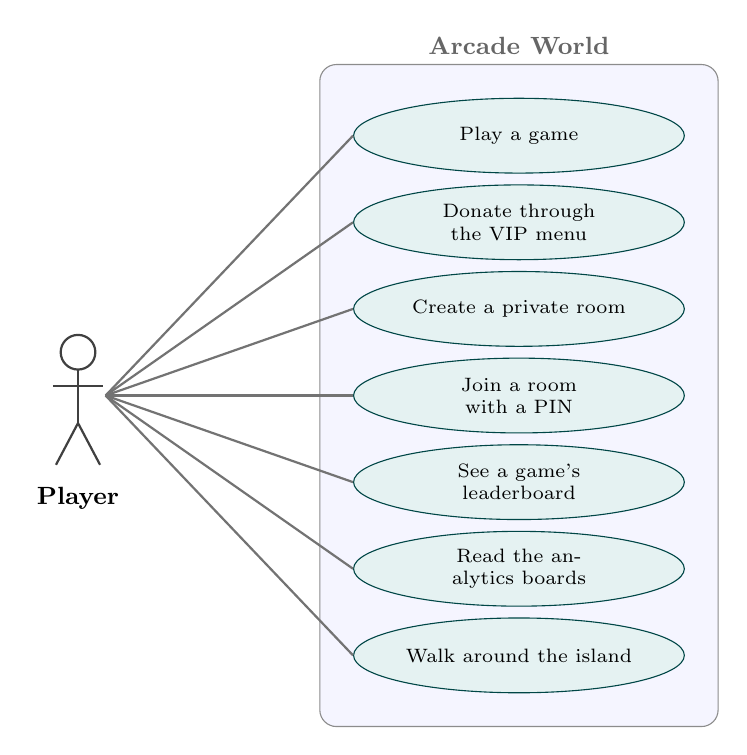
\begin{tikzpicture}[
  font=\small,
  ucase/.style={ellipse, draw=teal!55!black, fill=teal!10, align=center,
                font=\scriptsize, minimum height=0.95cm, text width=2.9cm, inner sep=1pt},
  assoc/.style={draw=black!55, thick},
]

% --- actor (stick figure) ---
\begin{scope}[shift={(0,0)}, thick, draw=black!75]
  \draw (0,0.55) circle (0.22);
  \draw (0,0.33) -- (0,-0.35);
  \draw (-0.32,0.12) -- (0.32,0.12);
  \draw (0,-0.35) -- (-0.28,-0.88);
  \draw (0,-0.35) -- (0.28,-0.88);
\end{scope}
\node[font=\small\bfseries] (player) at (0,-1.3) {Player};

% --- use cases ---
\node[ucase] (u1) at (5.6, 3.3)  {Play a game};
\node[ucase] (u2) at (5.6, 2.2)  {Donate through the VIP menu};
\node[ucase] (u3) at (5.6, 1.1)  {Create a private room};
\node[ucase] (u4) at (5.6, 0.0)  {Join a room with a PIN};
\node[ucase] (u5) at (5.6,-1.1)  {See a game's leaderboard};
\node[ucase] (u6) at (5.6,-2.2)  {Read the analytics boards};
\node[ucase] (u7) at (5.6,-3.3)  {Walk around the island};

% --- system boundary ---
\begin{scope}[on background layer]
  \node[draw=black!45, rounded corners=6pt, fill=blue!4, inner sep=12pt,
        fit=(u1)(u2)(u3)(u4)(u5)(u6)(u7),
        label={[font=\small\bfseries, black!60]north:Arcade World}] (box) {};
\end{scope}

% --- associations ---
\foreach \u in {u1,u2,u3,u4,u5,u6,u7} {
  \draw[assoc] (0.35,0) -- (\u.west);
}

\end{tikzpicture}

  \caption{Use case diagram of the player's actions inside the arcade world.}
  \label{fig:usecase}
\end{figure}

\subsection{Scenarios and Environments}

The game takes place in a single connected world, not in separate level screens. Inside this world, the player finds the ten arcade machines, each one a physical object they can walk up to and activate. The world also holds the global leaderboard boards and a bank themed building that shows live data about how every game is being played (this is explained later in the data analytics section). Everyone shares the same world, so one person can play a game while others watch or play on nearby machines.

\subsection{Death and Restart System}

Because the project is a collection of ten different games, there is no single rule for losing. Each game decides on its own when the run ends, but they all bring the player back to the same kind of game over screen afterwards, so the experience feels consistent across the whole arcade.

\subsubsection{Ways to Die}

\begin{table}[H]
\centering
\footnotesize
\begin{tabular}{|p{3.2cm}|p{12cm}|}
\hline
\textbf{Game} & \textbf{How the run ends} \\
\hline
Oxybelis & Crashing into a wall or into its own body. \\
\hline
Avis Toucan & Hitting a pipe or the ground. \\
\hline
Resilio & Losing all 3 lives when the ball falls below the paddle. \\
\hline
Foxy Fruit & Being caught by a bear; the run ends after all 3 lives are lost. \\
\hline
Firmament Defender & Losing all 4 lives to enemy fire, or any plane reaching the ship's row. \\
\hline
Firmament Siege & Losing all 3 lives to drone collisions. \\
\hline
Juice Cutter & Losing all lives by cutting the wrong fruits. \\
\hline
Turris Casei & A block missing the platform entirely. \\
\hline
Tap And Hold & Falling off a platform. \\
\hline
ImNotASphere & Losing all 8 lives by falling into a kill zone or off the level. \\
\hline
\end{tabular}
\caption{What ends the run in each game.}
\end{table}

\subsubsection{Restart System}

When a run ends, the player sees a game over screen with their final score and two options: play again or go back to the arcade. Playing again restarts that same game right away, so there is no loading and no need to walk back to the machine. Games that use lives (such as Resilio, Foxy Fruit, the Firmament games, and ImNotASphere) let the player respawn and keep going until all the lives are gone, and only then show the game over screen.

In the three multiplayer games (Turris Casei, Tap And Hold, ImNotASphere), a versus match does not end the moment one player dies. Instead, players who have been eliminated switch to spectator mode and can watch the others until the match finishes and a winner is chosen.

\subsection{Multiplatform}

All ten games run on PC, mobile, Xbox, and PlayStation from the same code. This works because every game sends its input through one shared controller layer. On PC it reads the keyboard and mouse, on console it reads the gamepad, and on mobile it shows touch controls on the screen that are built for that specific game (a direction pad, a single button, a joystick, and so on). The menus follow the same logic, so moving the selection and confirming a choice work the same way with a keyboard, a gamepad, or a tap on the screen. The player never has to pick a "mobile version" or a "console version"; the game simply adapts to whatever device is being used.

\section{Level Design}

\subsection{Description}

The ten games do not all handle levels in the same way. Some have a fixed number of handmade levels, some run forever and get harder over time, and some have no levels at all and simply keep going until the player loses. This variety is on purpose, because it keeps each machine feeling different from the one next to it.

\begin{table}[H]
\centering
\footnotesize
\begin{tabular}{|p{3.2cm}|p{3.2cm}|p{8.5cm}|}
\hline
\textbf{Game} & \textbf{Level Type} & \textbf{Description} \\
\hline
Oxybelis & Endless & One single grid; the game keeps going until the player crashes. The only goal is the score. \\
\hline
Avis Toucan & Infinite & Endless pipes that never stop; the run lasts as long as the player survives. \\
\hline
Resilio & Limited (5) & Five handmade brick layouts; clearing the last one is a perfect game. \\
\hline
Foxy Fruit & Limited (3) & Three handmade maze maps that get more complex as the player advances. \\
\hline
Firmament Defender & Limited (3) & Three waves that get faster each time. \\
\hline
Firmament Siege & Infinite & Endless survival; drones keep appearing and the game has no win state. \\
\hline
Juice Cutter & Limited (5) & Five levels, each one with its own fruit recipe and difficulty. \\
\hline
Turris Casei & Endless & Stack blocks until one misses the platform. \\
\hline
Tap And Hold & Infinite & Platforms generated on the fly that never end. \\
\hline
ImNotASphere & Limited (3) & Three handmade 3D levels with platforms, coins, and a finish line. \\
\hline
\end{tabular}
\caption{Level structure of each game.}
\end{table}

\subsection{Maps and Schemes}

\textit{To be updated.} The detailed maps and layout schemes for each game will be added in a future revision of this document.

\part{Engineering, Production and Launch}

\section{Technical Design}

\subsection{Game Engine}

The game was built entirely in \textbf{Roblox Studio}, using the Luau language. Server logic lives in ServerScriptService, shared game logic and physics live in ReplicatedStorage modules, and all interface, controls, and rendering live in StarterPlayer client scripts. The project is synced between Visual Studio Code and Roblox Studio using Rojo, which keeps the source code organized in a normal folder structure outside the engine.

\subsection{Development Schedule}

The project was built almost entirely alone and with no real prior experience in Roblox, so the pace was about one game per week. The focused work began on the first of February 2026, and the ten games were built one after another, each in roughly a week (around three days for the logic and three days to fix bugs and make it playable). After the ten games came one week of refactoring the code, one week writing this documentation, three weeks to design the island and its art, a longer stretch of testing and bug fixing across PC, mobile, and console, and finally one week to plan the marketing and record a trailer. With this pace, the planned release is the second week of July 2026. The Gantt chart below shows the order and the rough length of each part.

\begin{figure}[H]
  \centering
  \resizebox{\textwidth}{!}{\begin{ganttchart}[
  hgrid, vgrid,
  x unit=0.5cm,
  y unit title=0.62cm,
  y unit chart=0.52cm,
  title height=1,
  title/.style={fill=black!8, draw=black!30},
  title label font=\scriptsize\bfseries,
  bar height=0.6,
  bar/.style={fill=teal!45, draw=teal!60!black},
  bar label font=\scriptsize,
  group/.style={fill=blue!45, draw=blue!60!black},
  group label font=\scriptsize\bfseries,
  group height=0.5,
  milestone/.style={fill=orange!70, draw=orange!80!black},
  milestone label font=\scriptsize\bfseries,
]{1}{23}

\gantttitle{Feb 2026}{4}
\gantttitle{Mar 2026}{4}
\gantttitle{Apr 2026}{5}
\gantttitle{May 2026}{4}
\gantttitle{Jun 2026}{4}
\gantttitle{Jul}{2} \\

\ganttgroup{2D classic games}{1}{7} \\
\ganttbar{Oxybelis}{1}{1} \\
\ganttbar{Avis Toucan}{2}{2} \\
\ganttbar{Resilio}{3}{3} \\
\ganttbar{Foxy Fruit}{4}{4} \\
\ganttbar{Firmament Defender}{5}{5} \\
\ganttbar{Firmament Siege}{6}{6} \\
\ganttbar{Juice Cutter}{7}{7} \\

\ganttgroup{3D multiplayer games}{8}{10} \\
\ganttbar{Turris Casei}{8}{8} \\
\ganttbar{Tap And Hold}{9}{9} \\
\ganttbar{ImNotASphere}{10}{10} \\

\ganttgroup{Polish, art and release}{11}{23} \\
\ganttbar{Code refactoring}{11}{11} \\
\ganttbar{Documentation}{12}{12} \\
\ganttbar{Island and art design}{13}{15} \\
\ganttbar{Testing and bug fixing}{16}{21} \\
\ganttbar{Marketing and trailer}{22}{22} \\
\ganttmilestone{Release}{23}

\end{ganttchart}
}
  \caption{Development schedule, from the first game in February 2026 to the planned release in the second week of July 2026.}
  \label{fig:gantt_schedule}
\end{figure}

The next chart breaks down the work for each game into the two phases: the days spent on the logic and the days spent polishing and fixing bugs. It makes clear that the 3D multiplayer games (Turris Casei, Tap And Hold, and ImNotASphere) were the most expensive, while the first and simplest games were the quickest.

\begin{figure}[H]
  \centering
  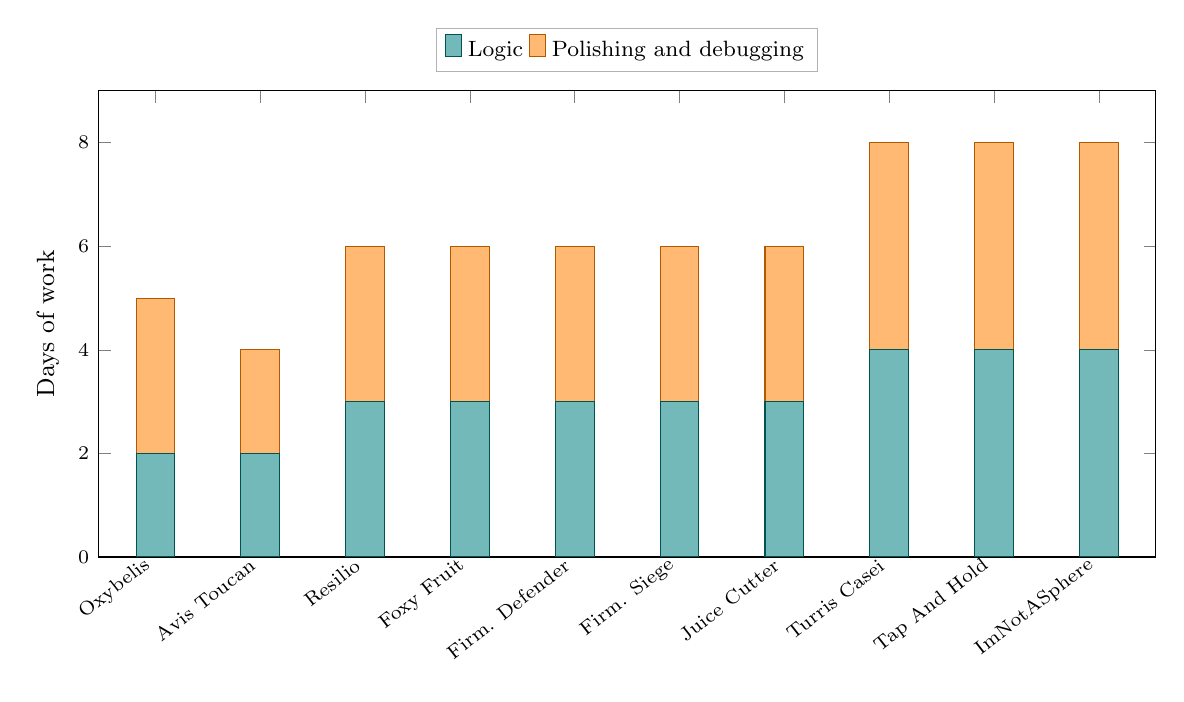
\begin{tikzpicture}
\begin{axis}[
  ybar stacked,
  bar width=14pt,
  width=15cm, height=7.5cm,
  symbolic x coords={Oxybelis,Avis Toucan,Resilio,Foxy Fruit,Firm. Defender,Firm. Siege,Juice Cutter,Turris Casei,Tap And Hold,ImNotASphere},
  xtick=data,
  x tick label style={rotate=38, anchor=east, font=\scriptsize},
  ylabel={Days of work},
  ymin=0, ymax=9,
  ytick={0,2,4,6,8},
  enlarge x limits=0.06,
  legend style={at={(0.5,1.04)}, anchor=south, legend columns=-1, font=\footnotesize, draw=black!30},
  tick label style={font=\scriptsize},
  ylabel style={font=\small},
  nodes near coords align={vertical},
]
\addplot+[ybar, fill=teal!55, draw=teal!65!black] coordinates {
  (Oxybelis,2) (Avis Toucan,2) (Resilio,3) (Foxy Fruit,3) (Firm. Defender,3)
  (Firm. Siege,3) (Juice Cutter,3) (Turris Casei,4) (Tap And Hold,4) (ImNotASphere,4) };
\addplot+[ybar, fill=orange!55, draw=orange!70!black] coordinates {
  (Oxybelis,3) (Avis Toucan,2) (Resilio,3) (Foxy Fruit,3) (Firm. Defender,3)
  (Firm. Siege,3) (Juice Cutter,3) (Turris Casei,4) (Tap And Hold,4) (ImNotASphere,4) };
\legend{Logic, Polishing and debugging}
\end{axis}
\end{tikzpicture}

  \caption{Days of work per game, split into logic and polishing or debugging.}
  \label{fig:barchart_days}
\end{figure}

\subsection{Optimization}

Because the arcade has to run smoothly on phones and consoles, every game was written with its performance cost in mind. Most game loops were kept at a constant or almost constant cost per frame, and memory use was always kept within a fixed limit, so nothing grows out of control during a session. The table below gives a short summary for each game; the detailed analysis is in each game's own section earlier in this document.

\begin{table}[H]
\centering
\footnotesize
\begin{tabular}{|p{3.2cm}|p{7cm}|p{5cm}|}
\hline
\textbf{Game} & \textbf{Cost per tick} & \textbf{Memory} \\
\hline
Oxybelis & $O(1)$ via a circular buffer & $O(N)$, fixed grid (192 cells) \\
\hline
Avis Toucan & $O(P)$ with $P \leq 3$ pipes, so $O(1)$ & $O(P)$, bounded \\
\hline
Resilio & $O(B)$ bricks, decreasing per level & $O(B)$, $B \leq 120$ \\
\hline
Foxy Fruit & $O(E \times N)$ with $E=4$, $N=192$ fixed & $O(N)$, fixed grid \\
\hline
Firmament Defender & $O(N)$ planes, $N \leq 30$, decreasing & $O(N)$, bounded \\
\hline
Firmament Siege & $O(N \times M)$ with $N \leq 7$, $M \leq 10$ & $O(N+M)$, bounded \\
\hline
Juice Cutter & $O(F)$ fruits, $F \leq 10$, so $O(1)$ & $O(F)$, bounded \\
\hline
Turris Casei & $O(1)$ per block drop & $O(1)$ game logic \\
\hline
Tap And Hold & $O(1)$ per jump & $O(1)$, max 4 platforms \\
\hline
ImNotASphere & $O(1)$ per physics tick (stateless module) & $O(1)$ game logic \\
\hline
\end{tabular}
\caption{Optimization summary for each game. The three multiplayer games also keep $O(P)$ lobby data for up to $P \leq 50$ players (10 for ImNotASphere).}
\end{table}

\subsection{System Requirements}

Because the game runs on the Roblox platform, the requirements match Roblox's own minimum requirements rather than custom hardware targets.

\subsubsection{PC}

\begin{itemize}
  \item Windows 10 or newer (or macOS 10.13+).
  \item A processor from 2015 or later, with at least 4 cores (around 2.5\,GHz or faster).
  \item At least 8\,GB of RAM.
  \item An internet connection (the game is online and uses DataStore for leaderboards).
  \item Keyboard and mouse.
\end{itemize}

\subsubsection{Mobile (Android and iOS)}

\begin{itemize}
  \item Android: any device running Android 10 or newer with at least 8\,GB of RAM.
  \item iOS: iPhone 14 or newer.
  \item A touchscreen (the touch controls are built automatically).
  \item An internet connection.
\end{itemize}

\subsubsection{Xbox Series S/X}

\begin{itemize}
  \item An Xbox console that supports the Roblox app (Xbox One and Series S/X).
  \item An Xbox controller (the gamepad layout is supported in every game).
  \item An internet connection.
\end{itemize}

\subsubsection{PlayStation}

\begin{itemize}
  \item A PlayStation console that supports the Roblox app (PS4 and PS5).
  \item A DualSense or DualShock controller (same gamepad layout as Xbox).
  \item An internet connection.
\end{itemize}

\subsection{Testing and QA}

The testing was done by hand, one piece at a time, since the project was built alone. There was no automated test suite; instead, each part was checked directly inside Roblox Studio while it was being built, and again after each change. The focus was always the same: make sure the game stays playable and that nothing breaks the calm feeling of the world.

The main things that were checked, game by game, were:

\begin{itemize}
  \item \textbf{Menus:} that every screen opens and closes correctly, that the PLAY, VIP, EXIT, and MENU buttons go where they should, and that the donation menu shows the right products.
  \item \textbf{Sounds:} that each sound plays at the right moment (scoring, losing, selecting), and that the mute button turns all audio on and off.
  \item \textbf{Buttons and input:} that every button reacts to a click and a tap, and that the keyboard controls (WASD, arrow keys, Space) work in each game.
  \item \textbf{Mobile:} using the device emulator inside Roblox Studio to act like a phone, checking that the on screen touch controls appear, that they are placed well, and that the games can be fully played with touch.
  \item \textbf{Gamepad:} that the menus and the games respond to a controller, so the Xbox and PlayStation layouts behave like the keyboard one.
  \item \textbf{Leaderboards and saving:} that a finished game reports its score, that the top 10 boards update, and that audio settings come back correctly after rejoining.
\end{itemize}

Each game was only marked as working once it had passed these checks on PC and in the mobile emulator. The known gaps and anything still pending are listed in the per game feature tables earlier in this document.

\section{Marketing Plan}

This game is a portfolio and learning project, not a commercial product, so the marketing plan has two simple goals: cover the running costs of the game, and reach the kind of player who would really enjoy it. The audience is very specific. These are solo and casual players who are not competitive and do not need to play with friends. For that reason, the plan skips the usual tactics aimed at hardcore or social audiences and focuses on simple discovery instead: a person sees the game in under a minute, learns its name, and decides to give it a try.

\subsection{Monetization}

All the money side of the game is optional and never makes the game easier to play. Nothing can be bought to gain an advantage, and all the income is meant to cover the running costs and help fund a future project. There are four ways the game can earn money, three of them already working and one still being studied:

\begin{itemize}
  \item \textbf{Developer product donations (VIP menu).} Every game has a VIP menu with several donation tiers (from 5 up to 1000 Robux). These are pure donations: the player gets nothing that changes the gameplay, they simply support the project if they want to. This is already working in all ten games.
  \item \textbf{VIP rooms (single purchase).} A VIP area inside the map, sold as a single purchase instead of a monthly subscription. Once a player buys it, they keep access forever. This gives supporters a special space without splitting the players apart or locking any game behind a paywall.
  \item \textbf{Private server rental.} Players can rent a private server through the system that Roblox already provides. This fits the private style of the game's multiplayer (rooms protected by a PIN), giving small groups their own space to play together.
  \item \textbf{Immersive advertising (being studied).} Roblox has an immersive ad system that places ad surfaces inside the 3D world. It is being considered as an extra source of income, but it is not active yet, because it first has to be tested to make sure it does not hurt the calm and relaxed feeling of the world.
\end{itemize}

\subsection{Marketing Strategy}

The marketing only starts once the game is \textbf{100\% finished}. Promoting an unfinished game to a casual audience usually backfires: a new player who runs into a bug or a missing image simply leaves and does not come back. So the plan is to wait until the experience is complete and polished, and only then push hard with short videos.

The whole strategy rests on one idea: \textbf{a person should understand the game, see its name, and want to try it, all in under one minute.} Casual and solo players do not find games through tournaments, ads, or friends telling them about it. They find them by scrolling through short videos and thinking ``that looks fun, let me try it.'' The campaign is built entirely around that moment.

\subsubsection{Channels}

\begin{itemize}
  \item \textbf{Short videos} (TikTok, YouTube Shorts, Instagram Reels): the main channel. Vertical clips under 60 seconds, each one showing a single game in action with the game name on the screen the whole time.
  \item \textbf{YouTube (longer videos):} a second channel for longer content, such as full gameplay and videos aimed at other developers. Every YouTube description links to the \textbf{GitHub repository}, so anyone who wants the full source code and documentation can find it. This reaches a second, smaller audience: people who are learning to make games in Roblox.
\end{itemize}

\subsubsection{Content Plan}

\begin{itemize}
  \item \textbf{One video per game.} At least ten short clips, one for each game, so every machine gets its own moment. The first three seconds show the most striking part, and the name of the game stays on the screen the whole time so viewers can search for it.
  \item \textbf{Hook first, name always.} Every clip opens with the most fun or surprising moment, never a slow intro. The name of the game and the name of the world are always visible, because the goal is for people to remember it, not just to watch it.
  \item \textbf{Lean into the relaxed, playful tone.} The audience includes people who enjoy weird, charming, low pressure games. The clips should feel calm and a little playful, matching the tone of the world instead of hyping up competition.
  \item \textbf{Compilations.} Short montages that show several games one after another make the main selling point clear: ten games in one place, eight minutes of variety.
  \item \textbf{Familiar arcade styles.} Many of the games are classic arcade styles rebuilt inside a 3D world. The clips can use that familiarity, since players often already know how to play, which makes them more willing to try it.
\end{itemize}

\subsubsection{Rollout Phases}

\begin{enumerate}
  \item \textbf{Before launch (teasers).} A few short clips with quick glimpses of the world and some of the games, to build a little curiosity before release.
  \item \textbf{Launch.} When the game is fully finished, release the ten clips (one per game) close together across TikTok, Shorts, and Reels, plus one or two compilations.
  \item \textbf{After launch.} Keep posting regularly, paying attention to which clips do best and to whatever is trending in short video, and always keeping the name of the game and the world at the center.
\end{enumerate}

\subsection{Why This Fits the Audience}

The game is made for people who want to try a new game, enjoy a meme game, relax with something low stress, or replay classic arcade styles inside Roblox. These players are reached through discovery, not persuasion. Short videos are a perfect match: they deliver the ``that looks fun'' moment in seconds, they do not ask the viewer to commit to anything, and they spread on their own when a clip is charming enough. The GitHub link on YouTube adds a second layer, turning the project into both a game that people play and a learning resource that other developers can study.

\part{Technical Implementation}

\section{System Architecture Overview}

Before going into the details of each part, the diagram below gives a single bird's eye view of the whole project. It shows how everything connects: the player interacts with the game world, the client reads the input and draws the screen, the client and the server talk through RemoteEvents and RemoteFunctions, the server uses the shared modules for the game logic, and the modules read and write to the Roblox DataStore. The same five layers are reused by all ten games and by the shared systems.

\begin{figure}[H]
  \centering
  \resizebox{\textwidth}{!}{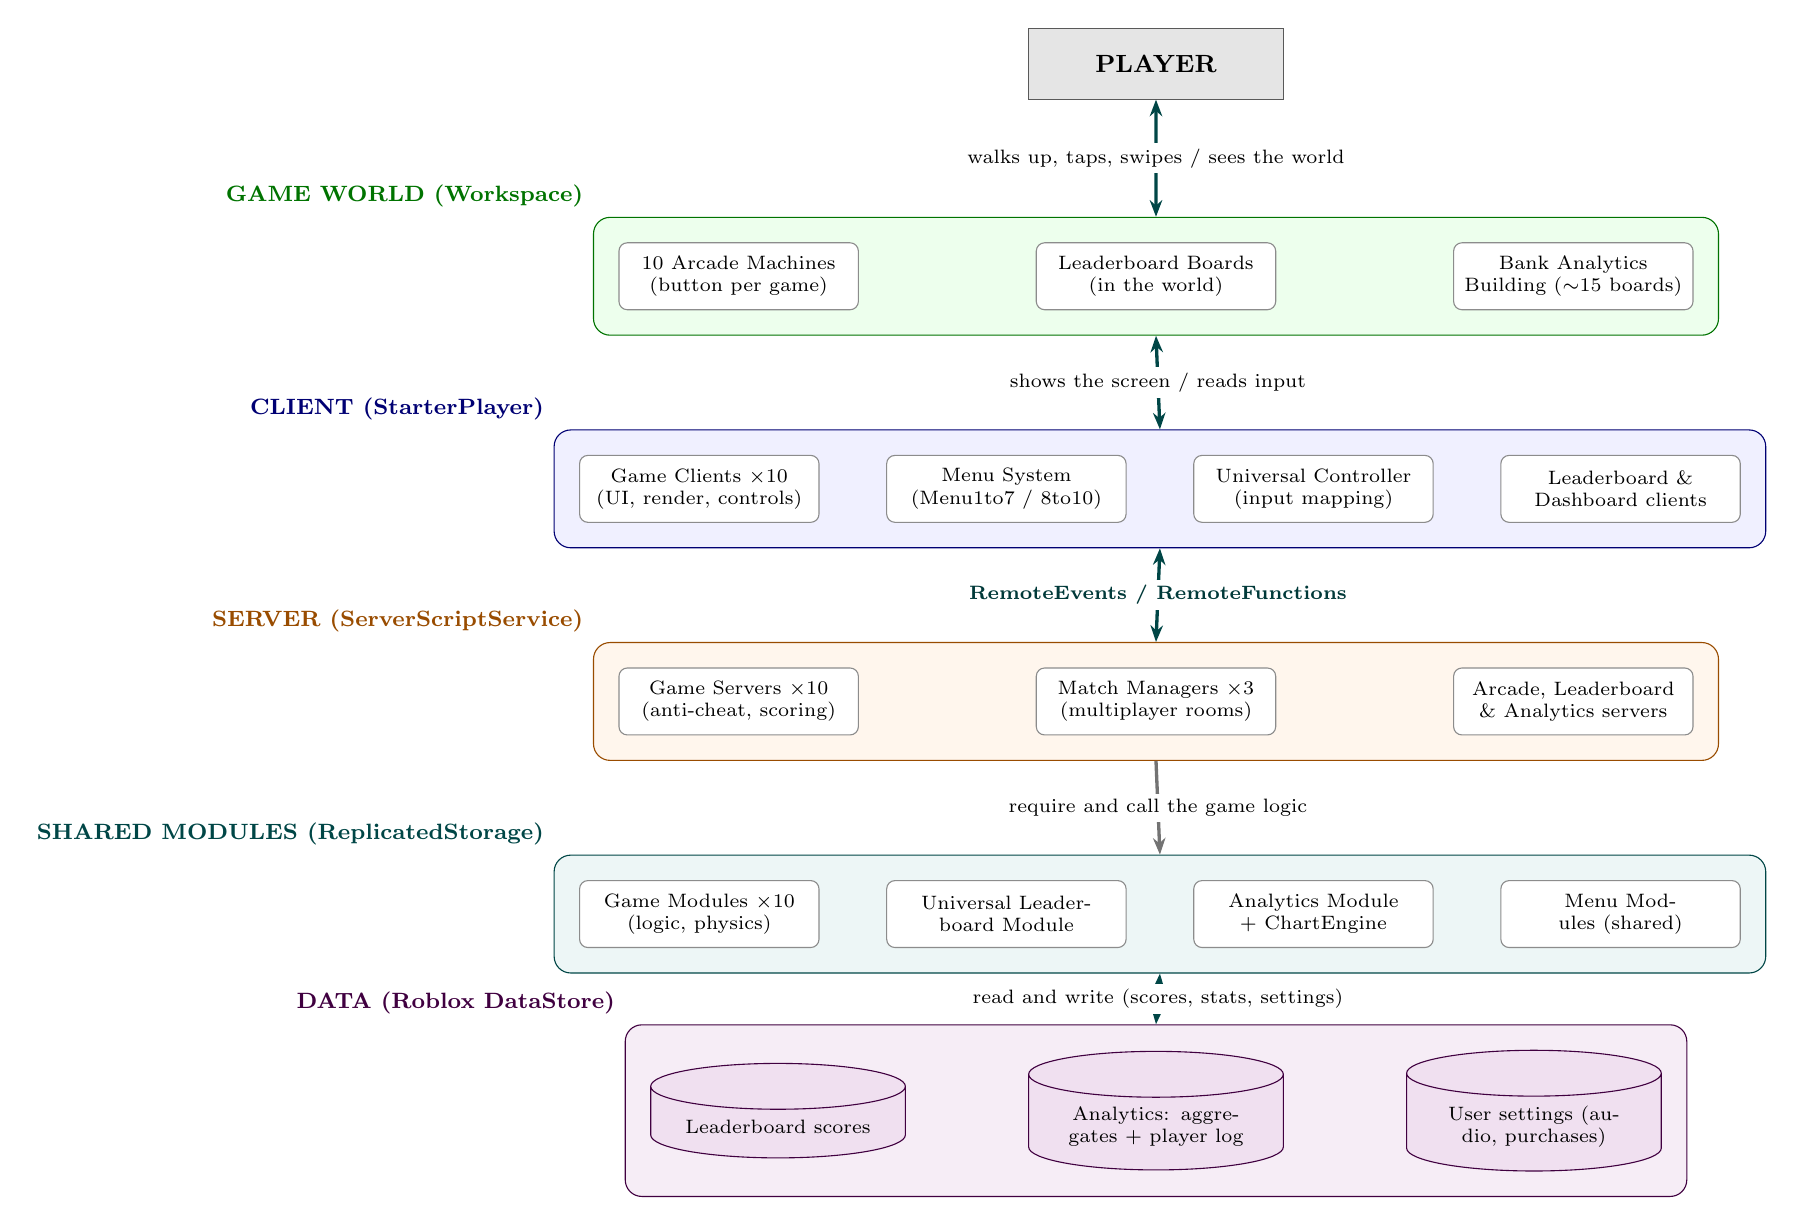
\begin{tikzpicture}[
  font=\small,
  >={Stealth[length=6pt]},
  item/.style={rectangle, rounded corners=3pt, draw=black!45, fill=white,
               align=center, font=\scriptsize, minimum height=0.85cm, text width=2.9cm, inner sep=2pt},
  store/.style={cylinder, shape border rotate=90, aspect=0.18, draw=violet!50!black,
                fill=violet!12, align=center, font=\scriptsize, text width=3.0cm, minimum height=1.2cm},
  entity/.style={rectangle, draw=black!65, fill=black!10, align=center,
                 font=\small\bfseries, minimum height=0.9cm, text width=3cm},
  lbl/.style={font=\footnotesize\bfseries},
  flow/.style={->, very thick, draw=black!55},
  net/.style={<->, very thick, draw=teal!55!black},
]

% --- nodes per layer ---
\node[entity] (player) at (8,0.7) {PLAYER};

\node[item] (w1) at (2.7,-2.0)  {10 Arcade Machines (button per game)};
\node[item] (w2) at (8.0,-2.0)  {Leaderboard Boards (in the world)};
\node[item] (w3) at (13.3,-2.0) {Bank Analytics Building ($\sim$15 boards)};

\node[item] (c1) at (2.2,-4.7)  {Game Clients $\times 10$ (UI, render, controls)};
\node[item] (c2) at (6.1,-4.7)  {Menu System (Menu1to7 / 8to10)};
\node[item] (c3) at (10.0,-4.7) {Universal Controller (input mapping)};
\node[item] (c4) at (13.9,-4.7) {Leaderboard \& Dashboard clients};

\node[item] (s1) at (2.7,-7.4)  {Game Servers $\times 10$ (anti-cheat, scoring)};
\node[item] (s2) at (8.0,-7.4)  {Match Managers $\times 3$ (multiplayer rooms)};
\node[item] (s3) at (13.3,-7.4) {Arcade, Leaderboard \& Analytics servers};

\node[item] (m1) at (2.2,-10.1) {Game Modules $\times 10$ (logic, physics)};
\node[item] (m2) at (6.1,-10.1) {Universal Leaderboard Module};
\node[item] (m3) at (10.0,-10.1){Analytics Module + ChartEngine};
\node[item] (m4) at (13.9,-10.1){Menu Modules (shared)};

\node[store] (d1) at (3.2,-12.8) {Leaderboard scores};
\node[store] (d2) at (8.0,-12.8) {Analytics: aggregates + player log};
\node[store] (d3) at (12.8,-12.8){User settings (audio, purchases)};

% --- layer containers (drawn behind) ---
\begin{scope}[on background layer]
  \node[rounded corners=6pt, fill=green!7,  draw=green!45!black, inner sep=9pt,
        fit=(w1)(w2)(w3), label={[lbl, green!45!black]north west:GAME WORLD (Workspace)}] (worldbox) {};
  \node[rounded corners=6pt, fill=blue!6,   draw=blue!45!black, inner sep=9pt,
        fit=(c1)(c2)(c3)(c4), label={[lbl, blue!45!black]north west:CLIENT (StarterPlayer)}] (clientbox) {};
  \node[rounded corners=6pt, fill=orange!7, draw=orange!60!black, inner sep=9pt,
        fit=(s1)(s2)(s3), label={[lbl, orange!60!black]north west:SERVER (ServerScriptService)}] (serverbox) {};
  \node[rounded corners=6pt, fill=teal!7,   draw=teal!55!black, inner sep=9pt,
        fit=(m1)(m2)(m3)(m4), label={[lbl, teal!55!black]north west:SHARED MODULES (ReplicatedStorage)}] (modbox) {};
  \node[rounded corners=6pt, fill=violet!7, draw=violet!50!black, inner sep=9pt,
        fit=(d1)(d2)(d3), label={[lbl, violet!50!black]north west:DATA (Roblox DataStore)}] (databox) {};
\end{scope}

% --- flows between layers ---
\draw[net] (player) -- node[font=\scriptsize, fill=white, inner sep=2pt]{walks up, taps, swipes / sees the world} (worldbox.north);
\draw[net] (worldbox.south) -- node[font=\scriptsize, fill=white, inner sep=2pt]{shows the screen / reads input} (clientbox.north);
\draw[net] (clientbox.south) -- node[font=\scriptsize, fill=white, inner sep=2pt, text=teal!45!black]{\textbf{RemoteEvents / RemoteFunctions}} (serverbox.north);
\draw[flow] (serverbox.south) -- node[font=\scriptsize, fill=white, inner sep=2pt]{require and call the game logic} (modbox.north);
\draw[net] (modbox.south) -- node[font=\scriptsize, fill=white, inner sep=2pt]{read and write (scores, stats, settings)} (databox.north);

\end{tikzpicture}
}
  \caption{Bird's eye view of the system. Five layers, from the player at the top down to the DataStore, shared by the ten games, the leaderboards, the menus, the controller, and the analytics.}
  \label{fig:architecture_overview}
\end{figure}

\clearpage

\section{Roblox Structure}

\begin{lstlisting}[caption={Current project structure in Roblox (Updated with Avis Toucan, Oxybelis, Resilio, Foxy Fruit, Firmament Defender, Firmament Siege, Juice Cutter, Universal Leaderboard, and the Data Analytics System).},label={lst:roblox-structure-final}]
.
|-- Workspace
|   +-- UniversalLeaderboardPart (Part, Tag="LeadboradAvisToucan", Attribute="GAMEID=AvisToucan")
|   +-- UniversalLeaderboardPart (Part, Tag="LeadboradOxybelis", Attribute="GAMEID=Oxybelis")
|   +-- UniversalLeaderboardPart (Part, Tag="LeadboradResilio", Attribute="GAMEID=Resilio")
|   +-- UniversalLeaderboardPart (Part, Tag="LeadboradFoxyFruit", Attribute="GAMEID=FoxyFruit")
|   +-- UniversalLeaderboardPart (Part, Tag="LeadboradFirmamentDefender", Attribute="GAMEID=FirmamentDefender")
|   +-- UniversalLeaderboardPart (Part, Tag="LeadboradFirmamentSiege", Attribute="GAMEID=FirmamentSiege")
|   +-- UniversalLeaderboardPart (Part, Tag="LeadboradJuiceCutter", Attribute="GAMEID=JuiceCutter")
|   +-- TurrisCaseiLeaderboardPart (Score Table)
|   +-- TapAndHoldLeaderboardPart (Score Table)
|   +-- ImNotASphereLeaderboardPart (Score Table)
|   +-- Oxybelis (Folder)
|   |   +-- ButtonOxybelis (Part, Tag="ButtonOxybelis")
|   +-- AvisToucan (Folder)
|   |   +-- ButtonAvisToucan (Part, Tag="ButtonAvisToucan")
|   +-- Resilio (Folder)
|   |   +-- ButtonResilio (Part, Tag="ButtonResilio")
|   +-- FoxyFruit (Folder)
|   |   +-- ButtonFoxyFruit (Part, Tag="ButtonFoxyFruit")
|   +-- FirmamentDefender (Folder)
|   |   +-- ButtonFirmamentDefender (Part, Tag="ButtonFirmamentDefender")
|   +-- FirmamentSiege (Folder)
|   |   +-- ButtonFirmamentSiege (Part, Tag="ButtonFirmamentSiege")
|   +-- JuiceCutter (Folder)
|   |   +-- ButtonJuiceCutter (Part, Tag="ButtonJuiceCutter")
|   +-- TurrisCasei (Folder)
|   |   +-- ButtonTurrisCasei (Part, Tag="TurrisTerminal")
|   +-- TapAndHold (Folder)
|   |   +-- ButtonTapAndHold (Part, Tag="TapAndHoldTerminal")
|   +-- ImNotASphere (Folder)
|   |   +-- ButtonImNotASphere (Part, Tag="ImNotASphereTerminal")
|   +-- BankBuilding (Model, themed data analytics area)
|       +-- AnalyticsBoard x10 (Part, Tag="AnalyticsBoard", Attribute="GameId=<game>")
|       +-- AnalyticsBoard (Part, Tag="AnalyticsBoard", Attribute="GameId=General")
|       +-- AnalyticsBoard (Part, Tag="AnalyticsBoard", Attribute="GameId=Money")
|       +-- AnalyticsBoard (Part, Tag="AnalyticsBoard", Attribute="GameId=MoneyG")
|       +-- AnalyticsBoard (Part, Tag="AnalyticsBoard", Attribute="GameId=RealMoney")
|       +-- AnalyticsBoard (Part, Tag="AnalyticsBoard", Attribute="GameId=RealPlayer")
|       +-- AnalyticsBoard (Part, Tag="AnalyticsBoard", Attribute="GameId=LastMessage")
|-- ReplicatedStorage
|   +-- ArcadeRemotes
|   |   +-- OpenArcadeMenu (RemoteEvent)
|   |   +-- GlobalBoard (Folder)
|   |   |   +-- UpdateUniversalLeaderboard (RemoteEvent)
|   |   +-- AvisToucan (Folder)
|   |   |   +-- StartAvisToucanRequest (RemoteEvent)
|   |   |   +-- SubmitFlap (RemoteEvent)
|   |   |   +-- GameState (RemoteEvent)
|   |   |   +-- ToggleAudio (RemoteEvent)
|   |   +-- Oxybelis (Folder)
|   |   |   +-- StartOxybelisRequest (RemoteEvent)
|   |   |   +-- SubmitMove (RemoteEvent)
|   |   |   +-- GameState (RemoteEvent)
|   |   |   +-- ToggleAudio (RemoteEvent)
|   |   +-- Resilio
|   |   |   +-- StartResilioRequest (RemoteEvent)
|   |   |   +-- SubmitMoveInput (RemoteEvent)
|   |   |   +-- SubmitLaunch (RemoteEvent)
|   |   |   +-- GameState (RemoteEvent)
|   |   |   +-- ToggleAudio (RemoteEvent)
|   |   +-- FoxyFruit
|   |   |   +-- StartFoxyFruitRequest (RemoteEvent)
|   |   |   +-- SubmitMove (RemoteEvent)
|   |   |   +-- GameState (RemoteEvent)
|   |   |   +-- ToggleAudio (RemoteEvent)
|   |   +-- FirmamentDefender
|   |   |   +-- StartFirmamentDefenderRequest (RemoteEvent)
|   |   |   +-- SubmitMove (RemoteEvent)
|   |   |   +-- GameState (RemoteEvent)
|   |   |   +-- ToggleAudio (RemoteEvent)
|   |   +-- FirmamentSiege
|   |   |   +-- StartFirmamentSiegeRequest (RemoteEvent)
|   |   |   +-- SubmitMove (RemoteEvent)
|   |   |   +-- GameState (RemoteEvent)
|   |   |   +-- ToggleAudio (RemoteEvent)
|   |   +-- JuiceCutter
|   |   |   +-- StartJuiceCutterRequest (RemoteEvent)
|   |   |   +-- SubmitMove (RemoteEvent)
|   |   |   +-- GameState (RemoteEvent)
|   |   |   +-- ToggleAudio (RemoteEvent)
|   |   +-- TurrisCasei
|   |   |   +-- StartTurrisCaseiRequest (RemoteEvent)
|   |   |   +-- MatchStatus (RemoteEvent)
|   |   |   +-- ToggleAudio (RemoteEvent)
|   |   |   +-- UpdateTurrisCaseiLeaderboard (RemoteEvent)
|   |   |   +-- GetAudioState (RemoteFunction)
|   |   |   +-- LobbySystem (Folder)
|   |   |       +-- CreateRoom (RemoteFunction)
|   |   |       +-- JoinRoom (RemoteFunction)
|   |   |       +-- StartMultiplayerMatch (RemoteEvent)
|   |   |       +-- RoomUpdate (RemoteEvent)
|   |   |       +-- KickPlayer (RemoteEvent)
|   |   |       +-- LeaveRoom (RemoteEvent)
|   |   |       +-- UpdateLiveScore (RemoteEvent)
|   |   |       +-- SpectateTarget (RemoteEvent)
|   |   |       +-- PlayerDied (RemoteEvent)
|   |   +-- TapAndHold
|   |   |   +-- StartTapAndHoldRequest (RemoteEvent)
|   |   |   +-- SubmitJumpCharge (RemoteEvent)
|   |   |   +-- MatchStatus (RemoteEvent)
|   |   |   +-- ToggleAudio (RemoteEvent)
|   |   |   +-- UpdateTapAndHoldLeaderboard (RemoteEvent)
|   |   |   +-- GetAudioState (RemoteFunction)
|   |   |   +-- LobbySystem (Folder)
|   |   |       +-- CreateRoom (RemoteFunction)
|   |   |       +-- JoinRoom (RemoteFunction)
|   |   |       +-- StartMultiplayerMatch (RemoteEvent)
|   |   |       +-- RoomUpdate (RemoteEvent)
|   |   |       +-- KickPlayer (RemoteEvent)
|   |   |       +-- LeaveRoom (RemoteEvent)
|   |   |       +-- UpdateLiveScore (RemoteEvent)
|   |   |       +-- SpectateTarget (RemoteEvent)
|   |   |       +-- PlayerDied (RemoteEvent)
|   |   +-- ImNotASphere
|   |       +-- StartImNotASphereRequest (RemoteEvent)
|   |       +-- MatchStatus (RemoteEvent)
|   |       +-- ToggleAudio (RemoteEvent)
|   |       +-- UpdateImNotASphereLeaderboard (RemoteEvent)
|   |       +-- GetAudioState (RemoteFunction)
|   |       +-- LobbySystem (Folder)
|   |           +-- CreateRoom (RemoteFunction)
|   |           +-- JoinRoom (RemoteFunction)
|   |           +-- StartMultiplayerMatch (RemoteEvent)
|   |           +-- RoomUpdate (RemoteEvent)
|   |           +-- KickPlayer (RemoteEvent)
|   |           +-- LeaveRoom (RemoteEvent)
|   |           +-- UpdateLiveScore (RemoteEvent)
|   |           +-- SpectateTarget (RemoteEvent)
|   |           +-- PlayerDied (RemoteEvent)
|   +-- AnalyticsRemotes (Folder)
|   |   +-- GetGameDashboard (RemoteFunction)
|   |   +-- GetGeneralDashboard (RemoteFunction)
|   |   +-- GetMoneyDashboard (RemoteFunction)
|   |   +-- GetRecentDonations (RemoteFunction)
|   |   +-- GetRecentScores (RemoteFunction)
|   |   +-- DashboardUpdated (RemoteEvent)
|   +-- Menu (Folder)
|   |   +-- Menu1to7 (ModuleScript)
|   |   +-- Menu8to10 (ModuleScript)
|   +-- TurrisCasei_Assets (Folder)
|   |   +-- BaseP1 (Part/Model)
|   |   +-- QuesoBlock (Part)
|   |   +-- RoomModel (Model)
|   +-- TapAndHold_Assets (Folder)
|   |   +-- tapsuelo1..tapsuelo4 (Platform)
|   |   +-- Model (Model floor)
|   +-- ImNotASphere_Assets (Folder)
|       +-- PlayerSphere (Part player)
|       +-- Level1 (Model)
|       |   +-- Geometry (Folder - Optional)
|       |   |   +-- Suelo1, Rampa2, Pared3 (Parts)
|       |   +-- MovingPlatforms (Folder)
|       |   |   +-- Elevator1 (Model)
|       |   |       +-- Platform (Moving part)
|       |   |       +-- StartPart (Transparent, CanCollide=false)
|       |   |       +-- EndPart (Transparent, CanCollide=false)
|       |   +-- Collectibles (Folder)
|       |   |   +-- Coin (Part)
|       |   |   +-- ExtraPoint (Part)
|       |   +-- KillZones (Folder)
|       |   |   +-- DeathPit (Giant transparent part below level)
|       |   +-- SpawnPoint (Transparent part)
|       |   +-- FinishLine (Part - Goal to proceed to Level2)
|       +-- Level2, Level3 (Models)
|   +-- Modules
|       +-- UniversalLeaderboardModule (ModuleScript: Global Score logic)
|       +-- TurrisCaseiLeaderboard (score turris casei)
|       +-- TapAndHoldLeaderboard (score Tap-and-Hold)
|       +-- ImNotASphereLeaderboard (ModuleScript: Score table logic)
|       +-- AvisToucanModule (ModuleScript logic,physics,collisions,etc)
|       +-- OxybelisModule (ModuleScript logic,physics,collisions,etc)
|       +-- ResilioModule (ModuleScript logic,physics,collisions,etc)
|       +-- FoxyFruitModule (ModuleScript logic,physics,collisions,etc)
|       +-- FirmamentDefenderModule (ModuleScript logic,physics,collisions,etc)
|       +-- FirmamentSiegeModule (ModuleScript logic,physics,collisions,etc)
|       +-- JuiceCutterModule (ModuleScript logic,physics,collisions,etc)
|       +-- TurrisCaseiModule (ModuleScript math,speed,physics)
|       +-- TapAndHoldModule (ModuleScript logic,physics,parabolic math)
|       +-- ImNotASphereModule (ModuleScript: Physics, speed, powers, elevator math)
|       +-- AnalyticsModule (ModuleScript: session/donation tracking, aggregates, dashboards)
|       +-- ChartEngine (ModuleScript: draws charts on EditableImage canvases)
|-- ServerScriptService
|   +-- UniversalLeaderboardServer.lua (Script: Global Data Broadcast)
|   +-- ArcadeServer.lua (Script:binds buttons by tag,sends OpenArcadeMenu)
|   +-- AvisToucanServer.lua (Script:button and input connections)
|   +-- OxybelisServer.lua (Script:button and input connections)
|   +-- ResilioServer.lua (Script:button and input connections)
|   +-- FoxyFruitServer.lua (Script:button and input connections)
|   +-- FirmamentDefenderServer.lua (Script:button and input connections)
|   +-- FirmamentSiegeServer.lua (Script:button and input connections)
|   +-- JuiceCutterServer.lua (Script:button and input connections)
|   +-- TurrisCaseiServer.lua (Script: Anti-Cheat & Global Data)
|   +-- TurrisCaseiMatchManager.lua (ModuleScript: versus logic, rooms, winner selection)
|   +-- TapAndHoldServer.lua (Script: Anti-Cheat & Global Data)
|   +-- TapAndHoldMatchManager.lua (ModuleScript: versus logic, rooms, winner selection)
|   +-- ImNotASphereServer.lua (Script: Anti-Cheat, Power up validation & Global Data)
|   +-- ImNotASphereMatchManager.lua (ModuleScript: versus logic, rooms, winner selection)
|   +-- AnalyticsServer.lua (Script: analytics remotes, rate limiting, refresh broadcast)
|   +-- SunsetAtmosphere.lua (Script: world lighting and ambiance)
|   +-- GodRays.lua (Script: sun ray visual effect)
|-- StarterPlayer
|   +-- StarterPlayerScripts
|       +-- UniversalController.lua (ModuleScript: Mapping for mobile, pc, xbox, playstation)
|       +-- UniversalLeaderboardClient.lua (LocalScript: Multi-game dynamic UI renderer)
|       +-- AvisToucanClient.lua (LocalScript: arcade UI/menu, render, controls)
|       +-- OxybelisClient.lua (LocalScript: arcade UI/menu, render, controls)
|       +-- ResilioClient.lua (LocalScript: arcade UI/menu, render, controls)
|       +-- FoxyFruitClient.lua (LocalScript: arcade UI/menu, render, controls)
|       +-- FirmamentDefenderClient.lua (LocalScript: arcade UI/menu, render, controls)
|       +-- FirmamentSiegeClient.lua (LocalScript: arcade UI/menu, render, controls)
|       +-- JuiceCutterClient.lua (LocalScript: arcade UI/menu, render, controls)
|       +-- TurrisCaseiClient.lua (module: Visual Game, HUD, Spectator)
|       +-- TurrisCaseiLeaderboardClient (localscript: ux score table)
|       +-- TapAndHoldClient.lua (LocalScript: Visual Game, Input Holding, HUD, Spectator)
|       +-- TapAndHoldLeaderboardClient (LocalScript: ux score table)
|       +-- ImNotASphereClient.lua (LocalScript: Visual Game, Controls, Camera, HUD)
|       +-- ImNotASphereLeaderboardClient.lua (LocalScript: UX score table)
|       +-- AnalyticsDashboardClient.lua (LocalScript: renders the analytics boards)
|       +-- BlobShadows.lua (LocalScript: soft ground shadows)
\end{lstlisting}
\clearpage

\section{Coding in Roblox by Game Type}

All the games follow the same pattern of communication between the client and the server, even though each one shows something different on the screen. The client never decides the result of the game; it only draws what is happening and sends the player's input to the server. The server runs the real game logic in a module, and when the run ends it reports the score to the leaderboard, which saves it to the DataStore. The sequence diagram below follows a normal single player session from start to game over, so the per game flowcharts that follow can focus on the rules instead of the messages.

\begin{figure}[H]
  \centering
  \resizebox{\textwidth}{!}{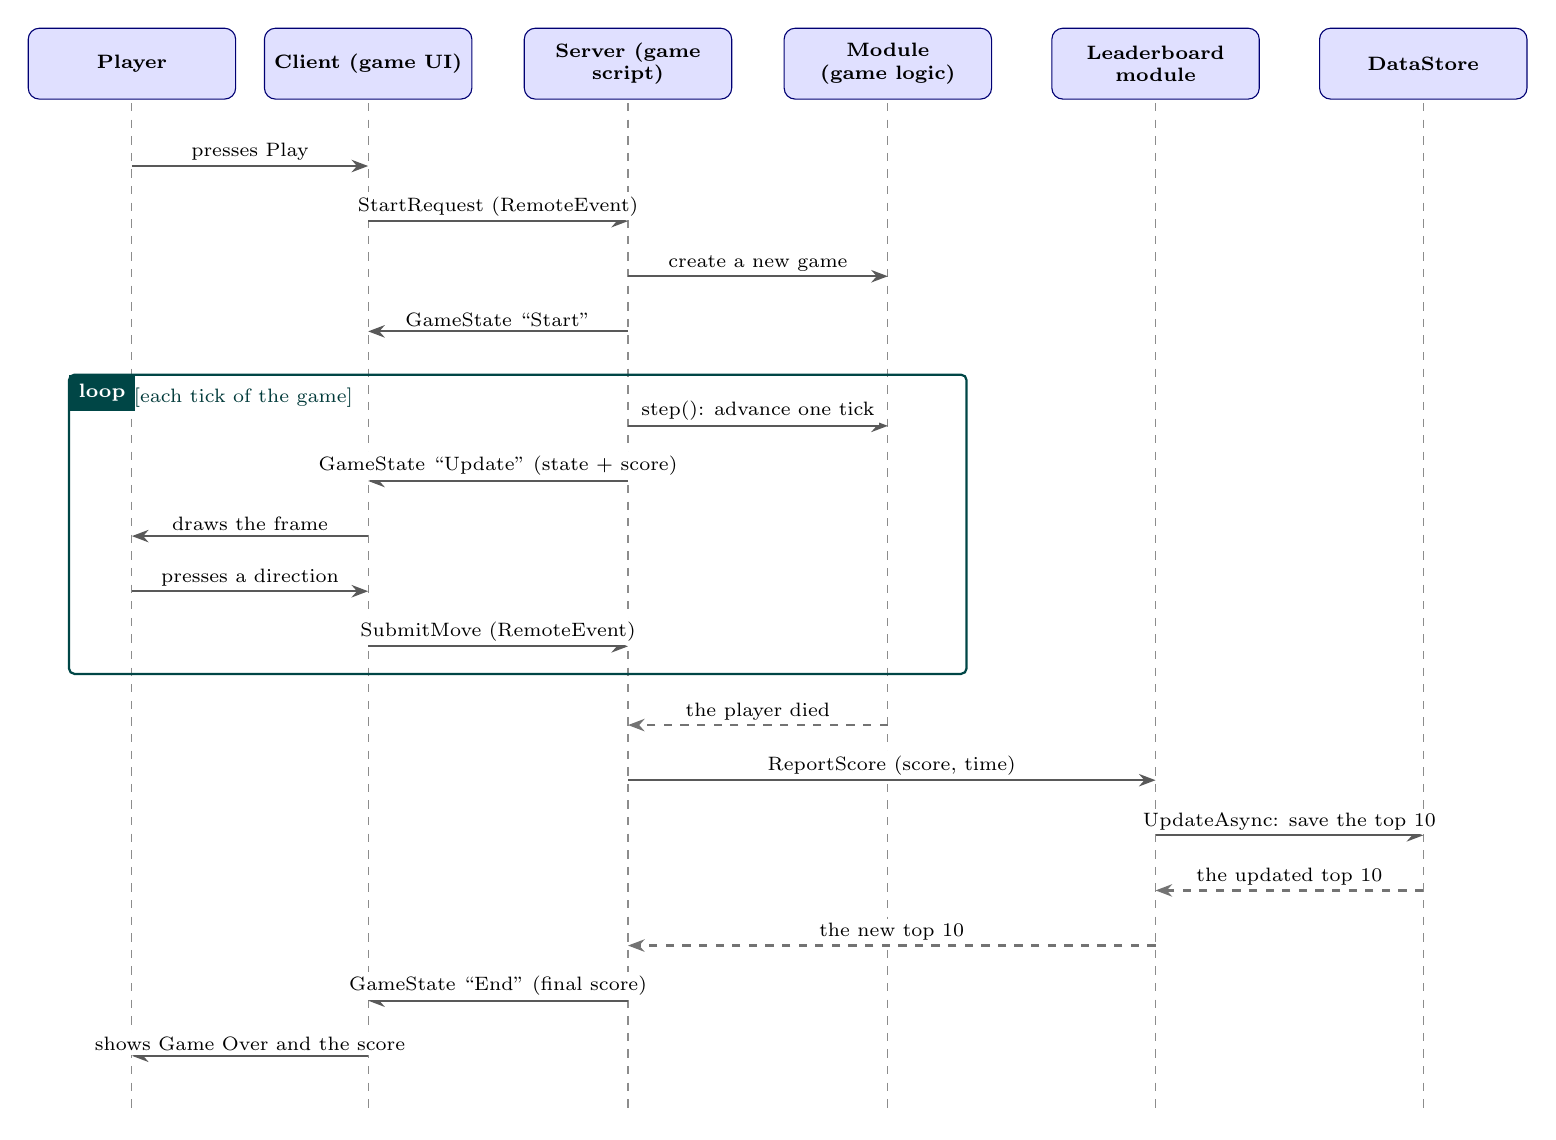
\begin{tikzpicture}[
  font=\small,
  >={Stealth[length=6pt]},
  party/.style={rectangle, rounded corners=4pt, draw=blue!45!black, fill=blue!12,
                align=center, font=\scriptsize\bfseries, minimum height=0.9cm, text width=2.4cm},
  life/.style={draw=black!45, dashed},
  msg/.style={->, thick, draw=black!65},
  ret/.style={->, thick, draw=black!55, dashed},
  ml/.style={font=\scriptsize, fill=white, inner sep=1.5pt, align=center},
]

\def\px{0}  \def\cx{3.0}  \def\sx{6.3}  \def\mx{9.6}  \def\lx{13.0}  \def\dx{16.4}
\def\bot{-13.3}

% participants
\node[party] (p) at (\px,0) {Player};
\node[party] (c) at (\cx,0) {Client (game UI)};
\node[party] (s) at (\sx,0) {Server (game script)};
\node[party] (m) at (\mx,0) {Module (game logic)};
\node[party] (l) at (\lx,0) {Leaderboard module};
\node[party] (d) at (\dx,0) {DataStore};

% lifelines
\foreach \x in {\px,\cx,\sx,\mx,\lx,\dx} { \draw[life] (\x,-0.5) -- (\x,\bot); }

% --- start ---
\draw[msg] (\px,-1.3) -- node[ml, above]{presses Play} (\cx,-1.3);
\draw[msg] (\cx,-2.0) -- node[ml, above]{StartRequest (RemoteEvent)} (\sx,-2.0);
\draw[msg] (\sx,-2.7) -- node[ml, above]{create a new game} (\mx,-2.7);
\draw[msg] (\sx,-3.4) -- node[ml, above]{GameState ``Start''} (\cx,-3.4);

% --- game loop frame ---
\draw[draw=teal!55!black, thick, rounded corners=2pt] (\px-0.8,-3.95) rectangle (\mx+1.0,-7.75);
\node[fill=teal!55!black, text=white, font=\scriptsize\bfseries, anchor=north west] at (\px-0.8,-3.95) {loop};
\node[font=\scriptsize, anchor=north west, text=teal!45!black] at (\px-0.1,-4.0) {[each tick of the game]};

\draw[msg] (\sx,-4.6) -- node[ml, above]{step(): advance one tick} (\mx,-4.6);
\draw[msg] (\sx,-5.3) -- node[ml, above]{GameState ``Update'' (state + score)} (\cx,-5.3);
\draw[msg] (\cx,-6.0) -- node[ml, above]{draws the frame} (\px,-6.0);
\draw[msg] (\px,-6.7) -- node[ml, above]{presses a direction} (\cx,-6.7);
\draw[msg] (\cx,-7.4) -- node[ml, above]{SubmitMove (RemoteEvent)} (\sx,-7.4);

% --- game over ---
\draw[ret] (\mx,-8.4) -- node[ml, above]{the player died} (\sx,-8.4);
\draw[msg] (\sx,-9.1) -- node[ml, above]{ReportScore (score, time)} (\lx,-9.1);
\draw[msg] (\lx,-9.8) -- node[ml, above]{UpdateAsync: save the top 10} (\dx,-9.8);
\draw[ret] (\dx,-10.5) -- node[ml, above]{the updated top 10} (\lx,-10.5);
\draw[ret] (\lx,-11.2) -- node[ml, above]{the new top 10} (\sx,-11.2);
\draw[msg] (\sx,-11.9) -- node[ml, above]{GameState ``End'' (final score)} (\cx,-11.9);
\draw[msg] (\cx,-12.6) -- node[ml, above]{shows Game Over and the score} (\px,-12.6);

\end{tikzpicture}
}
  \caption{Sequence diagram of a normal game session, showing the back and forth between the player, the client, the server, the game module, the leaderboard, and the DataStore.}
  \label{fig:sequence_session}
\end{figure}

Inside the ``Playing'' part of that flow, each round also moves through a small set of internal states. The flowcharts in each game focus on the rules, so the state machine below shows the technical side: the real states the code uses to manage a round, from the first countdown to game over, including losing a life and moving to the next level.

\begin{figure}[H]
  \centering
  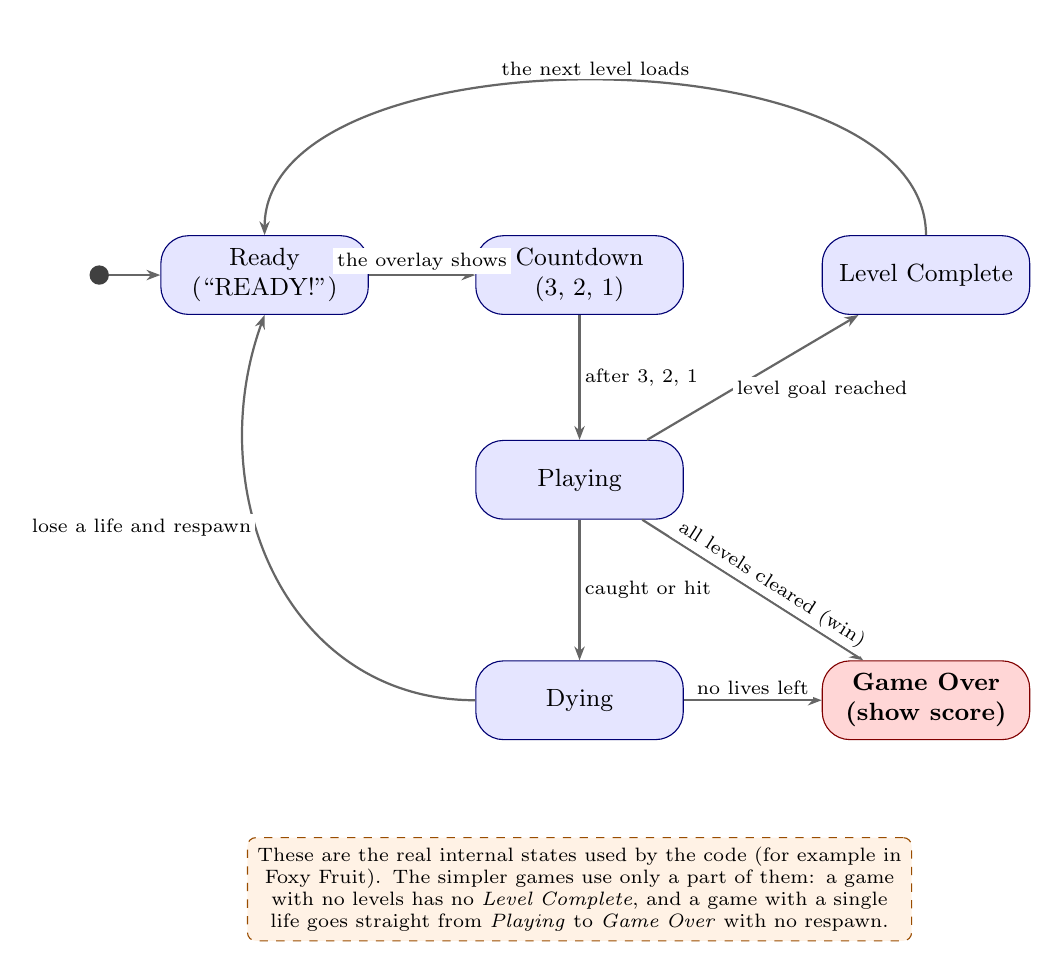
\begin{tikzpicture}[
  font=\small,
  >={Stealth[length=5pt]},
  state/.style={rectangle, rounded corners=10pt, draw=blue!45!black, fill=blue!10,
                text width=2.4cm, align=center, minimum height=1.0cm, font=\small},
  over/.style={rectangle, rounded corners=10pt, draw=red!50!black, fill=red!16,
               text width=2.4cm, align=center, minimum height=1.0cm, font=\small\bfseries},
  ini/.style={circle, fill=black!75, minimum size=7pt, inner sep=0},
  note/.style={rectangle, rounded corners=3pt, draw=orange!60!black, fill=orange!10, dashed,
               text width=8.2cm, align=center, font=\scriptsize},
  tr/.style={->, thick, draw=black!60},
  trlbl/.style={font=\scriptsize, fill=white, inner sep=1.5pt, align=center},
]

\node[ini]   (i)     at (-2.1,2.6) {};
\node[state] (ready) at (0,2.6)    {Ready (``READY!'')};
\node[state] (count) at (4.0,2.6)  {Countdown (3, 2, 1)};
\node[state] (play)  at (4.0,0)    {Playing};
\node[state] (level) at (8.4,2.6)  {Level Complete};
\node[state] (dying) at (4.0,-2.8) {Dying};
\node[over]  (over)  at (8.4,-2.8) {Game Over (show score)};

\draw[tr] (i) -- (ready);
\draw[tr] (ready) -- node[trlbl, above]{the overlay shows} (count);
\draw[tr] (count) -- node[trlbl, right]{after 3, 2, 1} (play);
\draw[tr] (play) -- node[trlbl, pos=0.4, right]{level goal reached} (level);
\draw[tr] (level.north) to[out=90, in=90, looseness=0.8]
  node[trlbl, above]{the next level loads} (ready.north);
\draw[tr] (play) -- node[trlbl, right]{caught or hit} (dying);
\draw[tr] (dying.west) to[out=180, in=250, looseness=1.1]
  node[trlbl, left, pos=0.6]{lose a life and respawn} (ready.south);
\draw[tr] (dying) -- node[trlbl, above]{no lives left} (over);
\draw[tr] (play) -- node[trlbl, pos=0.55, above, sloped]{all levels cleared (win)} (over);

\node[note] (n) at (4.0,-5.2)
  {These are the real internal states used by the code (for example in Foxy Fruit). The simpler games use only a part of them: a game with no levels has no \emph{Level Complete}, and a game with a single life goes straight from \emph{Playing} to \emph{Game Over} with no respawn.};

\end{tikzpicture}

  \caption{Internal state machine of a single round. These are the real states from the code; simpler games use only a part of them.}
  \label{fig:round_states}
\end{figure}

\clearpage

\subsection{Oxybelis}

Oxybelis is a grid based arcade game built from scratch inside Roblox Studio. The idea is simple: guide a growing creature around a closed grid without crashing into the walls or into its own body. The project took five days. The first two days went into learning Roblox Studio and getting the movement to feel right, and the last three went into the global leaderboard, which turned out to be the hardest part. It was hard not because of the sorting, but because of the DataStore rate limits and making sure no score was ever lost if the server crashed.

\subsubsection{Rules of Oxybelis}
\begin{itemize}
  \item \textbf{Main Goal:} Eat as much food as possible without crashing.
  \item \textbf{Controls (PC):} Arrow keys or WASD for direction. The game is also adapted for mobile touchscreen, Xbox, and PlayStation controllers through \texttt{UniversalController}.
  \item \textbf{Core Mechanics:}
  \begin{itemize}
    \item The creature moves on its own at a fixed speed; the player only chooses the direction.
    \item Food appears on a random free cell. Eating it makes the body one cell longer and adds one to the score.
  \end{itemize}
  \item \textbf{End Conditions:} The game ends when the creature hits a wall or its own body. A perfect game happens when the body fills the whole $16 \times 12$ grid.
\end{itemize}

\textbf{Flowchart}
\begin{figure}[H]
  \centering
  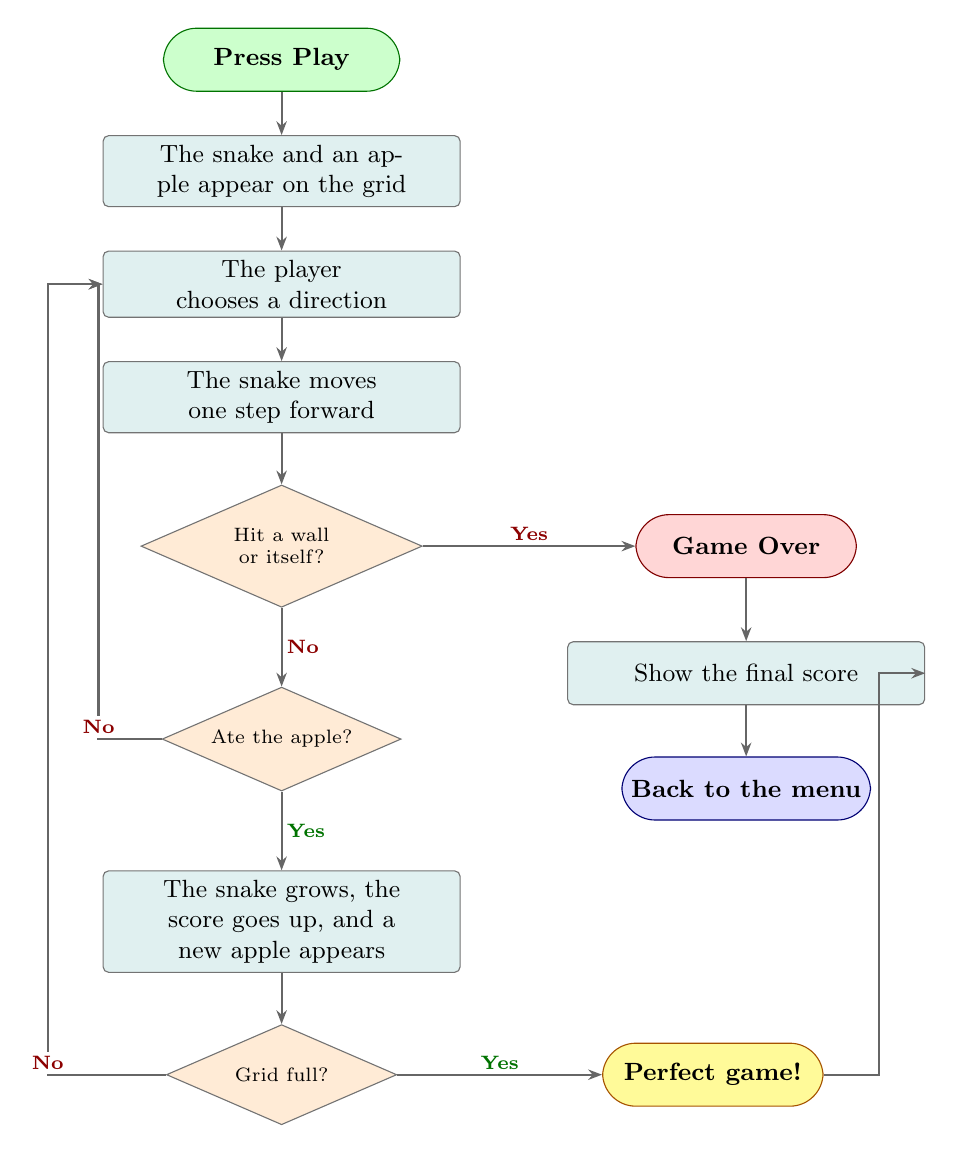
\begin{tikzpicture}[
  font=\small,
  >={Stealth[length=5pt]},
  start/.style={rectangle, rounded corners=12pt, draw=green!45!black, fill=green!20,
                minimum width=3cm, minimum height=0.8cm, align=center, font=\small\bfseries},
  menu/.style={rectangle, rounded corners=12pt, draw=blue!45!black, fill=blue!14,
               minimum width=3cm, minimum height=0.8cm, align=center, font=\small\bfseries},
  over/.style={rectangle, rounded corners=12pt, draw=red!50!black, fill=red!16,
               minimum width=2.8cm, minimum height=0.8cm, align=center, font=\small\bfseries},
  win/.style={rectangle, rounded corners=12pt, draw=orange!65!black, fill=yellow!40,
              minimum width=2.8cm, minimum height=0.8cm, align=center, font=\small\bfseries},
  act/.style={rectangle, draw=black!55, fill=teal!12, rounded corners=2pt,
              text width=4.3cm, minimum height=0.8cm, align=center},
  dec/.style={diamond, draw=black!55, fill=orange!16, aspect=2.3,
              align=center, inner sep=1pt, text width=2.3cm, font=\scriptsize},
  link/.style={->, thick, draw=black!60},
  yeslbl/.style={font=\scriptsize\bfseries, color=green!45!black, fill=white, inner sep=1.5pt},
  nolbl/.style={font=\scriptsize\bfseries, color=red!55!black, fill=white, inner sep=1.5pt},
]

% main column
\node[start] (s) {Press Play};
\node[act, below=0.55cm of s]     (init)  {The snake and an apple appear on the grid};
\node[act, below=0.55cm of init]  (move)  {The player chooses a direction};
\node[act, below=0.55cm of move]  (adv)   {The snake moves one step forward};
\node[dec, below=0.65cm of adv]   (crash) {Hit a wall or itself?};
\node[dec, below=1.0cm of crash]  (eat)   {Ate the apple?};
\node[act, below=1.0cm of eat]    (grow)  {The snake grows, the score goes up, and a new apple appears};
\node[dec, below=0.65cm of grow]  (full)  {Grid full?};

% right exit column
\node[over,  right=2.7cm of crash] (go)    {Game Over};
\node[act,   below=0.8cm of go]    (score) {Show the final score};
\node[menu,  below=0.65cm of score](back)  {Back to the menu};

% win node
\node[win, right=2.6cm of full] (perfect) {Perfect game!};

% main flow
\draw[link] (s)    -- (init);
\draw[link] (init) -- (move);
\draw[link] (move) -- (adv);
\draw[link] (adv)  -- (crash);
\draw[link] (crash) -- node[nolbl, right]{No} (eat);
\draw[link] (eat)   -- node[yeslbl, right]{Yes} (grow);
\draw[link] (grow)  -- (full);

% crash yes -> game over
\draw[link] (crash.east) -- node[nolbl, above]{Yes} (go.west);

% game over chain
\draw[link] (go)    -- (score);
\draw[link] (score) -- (back);

% full yes -> perfect game -> show score
\draw[link] (full.east) -- node[yeslbl, above]{Yes} (perfect.west);
\draw[link] (perfect.east) -- ++(0.7,0) |- (score.east);

% loop backs to "choose a direction"
\draw[link] (eat.west)  -- ++(-0.8,0) node[nolbl, above]{No}  |- (move.west);
\draw[link] (full.west) -- ++(-1.5,0) node[nolbl, above]{No}  |- (move.west);

\end{tikzpicture}

  \caption{Flowchart for Oxybelis.}
  \label{fig:oxybelis_flow}
\end{figure}

\subsubsection{Project Structure}

Oxybelis is split across four files that follow the way Roblox separates the client and the server. Each file has one clear job.

\begin{lstlisting}
Oxybelis/
|-- Workspace/
|   +-- Oxybelis/ (Folder)
|       +-- ButtonOxybelis      (Part, Tag="ButtonOxybelis")
|-- ReplicatedStorage/
|   |-- ArcadeRemotes/
|   |   +-- Oxybelis/ (Folder)
|   |       |-- StartRequest    (RemoteEvent)
|   |       |-- SubmitMove      (RemoteEvent)
|   |       |-- GameState       (RemoteEvent)
|   |       +-- ToggleAudio     (RemoteEvent)
|   +-- Modules/
|       +-- OxybelisModule      (ModuleScript)
|-- ServerScriptService/
|   +-- OxybelisServer          (Script)
+-- StarterPlayer/
    +-- StarterPlayerScripts/
        +-- OxybelisClient      (LocalScript)
\end{lstlisting}


\subsubsection{Time Complexity}
Each game tick is very cheap to run, with a cost of $O(1)$. The \texttt{step()} function moves the creature by shifting two pointers in a circular buffer, checks the walls with simple number comparisons, and checks whether the head touched the body by looking it up in a table. All of these take the same small amount of time, no matter how long the creature is. Placing new food is also $O(1)$, because the game keeps a list of free cells and picks one at random instead of scanning the whole grid. The only part that grows with the creature is \texttt{getOxybelis()}, which copies the body into a list to send to the screen; this costs $O(L)$, where $L$ is the current length. Since the body can never be longer than the grid ($16 \times 12 = 192$ cells), even this stays small. In short, the game stays fast no matter how big the creature gets.

\subsubsection{Space Complexity}
The memory the game uses stays fixed at $O(N)$, where $N = 192$ is the number of cells. Four structures are created when the game starts and never grow: the circular buffer that holds the body, a table that marks which cells are taken, and two lists that keep track of the free cells. Nothing new is created while playing. A cell simply goes back to the free list when the tail moves, and is taken again when the body grows. Because of this, the memory stays the same from the first second to the last, no matter the score or the length of the creature.

\subsubsection{Game Features and Implementation Status}

\begin{table}[H]
\centering
\begin{tabular}{|p{4cm}|p{8cm}|p{2.5cm}|}
\hline
\textbf{Feature} & \textbf{Description} & \textbf{Status} \\
\hline
Main Menu & Interface with Play, VIP, and Exit buttons. Supports navigation via A, S, arrow keys, and selection with Space/Enter. & Working \\
\hline
Menu Sounds & UI elements include audio feedback for navigation and selection. & Working \\
\hline
Gameplay Movement & Responsive control system using WASD or arrow keys. & Working \\
\hline
Mute Button & In game toggle to turn all audio on or off. & Working \\
\hline
Exit Button (Game) & Allows the player to abort the run and return to the score menu. & Working \\
\hline
Score Menu & Post game screen displaying the final score and options to replay or exit. & Working \\
\hline
Top 10 Score Table & Displays the top 10 players globally. Uses Roblox DataStore for persistent online storage. & Working \\
\hline
VIP Donation Menu & Opens a menu with various donation tiers using in game currency. & Working \\
\hline
Optimization & Circular buffer implementation ensures $O(1)$ logic updates. & Working \\
\hline
Mobile Adaptation & Touchscreen controls and UI scaling via UniversalController. & Working \\
\hline
Xbox Adaptation & Gamepad support and console UI via UniversalController. & Working \\
\hline
PlayStation Adaptation & DualSense and DualShock input support via UniversalController. & Working \\
\hline
\end{tabular}
\caption{Functionalities and current status of Oxybelis.}
\end{table}

\subsubsection{Game Results}
The following images illustrate the final implementation, including the user interface, gameplay view, and score summary.

\begin{figure}[H]
    \centering
    \begin{minipage}[b]{0.32\textwidth}
        \centering
        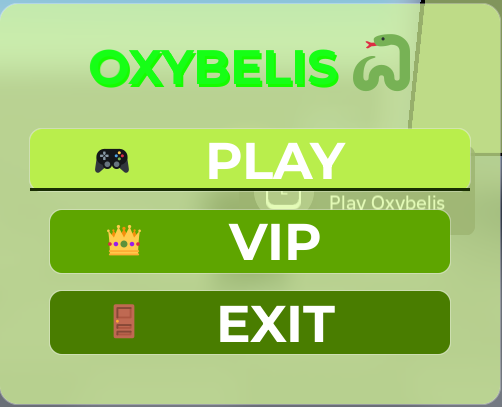
\includegraphics[width=\linewidth]{desarrollo/mo1.png}
        \caption*{\textbf{Main Menu:} Features animated buttons and sound effects.}
    \end{minipage}
    \hfill
    \begin{minipage}[b]{0.32\textwidth}
        \centering
        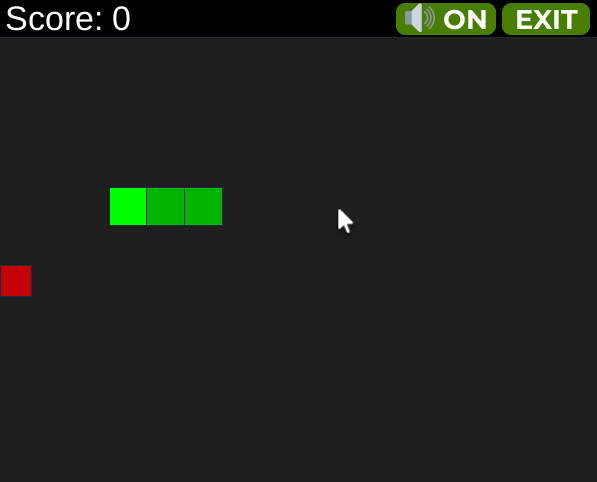
\includegraphics[width=\linewidth]{desarrollo/mo2.png}
        \caption*{\textbf{Gameplay:} The active game state with HUD elements.}
    \end{minipage}
    \hfill
    \begin{minipage}[b]{0.32\textwidth}
        \centering
        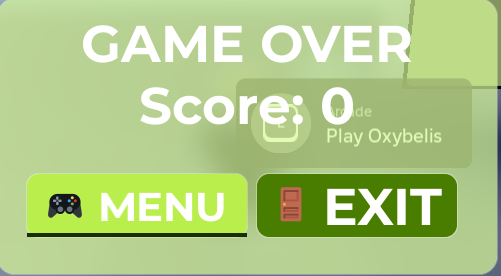
\includegraphics[width=\linewidth]{desarrollo/mo3.png}
        \caption*{\textbf{Score Menu:} Post game summary and navigation.}
    \end{minipage}
\end{figure}

\subsubsection{VIP and Global Scores}
The project includes a monetization test via a VIP donation system and a competitive leaderboard managed via the cloud.

\begin{figure}[H]
    \centering
    \begin{minipage}[b]{0.47\textwidth}
        \centering
        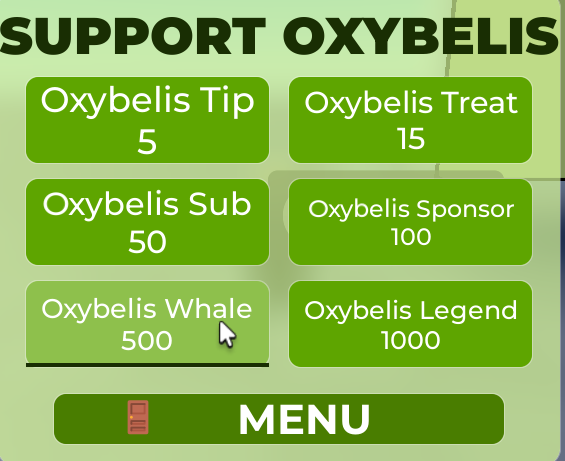
\includegraphics[width=\linewidth]{desarrollo/mo4.png}
        \caption*{\textbf{VIP Section:} Donation menu interface.}
    \end{minipage}
    \hfill
    \begin{minipage}[b]{0.47\textwidth}
        \centering
        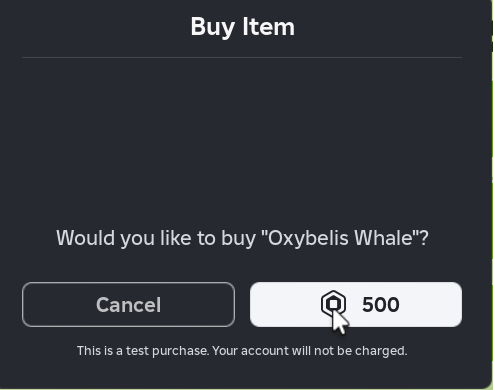
\includegraphics[width=\linewidth]{desarrollo/mo5.png}
        \caption*{\textbf{Donation Process:} Transaction confirmation flow.}
    \end{minipage}
\end{figure}

\begin{figure}[H]
    \centering
    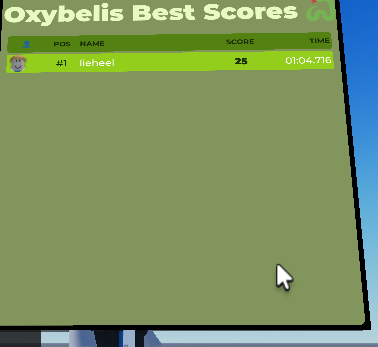
\includegraphics[width=0.6\textwidth]{desarrollo/mo6.png}
    \caption*{\textbf{Global Score Table:} Displays the top 10 players. Ties are resolved by comparing completion time.}
\end{figure}

\clearpage

\subsection{Avis Toucan}

Avis Toucan is a side scrolling arcade game built inside Roblox Studio. The goal is simple: keep the bird in the air as long as possible by tapping at the right moments to pass through the gaps between the pipes. The project took four days. The logic itself was not the hard part, since gravity, collision, and spawning pipes are each only a few lines. The real challenge was the game feel: adjusting the gravity (900\,px/s\textsuperscript{2}) and the flap force ($-320$\,px/s) until the difficulty felt fair without being frustrating, especially for a younger audience.

\subsubsection{Rules of Avis Toucan}
\begin{itemize}
  \item \textbf{Main Goal:} Navigate through pipe gaps to achieve the highest score.
  \item \textbf{Controls (PC):} Click or press Space to flap. Also adapted for mobile touchscreen, Xbox, and PlayStation controllers via \texttt{UniversalController}.
  \item \textbf{Core Mechanics:} The bird is subject to continuous gravity (900\,px/s\textsuperscript{2}). Each flap applies an upward velocity impulse of $-320$\,px/s. Pipes spawn every 1.8\,s and move left at 117\,px/s.
  \item \textbf{Scoring:} One point for every pipe pair cleared.
  \item \textbf{End Condition:} Hitting a pipe or the ground ends the session immediately.
\end{itemize}

\textbf{Flowchart}
\begin{figure}[H]
  \centering
  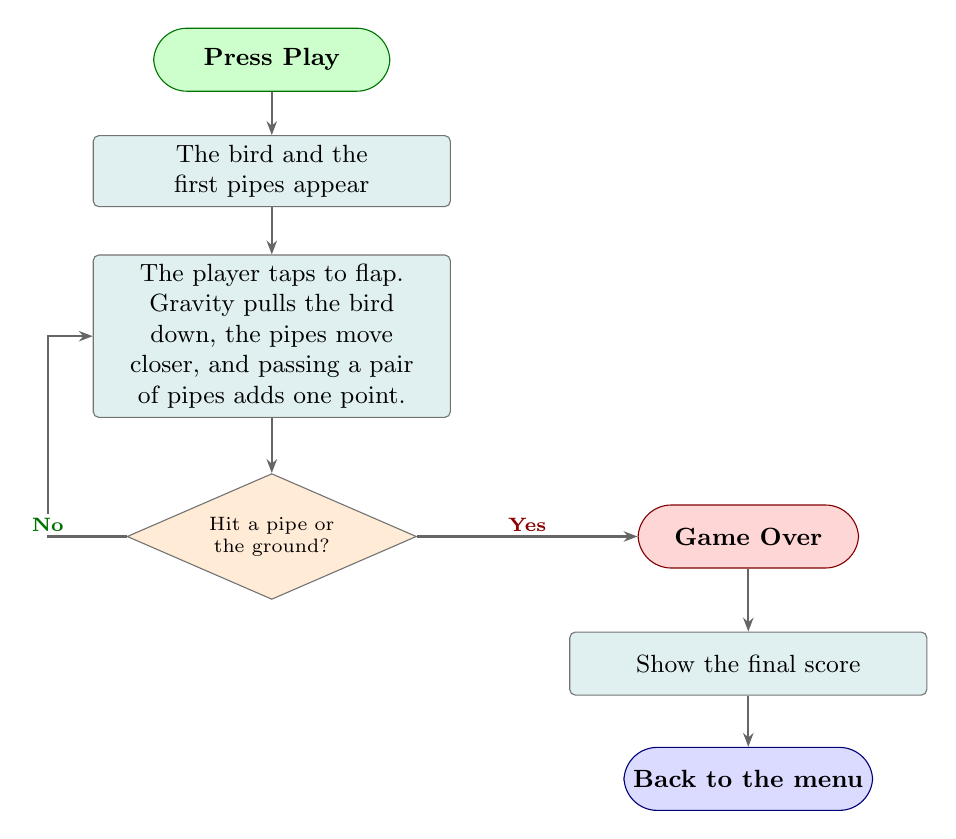
\begin{tikzpicture}[
  font=\small,
  >={Stealth[length=5pt]},
  start/.style={rectangle, rounded corners=12pt, draw=green!45!black, fill=green!20,
                minimum width=3cm, minimum height=0.8cm, align=center, font=\small\bfseries},
  menu/.style={rectangle, rounded corners=12pt, draw=blue!45!black, fill=blue!14,
               minimum width=3cm, minimum height=0.8cm, align=center, font=\small\bfseries},
  over/.style={rectangle, rounded corners=12pt, draw=red!50!black, fill=red!16,
               minimum width=2.8cm, minimum height=0.8cm, align=center, font=\small\bfseries},
  win/.style={rectangle, rounded corners=12pt, draw=orange!65!black, fill=yellow!40,
              minimum width=2.8cm, minimum height=0.8cm, align=center, font=\small\bfseries},
  act/.style={rectangle, draw=black!55, fill=teal!12, rounded corners=2pt,
              text width=4.3cm, minimum height=0.8cm, align=center},
  dec/.style={diamond, draw=black!55, fill=orange!16, aspect=2.3,
              align=center, inner sep=1pt, text width=2.3cm, font=\scriptsize},
  link/.style={->, thick, draw=black!60},
  yeslbl/.style={font=\scriptsize\bfseries, color=green!45!black, fill=white, inner sep=1.5pt},
  nolbl/.style={font=\scriptsize\bfseries, color=red!55!black, fill=white, inner sep=1.5pt},
]

\node[start] (s) {Press Play};
\node[act, below=0.55cm of s]    (init) {The bird and the first pipes appear};
\node[act, below=0.6cm of init]  (play) {The player taps to flap. Gravity pulls the bird down, the pipes move closer, and passing a pair of pipes adds one point.};
\node[dec, below=0.7cm of play]  (hit)  {Hit a pipe or the ground?};
\node[over, right=2.8cm of hit]  (go)   {Game Over};
\node[act, below=0.8cm of go]    (score){Show the final score};
\node[menu, below=0.65cm of score](back){Back to the menu};

\draw[link] (s) -- (init);
\draw[link] (init) -- (play);
\draw[link] (play) -- (hit);
\draw[link] (hit.east) -- node[nolbl, above]{Yes} (go.west);
\draw[link] (hit.west) -- ++(-1.0,0) node[yeslbl, above]{No} |- (play.west);
\draw[link] (go) -- (score);
\draw[link] (score) -- (back);

\end{tikzpicture}

  \caption{Flowchart for Avis Toucan.}
  \label{fig:avistoucan_flow}
\end{figure}

\subsubsection{Project Structure}

Avis Toucan follows the same four file layout as the rest of the arcade. Each component has one clear responsibility and no cross game dependencies.

\begin{lstlisting}
AvisToucan/
|-- Workspace/
|   +-- AvisToucan/ (Folder)
|       +-- ButtonAvisToucan   (Part, Tag="ButtonAvisToucan")
|-- ReplicatedStorage/
|   |-- ArcadeRemotes/
|   |   +-- AvisToucan/ (Folder)
|   |       |-- StartAvisToucanRequest  (RemoteEvent)
|   |       |-- SubmitFlap              (RemoteEvent)
|   |       |-- GameState               (RemoteEvent)
|   |       +-- ToggleAudio             (RemoteEvent)
|   +-- Modules/
|       +-- AvisToucanModule   (ModuleScript)
|-- ServerScriptService/
|   +-- AvisToucanServer       (Script)
+-- StarterPlayer/
    +-- StarterPlayerScripts/
        +-- AvisToucanClient   (LocalScript)
\end{lstlisting}


\subsubsection{Time Complexity}

Each call to \texttt{step(dt)} costs $O(P)$ time, where $P$ is the number of pipes on screen. Moving the bird and applying gravity are $O(1)$. Moving the pipes, removing the ones that have left the screen, and checking for collisions all go through the list of pipes, which is what gives the $O(P)$. The key point is that there are never many pipes at once: since a new pipe appears every 1.8 seconds and they move at 117 pixels per second across a screen 480 pixels wide, at most 3 pipes can be visible at the same time. With $P$ always 3 or fewer, the real cost per tick is basically $O(1)$. Sending the game state to the screen is also $O(P)$ and happens every 50 milliseconds.

\subsubsection{Space Complexity}

The memory cost is $O(P)$, where $P$ is at most 3 pipes. The only thing that grows while playing is the list of pipes, and a pipe is removed as soon as it leaves the left edge, so the list never piles up. Everything else (the bird's position and speed, the score, the spawn timer) is a single value. In practice, the memory used in a session stays constant.

\subsubsection{Game Features and Implementation Status}

\begin{table}[H]
\centering
\begin{tabular}{|p{4cm}|p{8cm}|p{2.5cm}|}
\hline
\textbf{Feature} & \textbf{Description} & \textbf{Status} \\
\hline
Main Menu & Interface with Play, VIP, and Exit buttons. & Working \\
\hline
Menu Sounds & Audio feedback for navigation and selection. & Working \\
\hline
Gameplay Control & One button control (click, tap, or Space). & Working \\
\hline
Mute Button & In game toggle to turn all audio on or off. & Working \\
\hline
Exit Button (Game) & Allows the player to abort the run and return to the score menu. & Working \\
\hline
Score Menu & A screen after the game showing the final score and a replay option. & Working \\
\hline
Top 10 Score Table & Global leaderboard via Roblox DataStore. & Working \\
\hline
VIP Donation Menu & Opens a menu with various donation tiers. & Working \\
\hline
Optimization & $dt$-based physics integration; pipe count bounded at $P \leq 3$, giving $O(1)$ practical cost per tick. & Working \\
\hline
Mobile Adaptation & Touchscreen tap input via \texttt{UniversalController}. & Working \\
\hline
Xbox Adaptation & Gamepad button input via \texttt{UniversalController}. & Working \\
\hline
PlayStation Adaptation & DualSense and DualShock input via \texttt{UniversalController}. & Working \\
\hline
\end{tabular}
\caption{Functionalities and current status of Avis Toucan.}
\end{table}

\subsubsection{Game Results}

\begin{figure}[H]
    \centering
    \begin{minipage}[b]{0.32\textwidth}
        \centering
        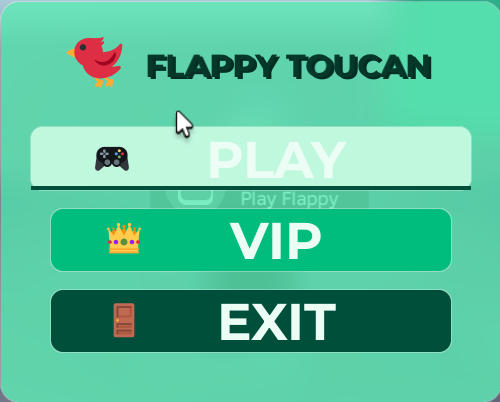
\includegraphics[width=\linewidth]{desarrollo/Fm1.png}
        \caption*{\textbf{Main Menu}}
    \end{minipage}
    \hfill
    \begin{minipage}[b]{0.32\textwidth}
        \centering
        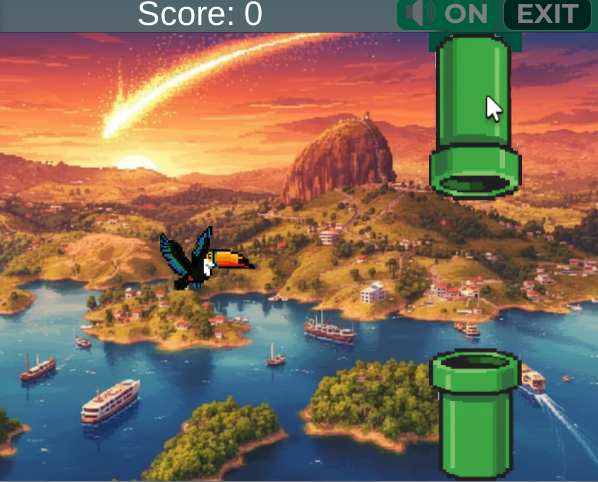
\includegraphics[width=\linewidth]{desarrollo/Fm2.png}
        \caption*{\textbf{Gameplay}}
    \end{minipage}
    \hfill
    \begin{minipage}[b]{0.32\textwidth}
        \centering
        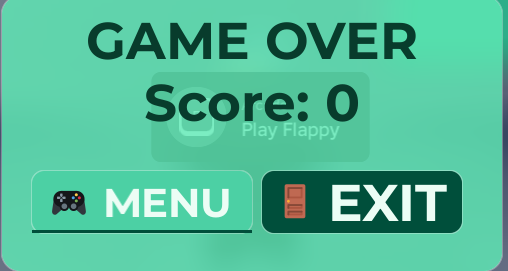
\includegraphics[width=\linewidth]{desarrollo/Fm3.png}
        \caption*{\textbf{Score Menu}}
    \end{minipage}
\end{figure}

\begin{figure}[H]
    \centering
    \begin{minipage}[b]{0.47\textwidth}
        \centering
        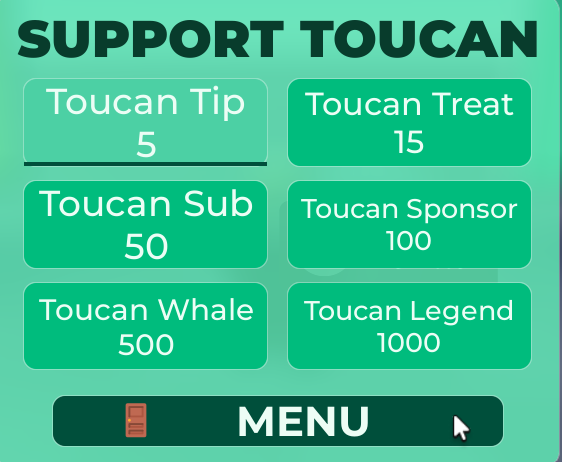
\includegraphics[width=\linewidth]{desarrollo/Fm4.png}
        \caption*{\textbf{VIP Menu}}
    \end{minipage}
    \hfill
    \begin{minipage}[b]{0.47\textwidth}
        \centering
        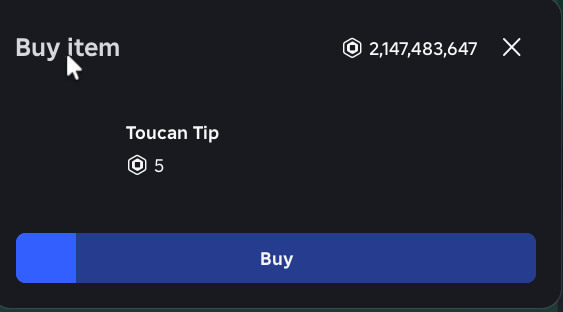
\includegraphics[width=\linewidth]{desarrollo/Fm5.png}
        \caption*{\textbf{Donation System}}
    \end{minipage}
\end{figure}

\begin{figure}[H]
    \centering
    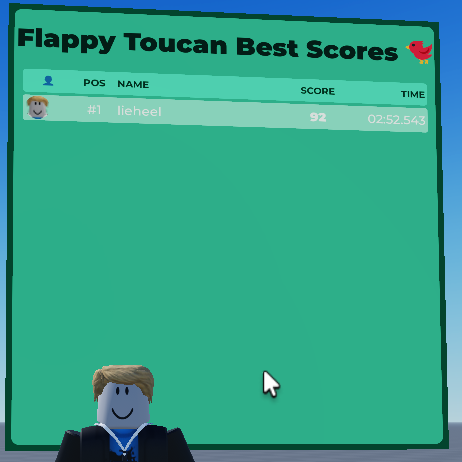
\includegraphics[width=0.6\textwidth]{desarrollo/Fm6.png}
    \caption*{\textbf{Global Score Table:} Top 10 ranking.}
\end{figure}

\clearpage

\subsection{Resilio}

Resilio is a ball and paddle arcade game built inside Roblox Studio. It had two main challenges. The first was the physics: the ball bounces off the paddle at an angle that depends on where it lands, it collides with the bricks, and some bricks need more than one hit to break. The second was the system of levels, with five handmade layouts that the player clears one by one. The game also adds an auto fire power up, dropped by a special brick, that gives the paddle laser shots for four seconds and brings a bit of strategy to the usual gameplay.

\subsubsection{Rules of Resilio}
\begin{itemize}
  \item \textbf{Main Goal:} Destroy all bricks across five levels without losing all three lives.
  \item \textbf{Controls (PC):} Arrow keys or A/D to move the paddle, Space to launch the ball. Also adapted for mobile touchscreen, Xbox, and PlayStation controllers via \texttt{UniversalController}.
  \item \textbf{Mechanics:} The ball reflects off walls and the paddle. The deflection angle is calculated from the impact position on the paddle, clamped to $\pm60°$. Ball speed increases by 10\,px/s on each paddle hit, up to a maximum of 250\,px/s.
  \item \textbf{Bricks:} Three brick types (normal, medium, hard). At level load, 5 to 10 random bricks are assigned 2 to 4 HP. One of them is the auto fire brick worth 50 points.
  \item \textbf{Auto fire:} Destroying the special brick activates 4 seconds of laser fire from the paddle, targeting the nearest brick every 125\,ms.
  \item \textbf{Lives:} The session starts with 3 lives. Clearing a level grants 1 extra life.
  \item \textbf{End Condition:} Losing all lives ends the session. Clearing all five levels triggers a perfect game.
\end{itemize}

\textbf{Flowchart}
\begin{figure}[H]
  \centering
  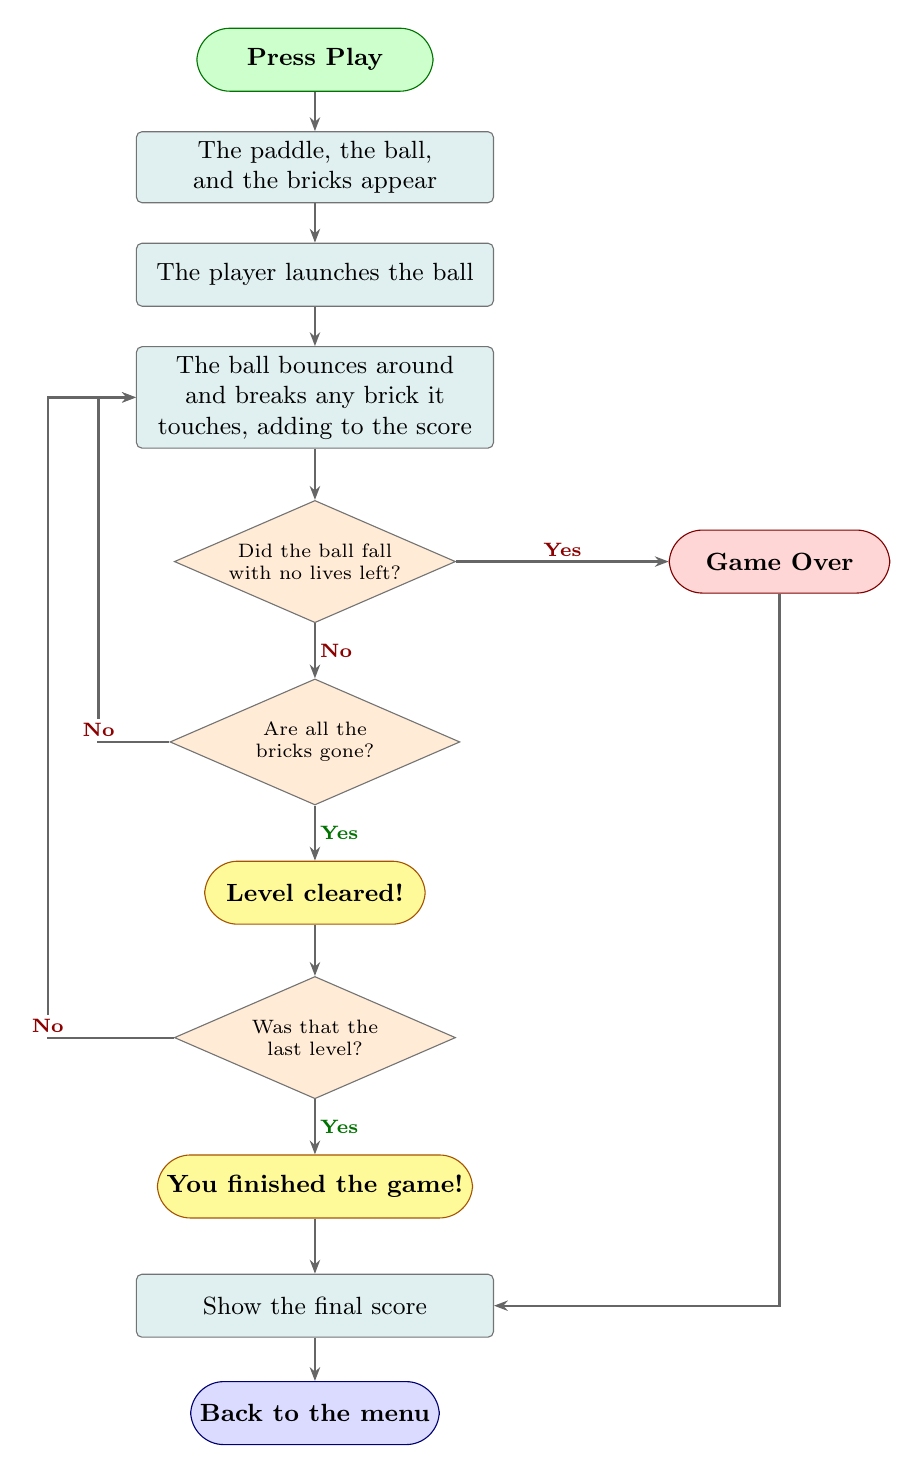
\begin{tikzpicture}[
  font=\small,
  >={Stealth[length=5pt]},
  start/.style={rectangle, rounded corners=12pt, draw=green!45!black, fill=green!20,
                minimum width=3cm, minimum height=0.8cm, align=center, font=\small\bfseries},
  menu/.style={rectangle, rounded corners=12pt, draw=blue!45!black, fill=blue!14,
               minimum width=3cm, minimum height=0.8cm, align=center, font=\small\bfseries},
  over/.style={rectangle, rounded corners=12pt, draw=red!50!black, fill=red!16,
               minimum width=2.8cm, minimum height=0.8cm, align=center, font=\small\bfseries},
  win/.style={rectangle, rounded corners=12pt, draw=orange!65!black, fill=yellow!40,
              minimum width=2.8cm, minimum height=0.8cm, align=center, font=\small\bfseries},
  act/.style={rectangle, draw=black!55, fill=teal!12, rounded corners=2pt,
              text width=4.3cm, minimum height=0.8cm, align=center},
  dec/.style={diamond, draw=black!55, fill=orange!16, aspect=2.3,
              align=center, inner sep=1pt, text width=2.3cm, font=\scriptsize},
  link/.style={->, thick, draw=black!60},
  yeslbl/.style={font=\scriptsize\bfseries, color=green!45!black, fill=white, inner sep=1.5pt},
  nolbl/.style={font=\scriptsize\bfseries, color=red!55!black, fill=white, inner sep=1.5pt},
]

\node[start] (s) {Press Play};
\node[act, below=0.5cm of s]      (init)   {The paddle, the ball, and the bricks appear};
\node[act, below=0.5cm of init]   (launch) {The player launches the ball};
\node[act, below=0.5cm of launch] (play)   {The ball bounces around and breaks any brick it touches, adding to the score};
\node[dec, below=0.65cm of play]  (lost)   {Did the ball fall with no lives left?};
\node[dec, below=0.7cm of lost]   (clear)  {Are all the bricks gone?};
\node[win, below=0.7cm of clear]  (cleared){Level cleared!};
\node[dec, below=0.65cm of cleared](last)  {Was that the last level?};
\node[win, below=0.7cm of last]   (finish) {You finished the game!};
\node[act, below=0.7cm of finish] (score)  {Show the final score};
\node[menu, below=0.55cm of score](back)   {Back to the menu};

\node[over, right=2.7cm of lost]  (go)     {Game Over};

\draw[link] (s) -- (init);
\draw[link] (init) -- (launch);
\draw[link] (launch) -- (play);
\draw[link] (play) -- (lost);
\draw[link] (lost) -- node[nolbl, right]{No} (clear);
\draw[link] (lost.east) -- node[nolbl, above]{Yes} (go.west);
\draw[link] (clear) -- node[yeslbl, right]{Yes} (cleared);
\draw[link] (cleared) -- (last);
\draw[link] (last) -- node[yeslbl, right]{Yes} (finish);
\draw[link] (finish) -- (score);
\draw[link] (score) -- (back);
\draw[link] (go) |- (score.east);
\draw[link] (clear.west) -- ++(-0.9,0) node[nolbl, above]{No} |- (play.west);
\draw[link] (last.west) -- ++(-1.6,0) node[nolbl, above]{No} |- (play.west);

\end{tikzpicture}

  \caption{Flowchart for Resilio.}
  \label{fig:resilio_flow}
\end{figure}

\subsubsection{Project Structure}

Resilio uses the same four file layout as the rest of the arcade.

\begin{lstlisting}
Resilio/
|-- Workspace/
|   +-- Resilio/ (Folder)
|       +-- ButtonResilio          (Part, Tag="ButtonResilio")
|-- ReplicatedStorage/
|   |-- ArcadeRemotes/
|   |   +-- Resilio/ (Folder)
|   |       |-- StartResilioRequest  (RemoteEvent)
|   |       |-- SubmitMoveInput      (RemoteEvent)
|   |       |-- SubmitLaunch         (RemoteEvent)
|   |       |-- GameState            (RemoteEvent)
|   |       +-- ToggleAudio          (RemoteEvent)
|   +-- Modules/
|       +-- ResilioModule          (ModuleScript)
|-- ServerScriptService/
|   +-- ResilioServer              (Script)
+-- StarterPlayer/
    +-- StarterPlayerScripts/
        +-- ResilioClient          (LocalScript)
\end{lstlisting}

\subsubsection{Time Complexity}

Each call to \texttt{step(dt)} costs $O(B)$ time, where $B$ is the number of bricks still standing. Moving the paddle is $O(1)$, and bouncing the ball off the walls and the paddle is $O(1)$ as well. Checking the ball against the bricks goes through the brick list once, which gives the $O(B)$, and the auto fire also looks through the bricks to find the nearest one, again $O(B)$. At the start of a level there are at most 120 bricks (12 columns and up to 10 rows), and that number only goes down as the player breaks them, so the game gets cheaper as the level goes on. Sending the state to the screen copies the live bricks in $O(B)$ and the active laser shots, which are never more than 2 at a time.

\subsubsection{Space Complexity}

The memory cost is $O(B)$, where $B$ is at most 120 bricks per level. Each brick keeps its position, size, hit points, type, and a flag for the special brick. When a brick is broken it is simply marked as not alive and left out of the state sent to the screen; the game keeps a separate counter that reaches zero when the level is cleared. The laser shots are kept in a small list that never holds more than 2 at once. Everything else (the paddle, the ball, the lives, the score, the current level) is a single value.

\subsubsection{Game Features and Implementation Status}

\begin{table}[H]
\centering
\begin{tabular}{|p{4cm}|p{8cm}|p{2.5cm}|}
\hline
\textbf{Feature} & \textbf{Description} & \textbf{Status} \\
\hline
Main Menu & Interface with Play, VIP, and Exit buttons. & Working \\
\hline
Menu Sounds & Audio feedback for navigation and selection. & Working \\
\hline
Gameplay Controls & Paddle movement (left/right) and ball launch. & Working \\
\hline
Mute Button & In game toggle to turn all audio on or off. & Working \\
\hline
Exit Button (Game) & Allows the player to abort the run and return to the score menu. & Working \\
\hline
Score Menu & A screen after the game showing the final score and a replay option. & Working \\
\hline
Level System & Five built in layouts with increasing complexity. Clearing a level grants 1 extra life. & Working \\
\hline
Multi HP Brick System & Bricks have 1 to 4 HP. Tough bricks are assigned randomly at level load. & Working \\
\hline
Auto fire Power up & Destroying the special brick activates 4\,s of laser shots from the paddle, targeting the nearest brick every 125\,ms. & Working \\
\hline
Top 10 Score Table & Global leaderboard via Roblox DataStore. & Working \\
\hline
VIP Donation Menu & Opens a menu with various donation tiers. & Working \\
\hline
Optimization & $O(B)$ collision scan with $B$ decreasing per level; $S \leq 2$ active shots at any instant. & Working \\
\hline
Mobile Adaptation & Touchscreen input via \texttt{UniversalController}. & Working \\
\hline
Xbox Adaptation & Gamepad input via \texttt{UniversalController}. & Working \\
\hline
PlayStation Adaptation & DualSense and DualShock input via \texttt{UniversalController}. & Working \\
\hline
\end{tabular}
\caption{Functionalities and current status of Resilio.}
\end{table}

\subsubsection{Game Results}

\begin{figure}[H]
    \centering
    \begin{minipage}[b]{0.32\textwidth}
        \centering
        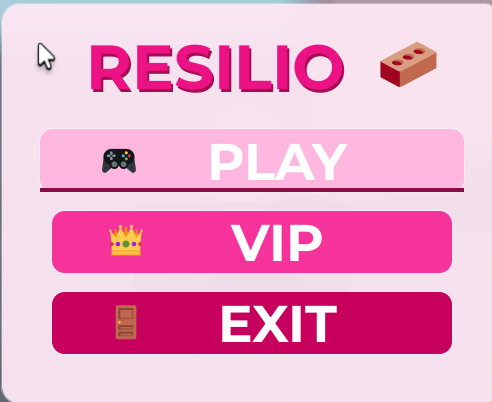
\includegraphics[width=\linewidth]{desarrollo/R1.png}
        \caption*{\textbf{Main Menu}}
    \end{minipage}
    \hfill
    \begin{minipage}[b]{0.32\textwidth}
        \centering
        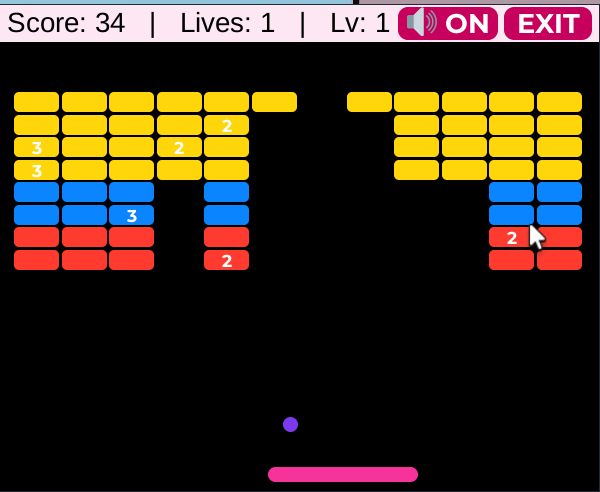
\includegraphics[width=\linewidth]{desarrollo/R12.png}
        \caption*{\textbf{Gameplay}}
    \end{minipage}
    \hfill
    \begin{minipage}[b]{0.32\textwidth}
        \centering
        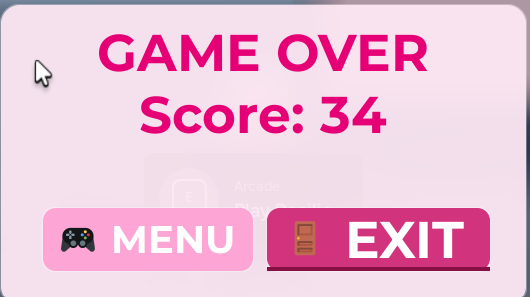
\includegraphics[width=\linewidth]{desarrollo/R13.png}
        \caption*{\textbf{Score Menu}}
    \end{minipage}
\end{figure}

\begin{figure}[H]
    \centering
    \begin{minipage}[b]{0.47\textwidth}
        \centering
        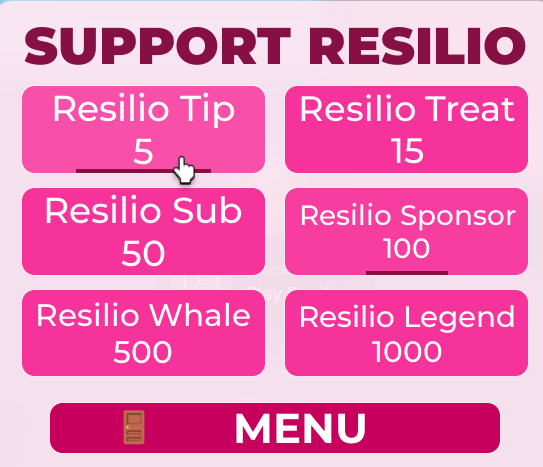
\includegraphics[width=\linewidth]{desarrollo/R14.png}
        \caption*{\textbf{VIP Menu}}
    \end{minipage}
    \hfill
    \begin{minipage}[b]{0.47\textwidth}
        \centering
        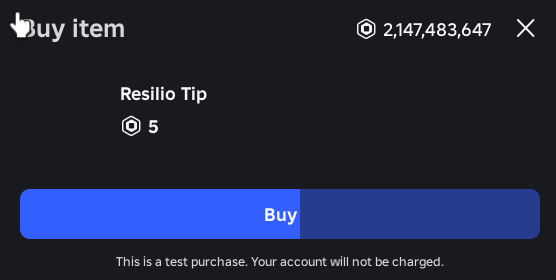
\includegraphics[width=\linewidth]{desarrollo/R15.png}
        \caption*{\textbf{Donation Interface}}
    \end{minipage}
\end{figure}

\begin{figure}[H]
    \centering
    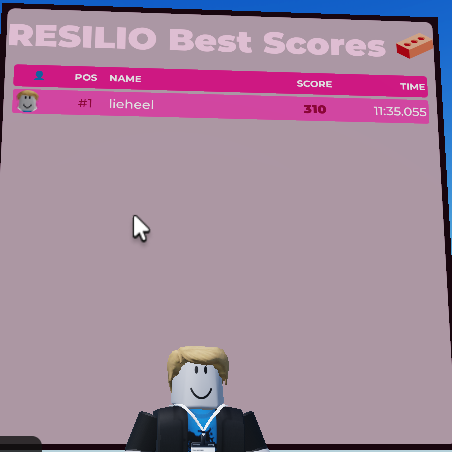
\includegraphics[width=0.6\textwidth]{desarrollo/R16.png}
    \caption*{\textbf{Global Score Table}}
\end{figure}

\clearpage

\subsection{Foxy Fruit}

Foxy Fruit is a maze based action game built inside Roblox Studio on a grid of $16 \times 12$ tiles. The hardest part to build was the bear AI. The four bears all use the same pathfinding (a breadth first search, or BFS), but each one aims at a different cell, so they end up behaving in different and hard to predict ways without having to script every single situation by hand. The game has three handmade levels and a power mode: when the player eats a blueberry, all the bears turn scared for a few seconds.

\subsubsection{Rules of Foxy Fruit}
\begin{itemize}
  \item \textbf{Main Goal:} Eat all raspberries across three levels without losing all three lives.
  \item \textbf{Controls (PC):} Arrow keys or WASD for grid based movement. Also adapted for mobile touchscreen, Xbox, and PlayStation controllers via \texttt{UniversalController}.
  \item \textbf{Collectibles:} Raspberries score 10 points each. Blueberries score 50 points and activate power mode for 4 seconds.
  \item \textbf{Power Mode:} All bears switch to frightened state and flee. Eating a frightened bear scores 200, 400, 800, or 1600 points depending on how many are eaten in one power mode activation.
  \item \textbf{Bear Behaviors:}
  \begin{itemize}
    \item \textbf{Red Bear:} Uses BFS to move directly toward the player's current cell.
    \item \textbf{Pink Bear:} Uses BFS to target a cell 4 steps ahead of the player's current direction.
    \item \textbf{Blue Bear:} Calculates a point 2 cells ahead of the player, then mirrors the red bear's position relative to that point and targets the reflected cell.
    \item \textbf{Orange Bear:} Chases the player directly (BFS) if more than 8 cells away; retreats to the bottom left corner when closer.
  \end{itemize}
  \item \textbf{Lives:} The session starts with 3 lives. Clearing a level grants 1 extra life.
  \item \textbf{End Condition:} Losing all lives ends the session. Clearing all three levels triggers a perfect game.
\end{itemize}

\textbf{Flowchart}
\begin{figure}[H]
  \centering
  \input{diagrama/foxyfruit-flow}
  \caption{Flowchart for Foxy Fruit.}
  \label{fig:foxyfruit_flow}
\end{figure}

\subsubsection{Project Structure}

Foxy Fruit follows the same four file layout as the rest of the arcade.

\begin{lstlisting}
FoxyFruit/
|-- Workspace/
|   +-- FoxyFruit/ (Folder)
|       +-- ButtonFoxyFruit        (Part, Tag="ButtonFoxyFruit")
|-- ReplicatedStorage/
|   |-- ArcadeRemotes/
|   |   +-- FoxyFruit/ (Folder)
|   |       |-- StartFoxyFruitRequest  (RemoteEvent)
|   |       |-- SubmitMove             (RemoteEvent)
|   |       |-- GameState              (RemoteEvent)
|   |       +-- ToggleAudio            (RemoteEvent)
|   +-- Modules/
|       +-- FoxyFruitModule        (ModuleScript)
|-- ServerScriptService/
|   +-- FoxyFruitServer            (Script)
+-- StarterPlayer/
    +-- StarterPlayerScripts/
        +-- FoxyFruitClient        (LocalScript)
\end{lstlisting}

\subsubsection{Time Complexity}

Each call to \texttt{update(dt)} costs $O(E \times N)$ time, where $E = 4$ is the number of bears and $N = 12 \times 16 = 192$ is the number of cells in the grid. Moving the player and eating a raspberry are $O(1)$, because the game looks the cell up directly. When a bear takes a step, it runs its BFS search from its cell to its target cell, and that search visits at most 192 cells. With 4 bears, the worst case per tick is about $4 \times 192$ steps. Sending the state to the screen goes through the grid once. Since the number of bears and the size of the grid are both fixed, all of this is really just a constant amount of work per tick, even if it looks large written out.

\subsubsection{Space Complexity}

The memory cost is $O(N)$, where $N = 192$ cells. The grid is a $12 \times 16$ table of numbers that is copied fresh each time a level loads. Every BFS search creates two small helper tables the size of the grid and throws them away as soon as it finishes. The list of bears is always 4 entries. Everything else (score, lives, the power timer, the game state) is a single value, so the memory used in a session stays within a fixed limit.

\subsubsection{Game Features and Implementation Status}

\begin{table}[H]
\centering
\begin{tabular}{|p{4cm}|p{8cm}|p{2.5cm}|}
\hline
\textbf{Feature} & \textbf{Description} & \textbf{Status} \\
\hline
Main Menu & Interface with Play, VIP, and Exit buttons. & Working \\
\hline
Menu Sounds & Audio feedback for navigation and selection. & Working \\
\hline
Gameplay Controls & Grid based movement via arrow keys or WASD. & Working \\
\hline
Mute Button & In game toggle to turn all audio on or off. & Working \\
\hline
Exit Button (Game) & Allows the player to abort the run and return to the score menu. & Working \\
\hline
Score Menu & A screen after the game showing the final score and a replay option. & Working \\
\hline
Level System & Three handmade tile maps with increasing layout complexity. Clearing a level grants 1 extra life. & Working \\
\hline
Bear AI & Four bears with distinct BFS based targeting behaviors (direct chase, ambush, flank, territorial). & Working \\
\hline
Power Mode & Eating a blueberry activates a four second frightened state on all bears with exponential score multiplier. & Working \\
\hline
Top 10 Score Table & Global leaderboard via Roblox DataStore. & Working \\
\hline
VIP Donation Menu & Opens a menu with various donation tiers. & Working \\
\hline
Optimization & $O(E \times N)$ with $E=4$ bears and $N=192$ grid cells fixed; effectively $O(1)$ per tick. & Working \\
\hline
Mobile Adaptation & Touchscreen input via \texttt{UniversalController}. & Working \\
\hline
Xbox Adaptation & Gamepad input via \texttt{UniversalController}. & Working \\
\hline
PlayStation Adaptation & DualSense and DualShock input via \texttt{UniversalController}. & Working \\
\hline
\end{tabular}
\caption{Functionalities and current status of Foxy Fruit.}
\end{table}

\subsubsection{Game Results}

\begin{figure}[H]
    \centering
    \begin{minipage}[b]{0.32\textwidth}
        \centering
        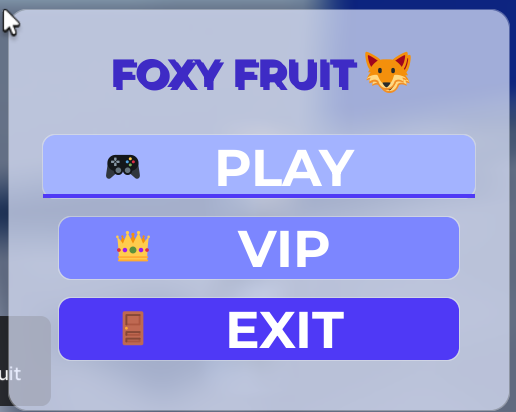
\includegraphics[width=\linewidth]{desarrollo/frutimenu.png}
        \caption*{\textbf{Main Menu}}
    \end{minipage}
    \hfill
    \begin{minipage}[b]{0.32\textwidth}
        \centering
        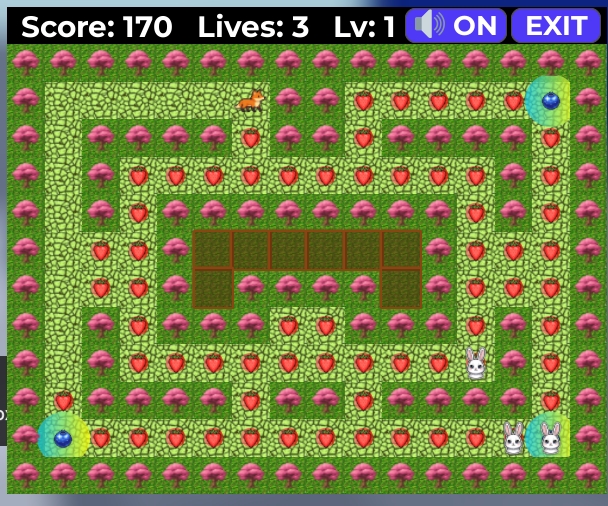
\includegraphics[width=\linewidth]{desarrollo/frutigameplay.png}
        \caption*{\textbf{Gameplay}}
    \end{minipage}
    \hfill
    \begin{minipage}[b]{0.32\textwidth}
        \centering
        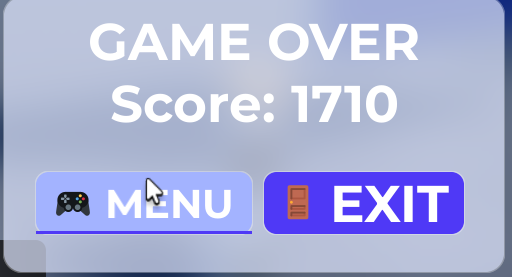
\includegraphics[width=\linewidth]{desarrollo/frutimenu2.png}
        \caption*{\textbf{Score Menu}}
    \end{minipage}
\end{figure}

\begin{figure}[H]
    \centering
    \begin{minipage}[b]{0.47\textwidth}
        \centering
        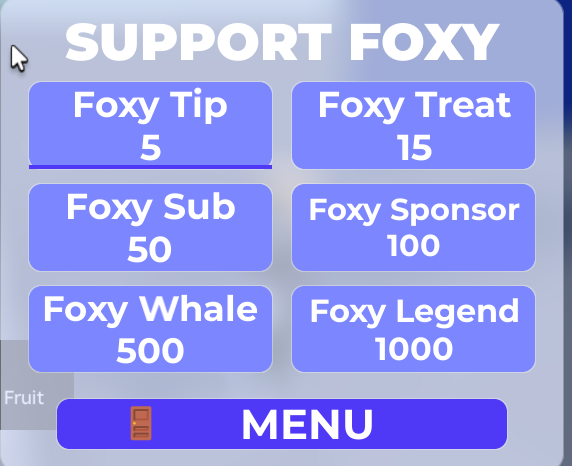
\includegraphics[width=\linewidth]{desarrollo/frutimenuvip1.png}
        \caption*{\textbf{VIP Access}}
    \end{minipage}
    \hfill
    \begin{minipage}[b]{0.47\textwidth}
        \centering
        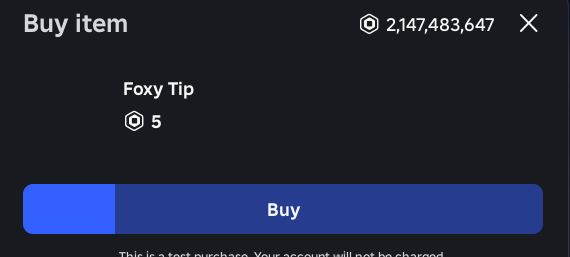
\includegraphics[width=\linewidth]{desarrollo/frutimenuvip2.png}
        \caption*{\textbf{Donation Interface}}
    \end{minipage}
\end{figure}

\begin{figure}[H]
    \centering
    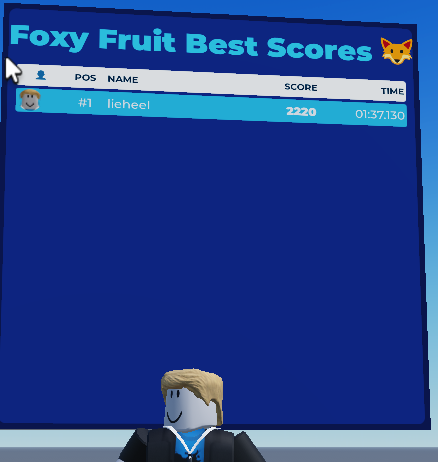
\includegraphics[width=0.6\textwidth]{desarrollo/frutiscore.png}
    \caption*{\textbf{Global Score Table}}
\end{figure}

\clearpage

\subsection{Firmament Defender}

Firmament Defender is a wave based arcade shooter built inside Roblox Studio on a $16 \times 12$ grid. The tricky part to build was the group of planes. The 30 planes move together as one block, turn around and drop a row when they reach a wall, get faster as fewer of them are left, and fire from random planes along the bottom of the group. Three waves, each one faster than the last, make the game harder over time, and once in a while a UFO crosses the top of the screen as a risky but rewarding target.

\subsubsection{Rules of Firmament Defender}
\begin{itemize}
  \item \textbf{Main Goal:} Destroy all planes across three waves before any plane descends to the ship's row.
  \item \textbf{Controls (PC):} Arrow keys or A/D to move the ship, Space to fire. Also adapted for mobile touchscreen, Xbox, and PlayStation controllers via \texttt{UniversalController}.
  \item \textbf{Plane Types:} Type C (top row, 300 pts), Type B (middle two rows, 200 pts), Type A (bottom two rows, 100 pts). Destroying one of the last 5 surviving planes adds a bonus of 500 points.
  \item \textbf{Swarm Movement:} Planes march horizontally as a single unit. When the leftmost or rightmost plane reaches a wall, the entire group drops one row and reverses direction. The base step interval is 1.20\,s.
  \item \textbf{Low Count Boost:} When 5 or fewer planes remain, their step interval drops to 65\% of its current value, down to a minimum of 0.30\,s.
  \item \textbf{Enemy Fire:} Every 0.40 to 1.40\,s (scaled by plane count), up to 3 random bottom row planes fire downward simultaneously.
  \item \textbf{Shields:} Four shield positions, each 2 cells wide and 3 HP. Both player and enemy bullets damage shields.
  \item \textbf{UFO:} Spawns every 8 to 16\,s and crosses row 1 horizontally. Shooting it scores 1000 points and grants 1 extra life.
  \item \textbf{Waves:} Three waves total. Clearing a wave grants 1 extra life and reduces the plane step interval by 10\%.
  \item \textbf{End Condition:} Losing all 4 lives or any plane reaching the ship's row ends the session. Clearing all three waves is a perfect game.
\end{itemize}

\textbf{Flowchart}
\begin{figure}[H]
  \centering
  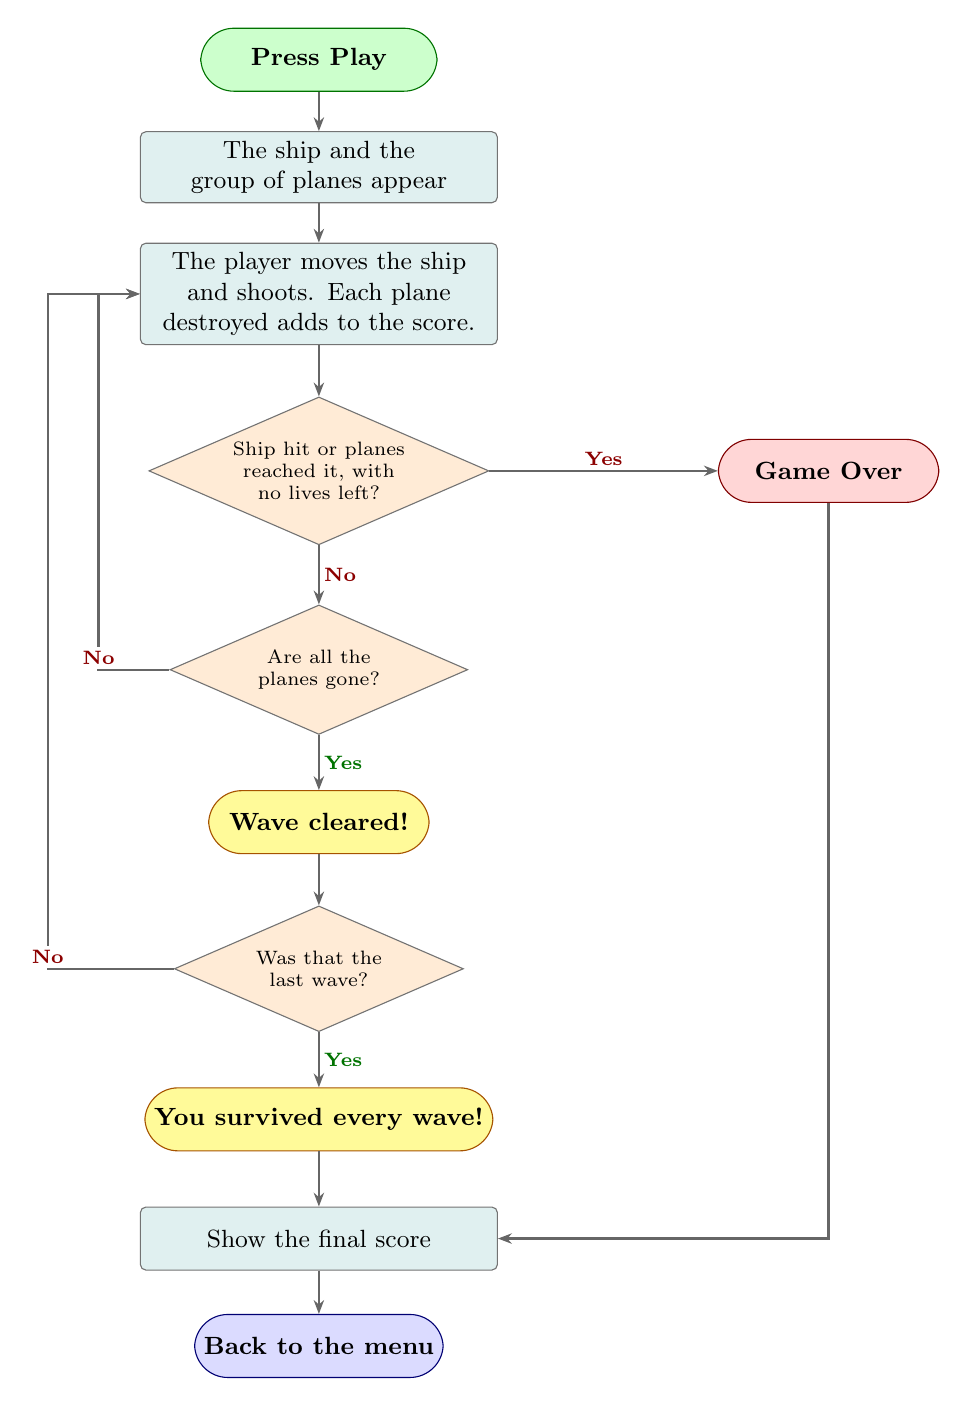
\begin{tikzpicture}[
  font=\small,
  >={Stealth[length=5pt]},
  start/.style={rectangle, rounded corners=12pt, draw=green!45!black, fill=green!20,
                minimum width=3cm, minimum height=0.8cm, align=center, font=\small\bfseries},
  menu/.style={rectangle, rounded corners=12pt, draw=blue!45!black, fill=blue!14,
               minimum width=3cm, minimum height=0.8cm, align=center, font=\small\bfseries},
  over/.style={rectangle, rounded corners=12pt, draw=red!50!black, fill=red!16,
               minimum width=2.8cm, minimum height=0.8cm, align=center, font=\small\bfseries},
  win/.style={rectangle, rounded corners=12pt, draw=orange!65!black, fill=yellow!40,
              minimum width=2.8cm, minimum height=0.8cm, align=center, font=\small\bfseries},
  act/.style={rectangle, draw=black!55, fill=teal!12, rounded corners=2pt,
              text width=4.3cm, minimum height=0.8cm, align=center},
  dec/.style={diamond, draw=black!55, fill=orange!16, aspect=2.3,
              align=center, inner sep=1pt, text width=2.4cm, font=\scriptsize},
  link/.style={->, thick, draw=black!60},
  yeslbl/.style={font=\scriptsize\bfseries, color=green!45!black, fill=white, inner sep=1.5pt},
  nolbl/.style={font=\scriptsize\bfseries, color=red!55!black, fill=white, inner sep=1.5pt},
]

\node[start] (s) {Press Play};
\node[act, below=0.5cm of s]      (init)   {The ship and the group of planes appear};
\node[act, below=0.5cm of init]   (play)   {The player moves the ship and shoots. Each plane destroyed adds to the score.};
\node[dec, below=0.65cm of play]  (lost)   {Ship hit or planes reached it, with no lives left?};
\node[dec, below=0.75cm of lost]  (clear)  {Are all the planes gone?};
\node[win, below=0.7cm of clear]  (cleared){Wave cleared!};
\node[dec, below=0.65cm of cleared](last)  {Was that the last wave?};
\node[win, below=0.7cm of last]   (finish) {You survived every wave!};
\node[act, below=0.7cm of finish] (score)  {Show the final score};
\node[menu, below=0.55cm of score](back)   {Back to the menu};

\node[over, right=2.9cm of lost]  (go)     {Game Over};

\draw[link] (s) -- (init);
\draw[link] (init) -- (play);
\draw[link] (play) -- (lost);
\draw[link] (lost) -- node[nolbl, right]{No} (clear);
\draw[link] (lost.east) -- node[nolbl, above]{Yes} (go.west);
\draw[link] (clear) -- node[yeslbl, right]{Yes} (cleared);
\draw[link] (cleared) -- (last);
\draw[link] (last) -- node[yeslbl, right]{Yes} (finish);
\draw[link] (finish) -- (score);
\draw[link] (score) -- (back);
\draw[link] (go) |- (score.east);
\draw[link] (clear.west) -- ++(-0.9,0) node[nolbl, above]{No} |- (play.west);
\draw[link] (last.west) -- ++(-1.6,0) node[nolbl, above]{No} |- (play.west);

\end{tikzpicture}

  \caption{Flowchart for Firmament Defender.}
  \label{fig:firmamentdefender_flow}
\end{figure}

\subsubsection{Project Structure}

Firmament Defender follows the same four file layout as the rest of the arcade.

\begin{lstlisting}
FirmamentDefender/
|-- Workspace/
|   +-- FirmamentDefender/ (Folder)
|       +-- ButtonFirmamentDefender  (Part, Tag="ButtonFirmamentDefender")
|-- ReplicatedStorage/
|   |-- ArcadeRemotes/
|   |   +-- FirmamentDefender/ (Folder)
|   |       |-- StartFirmamentDefenderRequest  (RemoteEvent)
|   |       |-- SubmitMove                     (RemoteEvent)
|   |       |-- GameState                      (RemoteEvent)
|   |       +-- ToggleAudio                    (RemoteEvent)
|   +-- Modules/
|       +-- FirmamentDefenderModule  (ModuleScript)
|-- ServerScriptService/
|   +-- FirmamentDefenderServer      (Script)
+-- StarterPlayer/
    +-- StarterPlayerScripts/
        +-- FirmamentDefenderClient  (LocalScript)
\end{lstlisting}

\subsubsection{Time Complexity}

Each call to \texttt{update(dt)} costs $O(N)$ time, where $N$ is the number of planes, which is never more than 30. Moving the ship is $O(1)$. Moving the whole group of planes and checking them against the shields goes through all the planes, which gives the $O(N)$. Choosing which planes shoot also goes through the list and picks up to 3, again $O(N)$. Checking the player's bullet against the planes is $O(N)$ too, and there is never more than one player bullet at a time. The UFO is $O(1)$. Because the number of planes only goes down as the player destroys them, the game actually gets lighter as each wave goes on. Sending the state to the screen copies the planes and shields once.

\subsubsection{Space Complexity}

The memory cost is $O(N)$, where $N$ is at most 30 planes at the start of a wave. The game keeps the position and type of each plane, the 8 shield pieces (4 shields, 2 cells each), and the bullets. There is only ever one player bullet at a time, and the enemy bullets can never be more than the 12 rows of the grid. Everything else (the ship position, the wave number, the timers) is a single value, so the memory used in a session stays within a fixed limit.

\subsubsection{Game Features and Implementation Status}

\begin{table}[H]
\centering
\begin{tabular}{|p{4cm}|p{8cm}|p{2.5cm}|}
\hline
\textbf{Feature} & \textbf{Description} & \textbf{Status} \\
\hline
Main Menu & Interface with Play, VIP, and Exit buttons. & Working \\
\hline
Menu Sounds & Audio feedback for navigation and selection. & Working \\
\hline
Gameplay Controls & Ship movement (left/right) and continuous fire. & Working \\
\hline
Mute Button & In game toggle to turn all audio on or off. & Working \\
\hline
Exit Button (Game) & Allows the player to abort the run and return to the score menu. & Working \\
\hline
Score Menu & A screen after the game showing the final score and a replay option. & Working \\
\hline
Wave System & Three waves of increasing speed (step interval $\times 0.9$ per wave). Clearing a wave grants 1 extra life. & Working \\
\hline
Plane Swarm Logic & 30 planes march as a group, drop and reverse at walls, and accelerate when 5 or fewer remain. & Working \\
\hline
Plane Type Scoring & Type A = 100 pts, Type B = 200 pts, Type C = 300 pts. Last 5 alive grant +500 bonus each. & Working \\
\hline
Destructible Shields & Four shield positions, 2 cells wide, 3 HP each. Damaged by both player and enemy bullets. & Working \\
\hline
UFO & Spawns every 8 to 16\,s, crosses row 1, worth 1000 points and 1 extra life on hit. & Working \\
\hline
Top 10 Score Table & Global leaderboard via Roblox DataStore. & Working \\
\hline
VIP Donation Menu & Opens a menu with various donation tiers. & Working \\
\hline
Optimization & $O(N)$ per tick with $N \leq 30$ decreasing monotonically; player bullet capped at 1. & Working \\
\hline
Mobile Adaptation & Touchscreen input via \texttt{UniversalController}. & Working \\
\hline
Xbox Adaptation & Gamepad input via \texttt{UniversalController}. & Working \\
\hline
PlayStation Adaptation & DualSense and DualShock input via \texttt{UniversalController}. & Working \\
\hline
\end{tabular}
\caption{Functionalities and current status of Firmament Defender.}
\end{table}

\subsubsection{Game Results}

\begin{figure}[H]
    \centering
    \begin{minipage}[b]{0.32\textwidth}
        \centering
        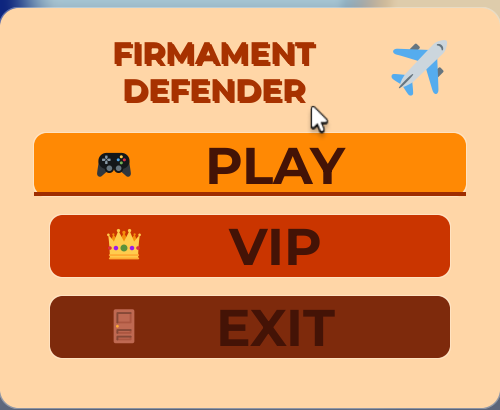
\includegraphics[width=\linewidth]{desarrollo/fir1.png}
        \caption*{\textbf{Main Menu}}
    \end{minipage}
    \hfill
    \begin{minipage}[b]{0.32\textwidth}
        \centering
        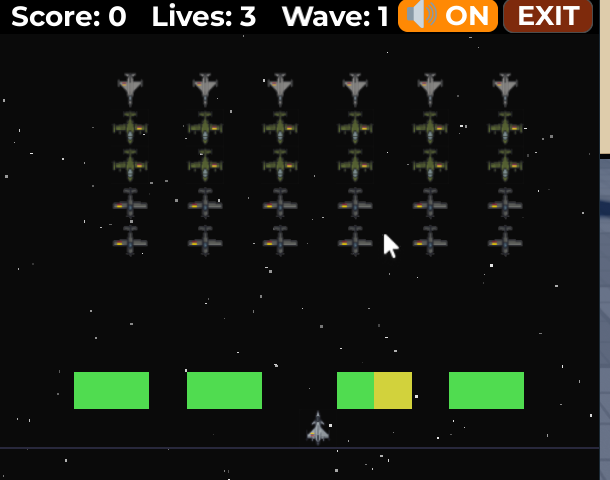
\includegraphics[width=\linewidth]{desarrollo/fir0.png}
        \caption*{\textbf{Gameplay}}
    \end{minipage}
    \hfill
    \begin{minipage}[b]{0.32\textwidth}
        \centering
        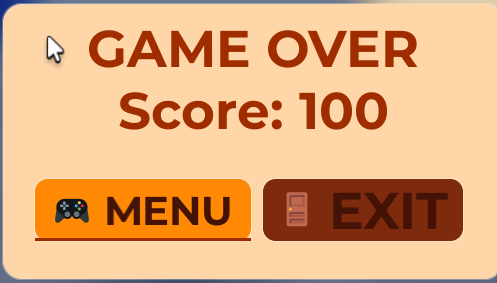
\includegraphics[width=\linewidth]{desarrollo/fir3.png}
        \caption*{\textbf{Score Menu}}
    \end{minipage}
\end{figure}

\begin{figure}[H]
    \centering
    \begin{minipage}[b]{0.47\textwidth}
        \centering
        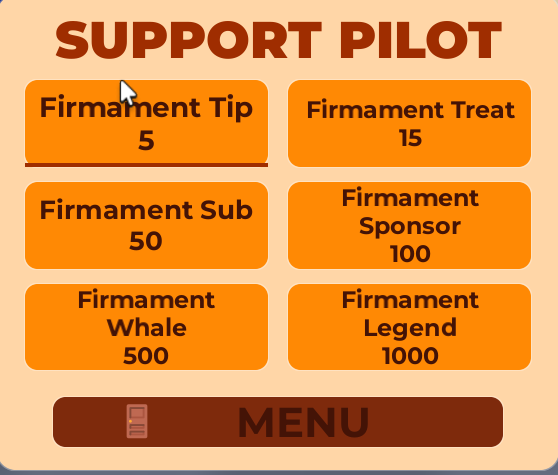
\includegraphics[width=\linewidth]{desarrollo/fir4.png}
        \caption*{\textbf{VIP Menu}}
    \end{minipage}
    \hfill
    \begin{minipage}[b]{0.47\textwidth}
        \centering
        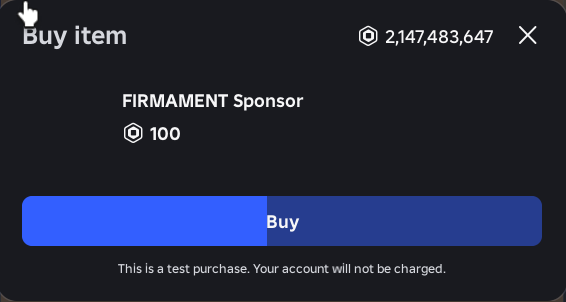
\includegraphics[width=\linewidth]{desarrollo/fir5.png}
        \caption*{\textbf{Donation Interface}}
    \end{minipage}
\end{figure}

\begin{figure}[H]
    \centering
    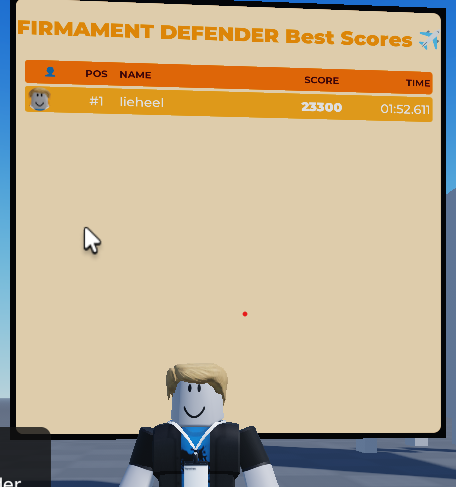
\includegraphics[width=0.6\textwidth]{desarrollo/fir6.png}
    \caption*{\textbf{Global Score Table}}
\end{figure}

\clearpage

\subsection{Firmament Siege}

Firmament Siege is a survival shooter with free movement, built inside Roblox Studio on a $16 \times 12$ open space. It had three main challenges. The first was the ship physics: the ship keeps drifting after the player stops pushing, and slows down little by little instead of stopping at once. The second was the screen wrapping: when the ship, a drone, or a bullet leaves one edge, it comes back from the opposite edge. The third was the aiming: the player can shoot in any direction, no matter which way the ship is moving. The game never really ends. Drones are destroyed and new ones appear, so there are always between 4 and 7 of them on screen.

\subsubsection{Rules of Firmament Siege}
\begin{itemize}
  \item \textbf{Main Goal:} Survive as long as possible and accumulate the highest score by destroying drones.
  \item \textbf{Controls (PC):} WASD or arrow keys to thrust the ship in eight directions, mouse to aim, click or Space to fire, H for hyperspace. Also adapted for mobile touchscreen, Xbox, and PlayStation controllers via \texttt{UniversalController}.
  \item \textbf{Ship Physics:} The ship accelerates at 35 cells/s\textsuperscript{2} up to a maximum of 10 cells/s. Releasing the thrust keys applies exponential damping ($0.82^{60\Delta t}$ per frame) rather than an instant stop.
  \item \textbf{Screen Wrapping:} The ship, all drones, and all bullets wrap toroidally: exiting one edge of the grid immediately reappears on the opposite edge.
  \item \textbf{Bullets:} Fire rate is capped at one bullet every 80\,ms. Each bullet travels at 23 cells/s and disappears after 0.8\,s (maximum range 18.4 cells).
  \item \textbf{Drone Types:} Type A (smallest, 1.4 to 2.2 cells/s, 150 pts), Type B (medium, 1.6 to 2.4 cells/s, 100 pts), Type C (largest, 1.8 to 2.6 cells/s, 50 pts). All drones steer directly toward the ship using toroidal vector math.
  \item \textbf{Dynamic Composition:} Every 3.2\,s the game picks a new target total (4 to 7 drones) and spawns the missing drones outside a safety radius of 7 cells around the ship. The mix of drone types follows a fixed ratio for each total count.
  \item \textbf{Hyperspace:} Teleports the ship to a random position and grants a brief 0.6\,s invulnerability extension.
  \item \textbf{Lives:} Three lives. After each death the ship respawns at the grid center with 1.1\,s of invulnerability and nearby drones cleared.
  \item \textbf{End Condition:} Losing all three lives ends the session. The game has no win state: it runs until the player dies.
\end{itemize}

\textbf{Flowchart}
\begin{figure}[H]
  \centering
  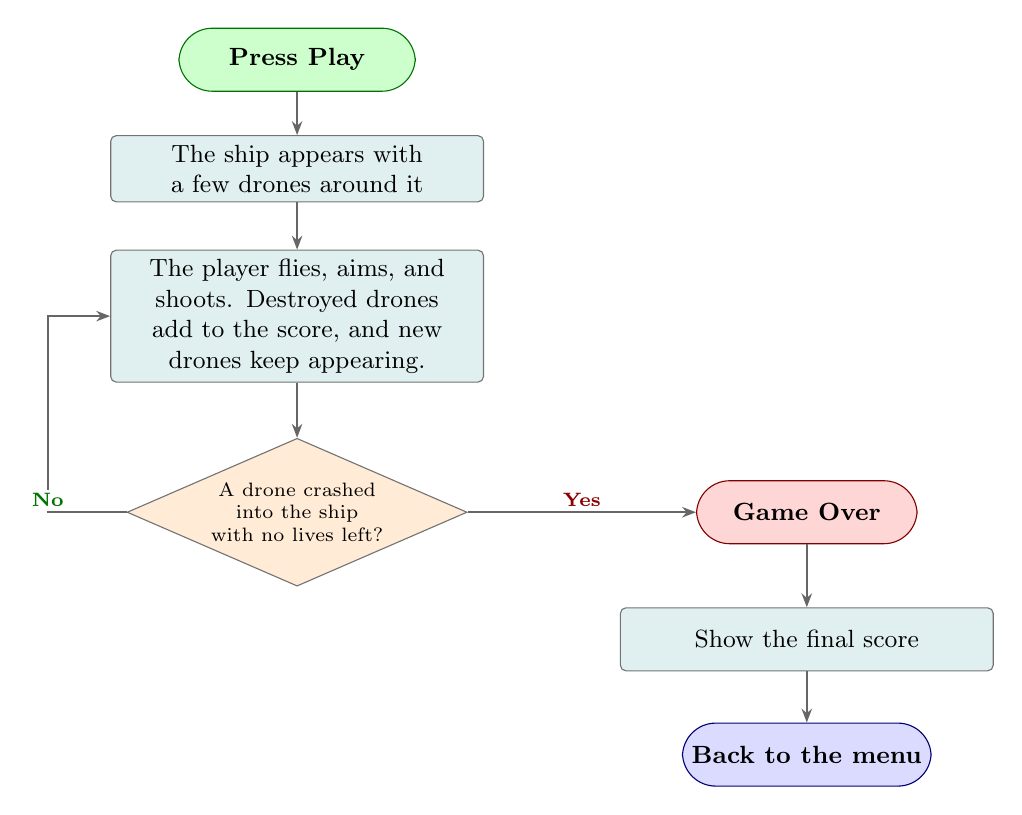
\begin{tikzpicture}[
  font=\small,
  >={Stealth[length=5pt]},
  start/.style={rectangle, rounded corners=12pt, draw=green!45!black, fill=green!20,
                minimum width=3cm, minimum height=0.8cm, align=center, font=\small\bfseries},
  menu/.style={rectangle, rounded corners=12pt, draw=blue!45!black, fill=blue!14,
               minimum width=3cm, minimum height=0.8cm, align=center, font=\small\bfseries},
  over/.style={rectangle, rounded corners=12pt, draw=red!50!black, fill=red!16,
               minimum width=2.8cm, minimum height=0.8cm, align=center, font=\small\bfseries},
  act/.style={rectangle, draw=black!55, fill=teal!12, rounded corners=2pt,
              text width=4.5cm, minimum height=0.8cm, align=center},
  dec/.style={diamond, draw=black!55, fill=orange!16, aspect=2.3,
              align=center, inner sep=1pt, text width=2.4cm, font=\scriptsize},
  link/.style={->, thick, draw=black!60},
  yeslbl/.style={font=\scriptsize\bfseries, color=green!45!black, fill=white, inner sep=1.5pt},
  nolbl/.style={font=\scriptsize\bfseries, color=red!55!black, fill=white, inner sep=1.5pt},
]

\node[start] (s) {Press Play};
\node[act, below=0.55cm of s]   (init) {The ship appears with a few drones around it};
\node[act, below=0.6cm of init] (play) {The player flies, aims, and shoots. Destroyed drones add to the score, and new drones keep appearing.};
\node[dec, below=0.7cm of play] (crash){A drone crashed into the ship with no lives left?};

\node[over, right=2.9cm of crash]  (go)   {Game Over};
\node[act, below=0.8cm of go]      (score){Show the final score};
\node[menu, below=0.65cm of score] (back) {Back to the menu};

\draw[link] (s) -- (init);
\draw[link] (init) -- (play);
\draw[link] (play) -- (crash);
\draw[link] (crash.east) -- node[nolbl, above]{Yes} (go.west);
\draw[link] (crash.west) -- ++(-1.0,0) node[yeslbl, above]{No} |- (play.west);
\draw[link] (go) -- (score);
\draw[link] (score) -- (back);

\end{tikzpicture}

  \caption{Flowchart for Firmament Siege.}
  \label{fig:firmamentsiege_flow}
\end{figure}

\subsubsection{Project Structure}

Firmament Siege follows the same four file layout as the rest of the arcade.

\begin{lstlisting}
FirmamentSiege/
|-- Workspace/
|   +-- FirmamentSiege/ (Folder)
|       +-- ButtonFirmamentSiege       (Part, Tag="ButtonFirmamentSiege")
|-- ReplicatedStorage/
|   |-- ArcadeRemotes/
|   |   +-- FirmamentSiege/ (Folder)
|   |       |-- StartFirmamentSiegeRequest  (RemoteEvent)
|   |       |-- SubmitMove                  (RemoteEvent)
|   |       |-- GameState                   (RemoteEvent)
|   |       +-- ToggleAudio                 (RemoteEvent)
|   +-- Modules/
|       +-- FirmamentSiegeModule       (ModuleScript)
|-- ServerScriptService/
|   +-- FirmamentSiegeServer           (Script)
+-- StarterPlayer/
    +-- StarterPlayerScripts/
        +-- FirmamentSiegeClient       (LocalScript)
\end{lstlisting}

\subsubsection{Time Complexity}

Each call to \texttt{update(dt)} costs $O(N \times M)$ time, where $N$ is the number of drones (never more than 7) and $M$ is the number of bullets on screen. Moving the ship is $O(1)$. Moving the bullets is $O(M)$, and steering the drones toward the ship is $O(N)$. The most expensive step is checking every bullet against every drone, which is $O(N \times M)$. The number of bullets is limited too: the ship can only fire one bullet every 80 milliseconds and each bullet lasts 0.8 seconds, so there are never more than about 10 bullets at once. With 7 drones and 10 bullets, the worst case is around 70 checks, which is a small fixed number. Sending the state to the screen copies the drones and bullets once.

\subsubsection{Space Complexity}

The memory cost is $O(N + M)$, with at most 7 drones and 10 bullets, both fixed numbers. Each drone keeps its position, speed, type, and rotation, and each bullet keeps its position, speed, and how much time it has left. Everything else (the ship's position and speed, the aim angle, the timers, the score, the lives) is a single value. Because of this, the memory used stays within a fixed limit no matter how long the game runs.

\subsubsection{Game Features and Implementation Status}

\begin{table}[H]
\centering
\begin{tabular}{|p{4cm}|p{8cm}|p{2.5cm}|}
\hline
\textbf{Feature} & \textbf{Description} & \textbf{Status} \\
\hline
Main Menu & Interface with Play, VIP, and Exit buttons. & Working \\
\hline
Menu Sounds & Audio feedback for navigation and selection. & Working \\
\hline
Gameplay Controls & eight direction thrust, free aim shooting, and hyperspace teleport. & Working \\
\hline
Mute Button & In game toggle to turn all audio on or off. & Working \\
\hline
Exit Button (Game) & Allows the player to abort the run and return to the score menu. & Working \\
\hline
Score Menu & A screen after the game showing the final score and a replay option. & Working \\
\hline
Physics Engine & Inertia based movement with exponential damping and toroidal screen wrapping for all entities. & Working \\
\hline
Drone AI & Three drone types steer toward the ship via toroidal vector math at different speeds (1.4 to 2.6 cells/s). & Working \\
\hline
Dynamic Composition & Target drone count (4 to 7) chosen again every 3.2\,s; missing drones spawn outside a safety radius of 7 cells. & Working \\
\hline
Hyperspace & Teleports the ship to a random safe position with a brief invulnerability extension. & Working \\
\hline
Top 10 Score Table & Global leaderboard via Roblox DataStore. & Working \\
\hline
VIP Donation Menu & Opens a menu with various donation tiers. & Working \\
\hline
Optimization & $O(N \times M)$ per tick with $N \leq 7$ drones and $M \leq 10$ bullets; effectively $O(1)$. & Working \\
\hline
Mobile Adaptation & Touchscreen input via \texttt{UniversalController}. & Working \\
\hline
Xbox Adaptation & Gamepad input via \texttt{UniversalController}. & Working \\
\hline
PlayStation Adaptation & DualSense and DualShock input via \texttt{UniversalController}. & Working \\
\hline
\end{tabular}
\caption{Functionalities and current status of Firmament Siege.}
\end{table}

\subsubsection{Game Results}

\begin{figure}[H]
    \centering
    \begin{minipage}[b]{0.32\textwidth}
        \centering
        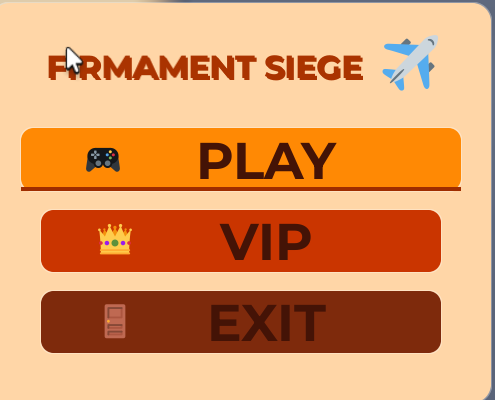
\includegraphics[width=\linewidth]{desarrollo/fd1.png}
        \caption*{\textbf{Main Menu}}
    \end{minipage}
    \hfill
    \begin{minipage}[b]{0.32\textwidth}
        \centering
        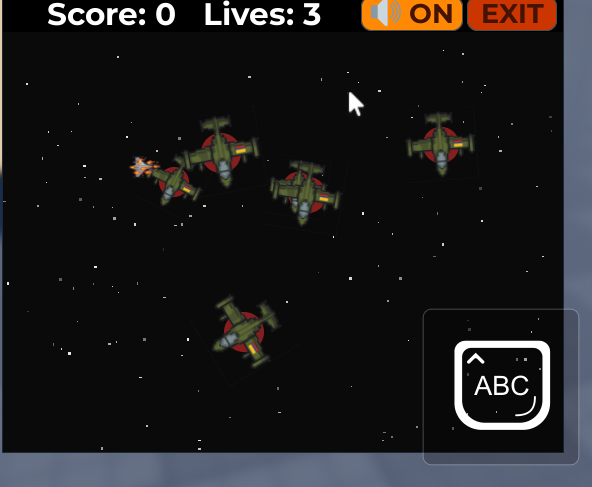
\includegraphics[width=\linewidth]{desarrollo/fd2.png}
        \caption*{\textbf{Gameplay}}
    \end{minipage}
    \hfill
    \begin{minipage}[b]{0.32\textwidth}
        \centering
        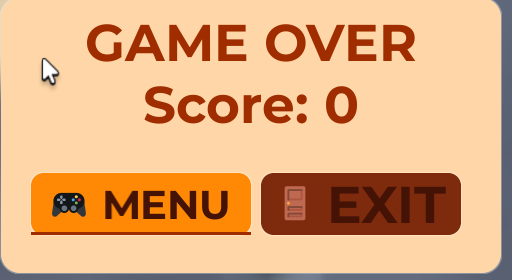
\includegraphics[width=\linewidth]{desarrollo/fd3.png}
        \caption*{\textbf{Score Menu}}
    \end{minipage}
\end{figure}

\begin{figure}[H]
    \centering
    \begin{minipage}[b]{0.47\textwidth}
        \centering
        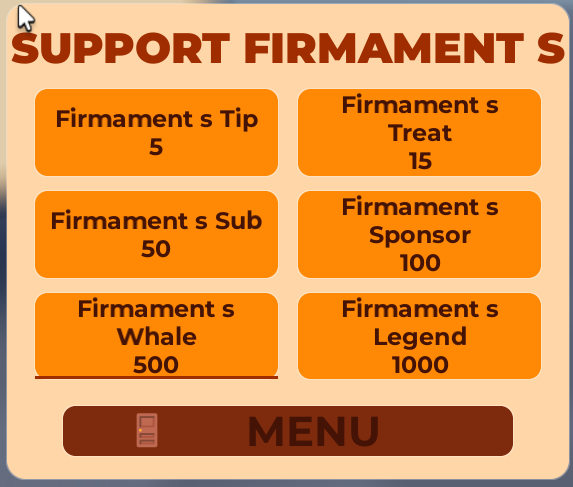
\includegraphics[width=\linewidth]{desarrollo/fd4.png}
        \caption*{\textbf{VIP Menu}}
    \end{minipage}
    \hfill
    \begin{minipage}[b]{0.47\textwidth}
        \centering
        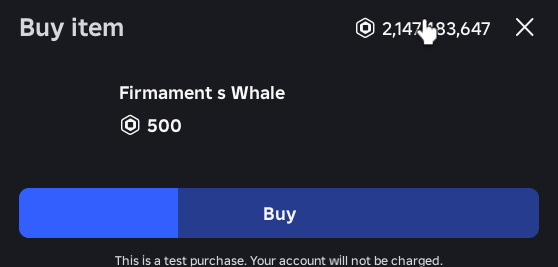
\includegraphics[width=\linewidth]{desarrollo/fd5.png}
        \caption*{\textbf{Donation Interface}}
    \end{minipage}
\end{figure}

\begin{figure}[H]
    \centering
    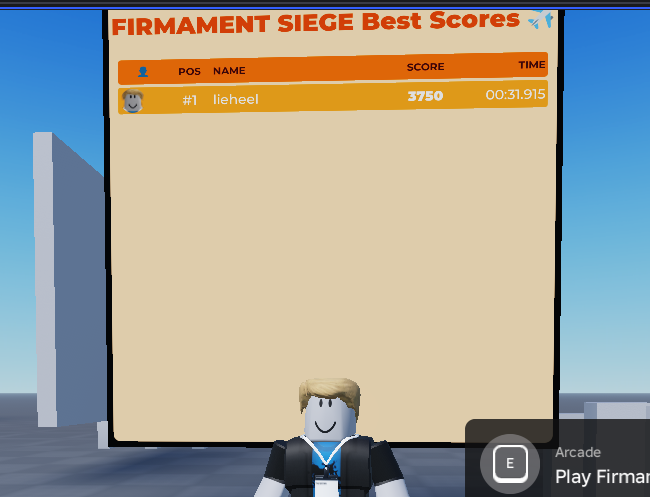
\includegraphics[width=0.6\textwidth]{desarrollo/fd6.png}
    \caption*{\textbf{Global Score Table}}
\end{figure}

\clearpage

\subsection{Juice Cutter}

Juice Cutter is a swipe based arcade game built inside Roblox Studio on a canvas of $380 \times 360$ pixels. Fruits fly up into the air and fall back down, and the player cuts them by drawing lines across the screen with a swipe. What makes it different is the recipe system: each of the five levels asks for certain fruits (for example, 15 lemons, or 12 cucumbers, 12 kiwis, and 12 green apples). Cutting the wrong fruit costs a life and takes away points, so paying attention to what is in the air matters as much as fast reactions.

\subsubsection{Rules of Juice Cutter}
\begin{itemize}
  \item \textbf{Main Goal:} Complete the recipe for each of the five levels by cutting the required fruits before running out of lives.
  \item \textbf{Controls (PC):} Click and drag the mouse to draw a cut line. Also adapted for mobile touchscreen, Xbox, and PlayStation controllers via \texttt{UniversalController}.
  \item \textbf{Cut Detection:} A cut is registered when the swipe line segment passes within 40 pixels of a fruit center (point to segment distance test).
  \item \textbf{Good Fruits:} Cutting a target fruit scores points and counts toward the recipe goal.
  \item \textbf{Bad Fruits:} Cutting a wrong fruit deducts the same number of points and removes one life.
  \item \textbf{Physics:} Fruits launch from the bottom of the canvas at 520 to 850\,px/s (varies by level) with a random horizontal velocity of $\pm220$\,px/s. Gravity pulls them down at 950\,px/s\textsuperscript{2}. They bounce off side walls and disappear when they fall below the canvas.
  \item \textbf{Levels:}
  \begin{itemize}
    \item Level 1 (Lemonade): 20 lemons, 50 pts each, 65\% chance of a good fruit.
    \item Level 2 (StrawBanana): 15 strawberries and 15 bananas, 100 pts each, 60\% chance of a good fruit.
    \item Level 3 (Tropical): 12 pineapples, 12 coconuts, and 12 cherries, 150 pts each, 55\%.
    \item Level 4 (Green Detox): 12 cucumbers, 12 green apples, and 12 kiwis, 200 pts each, 48\%.
    \item Level 5 (Pure Red Juice): 15 grapes, 15 red apples, and 15 oranges, 250 pts each, 42\%.
  \end{itemize}
  \item \textbf{Lives:} Level 1 starts with 5 lives. Completing a level carries lives over with a +1 bonus.
  \item \textbf{Weighted Spawning:} In split goal levels, the spawner biases toward fruit kinds that still need to be cut, reducing blind luck situations near the end of a level.
\end{itemize}

\textbf{Flowchart}
\begin{figure}[H]
  \centering
  \input{diagrama/juicecutter-flow}
  \caption{Flowchart for Juice Cutter.}
  \label{fig:juicecutter_flow}
\end{figure}

\subsubsection{Project Structure}

Juice Cutter follows the same four file layout as the rest of the arcade.

\begin{lstlisting}
JuiceCutter/
|-- Workspace/
|   +-- JuiceCutter/ (Folder)
|       +-- ButtonJuiceCutter        (Part, Tag="ButtonJuiceCutter")
|-- ReplicatedStorage/
|   |-- ArcadeRemotes/
|   |   +-- JuiceCutter/ (Folder)
|   |       |-- StartJuiceCutterRequest  (RemoteEvent)
|   |       |-- SubmitMove               (RemoteEvent)
|   |       |-- GameState                (RemoteEvent)
|   |       +-- ToggleAudio              (RemoteEvent)
|   +-- Modules/
|       +-- JuiceCutterModule        (ModuleScript)
|-- ServerScriptService/
|   +-- JuiceCutterServer            (Script)
+-- StarterPlayer/
    +-- StarterPlayerScripts/
        +-- JuiceCutterClient        (LocalScript)
\end{lstlisting}

\subsubsection{Time Complexity}

Each call to \texttt{step(dt)} costs $O(F)$ time, where $F$ is the number of fruits in the air. Deciding whether to spawn a new fruit is $O(1)$. Updating the fruits goes through all of them to apply gravity, move them, bounce them off the walls, and remove the ones that have fallen off the screen, which gives the $O(F)$. Checking a swipe also goes through the fruits once to see which ones it cut. Sending the state to the screen copies the fruit list once. There are never many fruits at the same time: even at the fastest level, a fruit is only on screen for about half a second, so only a few are in the air at any moment. In practice the count stays well under 10, so the real cost is basically constant.

\subsubsection{Space Complexity}

The memory cost is $O(F)$, where $F$ is the small number of fruits in the air. Each fruit keeps its position, speed, rotation, kind, images, and whether it has been cut. The game also keeps a small counter for each kind of fruit the level needs, and a level never asks for more than 3 kinds. Everything else (score, lives, the current level, the spawn timer, the goal counters) is a single value, so the memory used in a session stays within a fixed limit.

\subsubsection{Game Features and Implementation Status}

\begin{table}[H]
\centering
\begin{tabular}{|p{4cm}|p{8cm}|p{2.5cm}|}
\hline
\textbf{Feature} & \textbf{Description} & \textbf{Status} \\
\hline
Main Menu & Interface with Play, VIP, and Exit buttons. & Working \\
\hline
Menu Sounds & Audio feedback for navigation and selection. & Working \\
\hline
Gameplay Controls & Click and drag swipe to cut fruits flying across the canvas. & Working \\
\hline
Mute Button & In game toggle to turn all audio on or off. & Working \\
\hline
Exit Button (Game) & Allows the player to abort the run and return to the score menu. & Working \\
\hline
Score Menu & A screen after the game showing the final score and a replay option. & Working \\
\hline
Level System & Five levels with unique recipes and increasing difficulty. Lives carry over with a +1 bonus per level cleared. & Working \\
\hline
Recipe System & Per level goals tracked per fruit kind. Weighted spawner biases toward still needed kinds in split goal levels. & Working \\
\hline
Physics Engine & Gravity (950\,px/s\textsuperscript{2}), side wall bounce, random spin, and cut linger animation (1.2\,s) per fruit. & Working \\
\hline
Cut Detection & Point to segment distance test against a 40\,px radius per fruit; fires once per swipe event. & Working \\
\hline
Top 10 Score Table & Global leaderboard via Roblox DataStore. & Working \\
\hline
VIP Donation Menu & Opens a menu with various donation tiers. & Working \\
\hline
Optimization & $O(F)$ per tick with $F \leq 10$ active fruits; effectively $O(1)$. & Working \\
\hline
Mobile Adaptation & Touchscreen swipe input via \texttt{UniversalController}. & Working \\
\hline
Xbox Adaptation & Gamepad input via \texttt{UniversalController}. & Working \\
\hline
PlayStation Adaptation & DualSense and DualShock input via \texttt{UniversalController}. & Working \\
\hline
\end{tabular}
\caption{Functionalities and current status of Juice Cutter.}
\end{table}

\subsubsection{Game Results}

\begin{figure}[H]
    \centering
    \begin{minipage}[b]{0.32\textwidth}
        \centering
        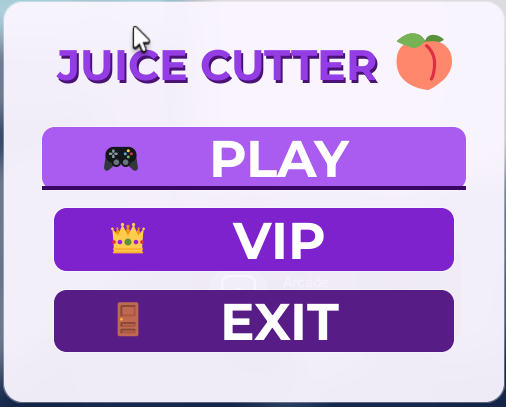
\includegraphics[width=\linewidth]{desarrollo/j1.png}
        \caption*{\textbf{Main Menu}}
    \end{minipage}
    \hfill
    \begin{minipage}[b]{0.32\textwidth}
        \centering
        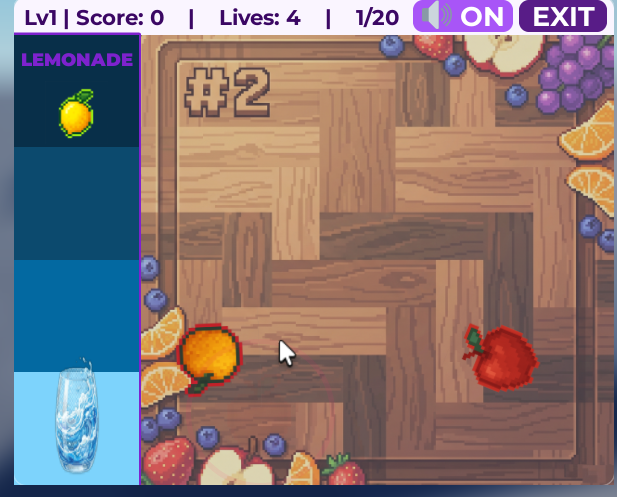
\includegraphics[width=\linewidth]{desarrollo/j2.png}
        \caption*{\textbf{Gameplay}}
    \end{minipage}
    \hfill
    \begin{minipage}[b]{0.32\textwidth}
        \centering
        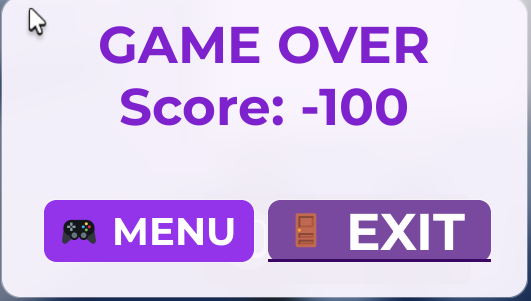
\includegraphics[width=\linewidth]{desarrollo/j3.png}
        \caption*{\textbf{Score Menu}}
    \end{minipage}
\end{figure}

\begin{figure}[H]
    \centering
    \begin{minipage}[b]{0.47\textwidth}
        \centering
        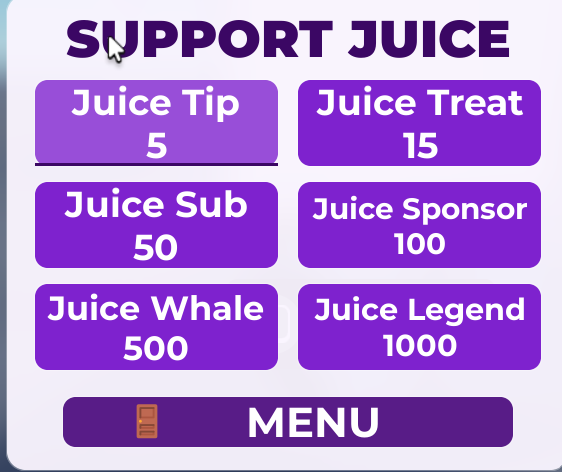
\includegraphics[width=\linewidth]{desarrollo/j4.png}
        \caption*{\textbf{VIP Menu}}
    \end{minipage}
    \hfill
    \begin{minipage}[b]{0.47\textwidth}
        \centering
        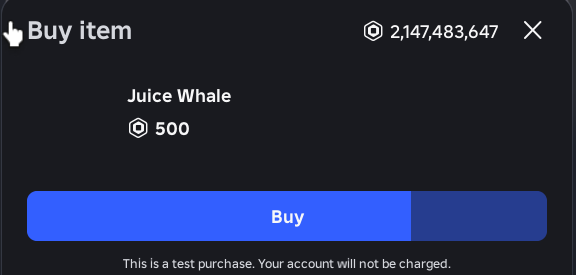
\includegraphics[width=\linewidth]{desarrollo/j5.png}
        \caption*{\textbf{Donation Interface}}
    \end{minipage}
\end{figure}

\begin{figure}[H]
    \centering
    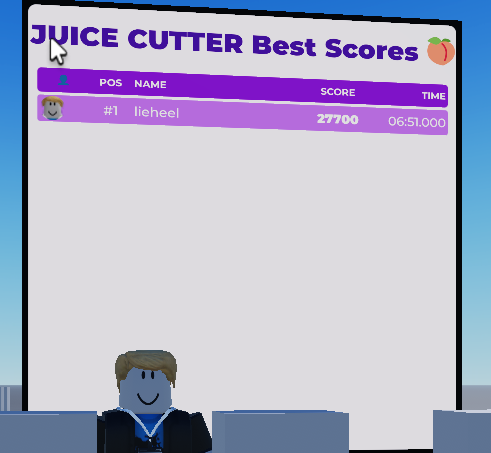
\includegraphics[width=0.6\textwidth]{desarrollo/j6.png}
    \caption*{\textbf{Global Score Table}}
\end{figure}

\clearpage

\subsection{Turris Casei}

Turris Casei is a 3D stacking game built inside Roblox Studio. A block swings back and forth above the tower, and the player has to drop it at the right moment so it lands as well as possible on the block below. If it does not line up, the part that sticks out is cut off, and the landing area gets a little smaller for the next block. There were two main challenges. The first was the slicing math, which figures out the overlap between two blocks instantly using only simple arithmetic. The second was the multiplayer lobby, with private rooms protected by a PIN, live scores shared with everyone in the room, a spectator mode, and the option for the host to kick players.

\subsubsection{Rules of Turris Casei}
\begin{itemize}
  \item \textbf{Main Goal:} Stack blocks as high as possible without losing the platform.
  \item \textbf{Controls (PC):} Space or click to drop the block. Also adapted for mobile touchscreen, Xbox, and PlayStation controllers via \texttt{UniversalController}.
  \item \textbf{Block Oscillation:} The active block swings sinusoidally at a fixed speed of 25 units/s. Its horizontal position is $\sin(t \times 2.5) \times \text{limit}$.
  \item \textbf{Perfect Landing:} If the misalignment on the active axis is $\leq 1.8$ studs, the block snaps to a perfect placement and no trimming occurs.
  \item \textbf{Slicing:} Any overhang beyond the tolerance is trimmed. The remaining block inherits the overlap area. If the block misses entirely, the session ends.
  \item \textbf{Block Types (weighted random):}
  \begin{itemize}
    \item Normal (74\%): no size change, no score bonus.
    \item Good (12.5\%): +1 to size and score.
    \item Good Bonus (3.5\%): +2 to +5 size and score (rarer values are rarer).
    \item Bad (10\%): $-0.5$ size, $-1$ score penalty.
  \end{itemize}
  \item \textbf{Max Block Size:} Capped at 7 studs regardless of bonuses.
  \item \textbf{Multiplayer:} A room host creates a PIN protected lobby (four digit, up to 50 players, 300\,s timeout). Guests join by PIN. The host can kick players, start the match, or spectate others. Live scores are broadcast to all room members during the match.
  \item \textbf{End Condition:} A block that misses the platform entirely ends the player's session. In multiplayer, the last survivor wins.
\end{itemize}

\textbf{Flowchart}
\begin{figure}[H]
  \centering
  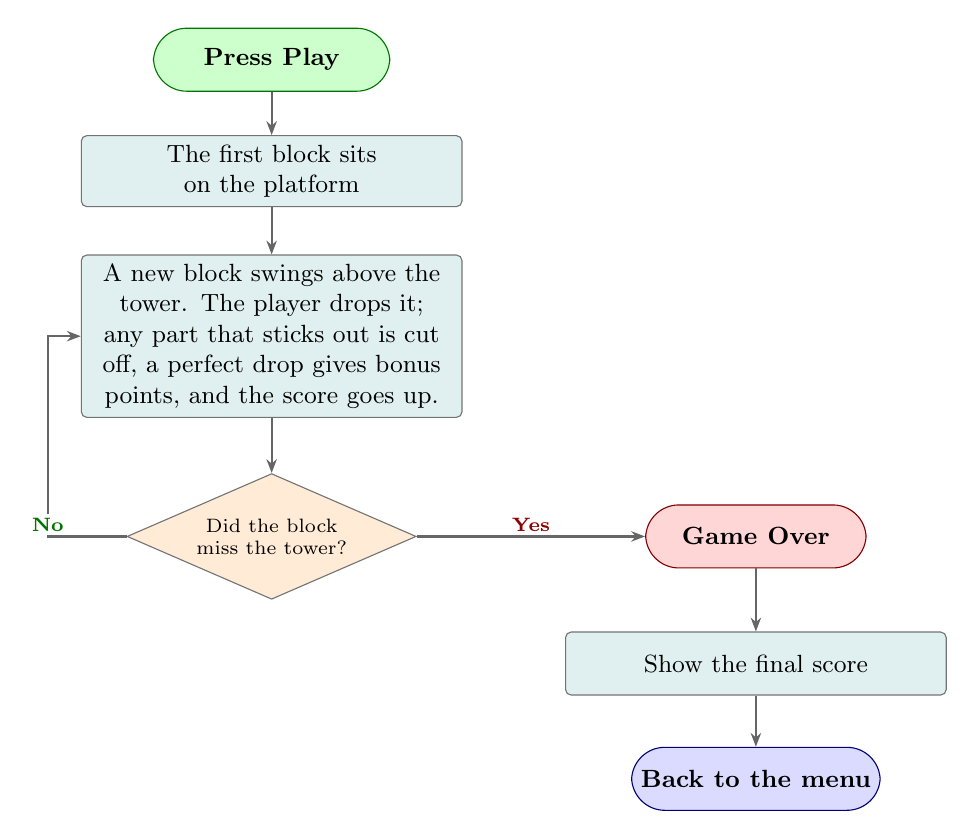
\begin{tikzpicture}[
  font=\small,
  >={Stealth[length=5pt]},
  start/.style={rectangle, rounded corners=12pt, draw=green!45!black, fill=green!20,
                minimum width=3cm, minimum height=0.8cm, align=center, font=\small\bfseries},
  menu/.style={rectangle, rounded corners=12pt, draw=blue!45!black, fill=blue!14,
               minimum width=3cm, minimum height=0.8cm, align=center, font=\small\bfseries},
  over/.style={rectangle, rounded corners=12pt, draw=red!50!black, fill=red!16,
               minimum width=2.8cm, minimum height=0.8cm, align=center, font=\small\bfseries},
  act/.style={rectangle, draw=black!55, fill=teal!12, rounded corners=2pt,
              text width=4.6cm, minimum height=0.8cm, align=center},
  dec/.style={diamond, draw=black!55, fill=orange!16, aspect=2.3,
              align=center, inner sep=1pt, text width=2.4cm, font=\scriptsize},
  link/.style={->, thick, draw=black!60},
  yeslbl/.style={font=\scriptsize\bfseries, color=green!45!black, fill=white, inner sep=1.5pt},
  nolbl/.style={font=\scriptsize\bfseries, color=red!55!black, fill=white, inner sep=1.5pt},
]

\node[start] (s) {Press Play};
\node[act, below=0.55cm of s]   (init) {The first block sits on the platform};
\node[act, below=0.6cm of init] (play) {A new block swings above the tower. The player drops it; any part that sticks out is cut off, a perfect drop gives bonus points, and the score goes up.};
\node[dec, below=0.7cm of play] (miss) {Did the block miss the tower?};

\node[over, right=2.9cm of miss]   (go)   {Game Over};
\node[act, below=0.8cm of go]      (score){Show the final score};
\node[menu, below=0.65cm of score] (back) {Back to the menu};

\draw[link] (s) -- (init);
\draw[link] (init) -- (play);
\draw[link] (play) -- (miss);
\draw[link] (miss.east) -- node[nolbl, above]{Yes} (go.west);
\draw[link] (miss.west) -- ++(-1.0,0) node[yeslbl, above]{No} |- (play.west);
\draw[link] (go) -- (score);
\draw[link] (score) -- (back);

\end{tikzpicture}

  \caption{Flowchart for Turris Casei.}
  \label{fig:turriscasei_flow}
\end{figure}

\subsubsection{Project Structure}

Turris Casei has a more complex server layout than the other games because it needs a dedicated match manager module for the multiplayer lobby.

\begin{lstlisting}
TurrisCasei/
|-- Workspace/
|   +-- TurrisCasei/ (Folder)
|       +-- ButtonTurrisCasei          (Part, Tag="TurrisTerminal")
|-- ReplicatedStorage/
|   |-- ArcadeRemotes/
|   |   +-- TurrisCasei/ (Folder)
|   |       |-- StartTurrisCaseiRequest    (RemoteEvent)
|   |       |-- MatchStatus               (RemoteEvent)
|   |       |-- ToggleAudio               (RemoteEvent)
|   |       |-- UpdateTurrisCaseiLeaderboard (RemoteEvent)
|   |       |-- GetAudioState             (RemoteFunction)
|   |       +-- LobbySystem/ (Folder)
|   |           |-- CreateRoom            (RemoteFunction)
|   |           |-- JoinRoom              (RemoteFunction)
|   |           |-- StartMultiplayerMatch (RemoteEvent)
|   |           |-- RoomUpdate            (RemoteEvent)
|   |           |-- KickPlayer            (RemoteEvent)
|   |           |-- LeaveRoom             (RemoteEvent)
|   |           |-- UpdateLiveScore       (RemoteEvent)
|   |           |-- SpectateTarget        (RemoteEvent)
|   |           +-- PlayerDied            (RemoteEvent)
|   +-- Modules/
|       +-- TurrisCaseiModule          (ModuleScript)
|-- ServerScriptService/
|   |-- TurrisCaseiServer              (Script)
|   +-- TurrisCaseiMatchManager        (ModuleScript)
+-- StarterPlayer/
    +-- StarterPlayerScripts/
        +-- TurrisCaseiClient          (LocalScript)
\end{lstlisting}

\subsubsection{Time Complexity}

Every important step in the game runs in $O(1)$ time, meaning it always costs the same small amount no matter how tall the tower gets. Working out where the block is in its swing is a single calculation. Choosing the next block is one random draw plus a few checks. Working out the overlap between two blocks uses only subtractions and comparisons on a handful of numbers. There are no loops and nothing that grows while playing. The multiplayer match manager does keep a table for the room with up to 50 players, but the work done each time a block drops stays $O(1)$.

\subsubsection{Space Complexity}

The memory the game logic uses is $O(1)$. To place a block, the game only needs the position and size of the previous block and the position of the current one, which are just a few numbers. It does not keep a history of the blocks already placed. The match manager keeps some data for each room (the player list, the score table, who is spectating) for up to 50 players, but that does not depend on how many blocks have been stacked.

\subsubsection{Game Features and Implementation Status}

\begin{table}[H]
\centering
\begin{tabular}{|p{4cm}|p{8cm}|p{2.5cm}|}
\hline
\textbf{Feature} & \textbf{Description} & \textbf{Status} \\
\hline
Main Menu & Interface with Play, VIP, and Exit buttons. & Working \\
\hline
Menu Sounds & Audio feedback for navigation and selection. & Working \\
\hline
Gameplay Controls & One button drop (Space or click/tap). & Working \\
\hline
Mute Button & In game toggle to turn all audio on or off. & Working \\
\hline
Exit Button (Game) & Allows the player to abort the run and return to the score menu. & Working \\
\hline
Score Menu & A screen after the game showing the final score and a replay option. & Working \\
\hline
Block Slicing Logic & $O(1)$ overlap calculation using axis aligned coordinate arithmetic. Trims overhang to the shared area. & Working \\
\hline
Block Types & Weighted random draw each drop: Normal 74\%, Good 12.5\%, Good Bonus 3.5\%, Bad 10\%. & Working \\
\hline
Perfect Landing & Misalignment $\leq 1.8$ studs snaps to center with no size loss. & Working \\
\hline
Multiplayer Lobby & PIN protected rooms (four digit), up to 50 players, 300\,s timeout, host kick controls. & Working \\
\hline
Live Score Broadcast & Real time score table sent to all room members after every block drop. & Working \\
\hline
Spectator Mode & Players eliminated from the match can spectate any surviving participant. & Working \\
\hline
Anti AFK & Inactivity detection to prevent stalling in multiplayer matches. & Working \\
\hline
Top 10 Score Table & Global leaderboard via Roblox DataStore. & Working \\
\hline
VIP Donation Menu & Opens a menu with various donation tiers. & Working \\
\hline
Optimization & $O(1)$ per block drop; $O(P)$ lobby data with $P \leq 50$ players. & Working \\
\hline
Mobile Adaptation & Touchscreen input via \texttt{UniversalController}. & Working \\
\hline
Xbox Adaptation & Gamepad input via \texttt{UniversalController}. & Working \\
\hline
PlayStation Adaptation & DualSense and DualShock input via \texttt{UniversalController}. & Working \\
\hline
\end{tabular}
\caption{Functionalities and current status of Turris Casei.}
\end{table}

\subsubsection{Game Results}

\begin{figure}[H]
    \centering
    \begin{minipage}[b]{0.32\textwidth}
        \centering
        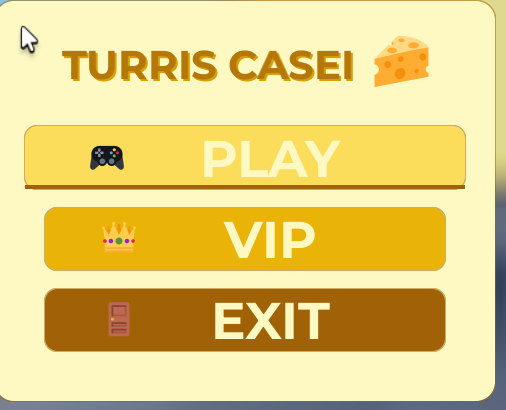
\includegraphics[width=\linewidth]{desarrollo/tu1.png}
        \caption*{\textbf{Main Menu}}
    \end{minipage}
    \hfill
    \begin{minipage}[b]{0.32\textwidth}
        \centering
        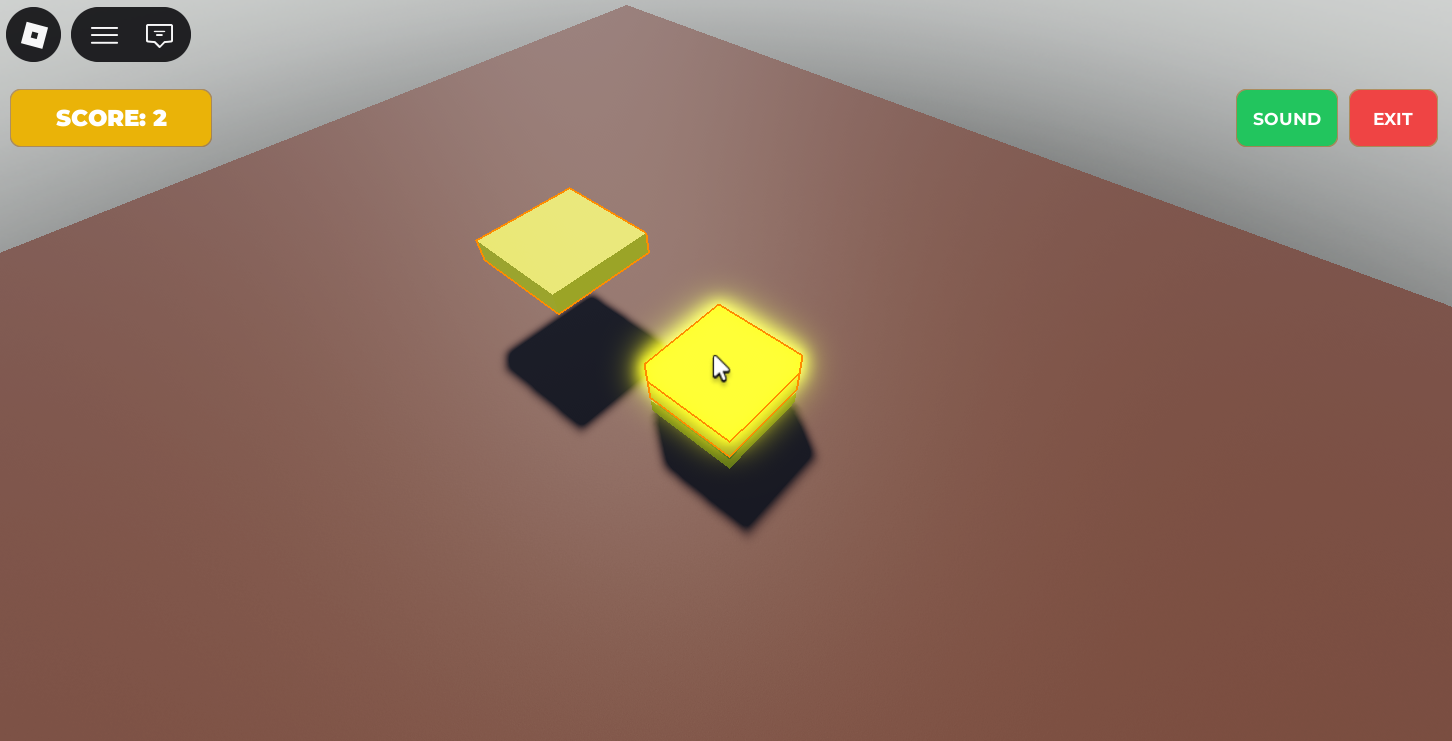
\includegraphics[width=\linewidth]{desarrollo/tu2.png}
        \caption*{\textbf{Gameplay}}
    \end{minipage}
    \hfill
    \begin{minipage}[b]{0.32\textwidth}
        \centering
        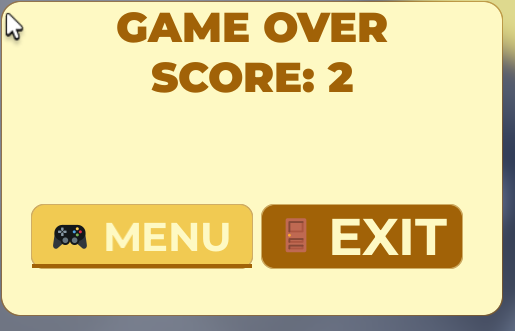
\includegraphics[width=\linewidth]{desarrollo/tu3.png}
        \caption*{\textbf{Score Menu}}
    \end{minipage}
\end{figure}

\begin{figure}[H]
    \centering
    \begin{minipage}[b]{0.47\textwidth}
        \centering
        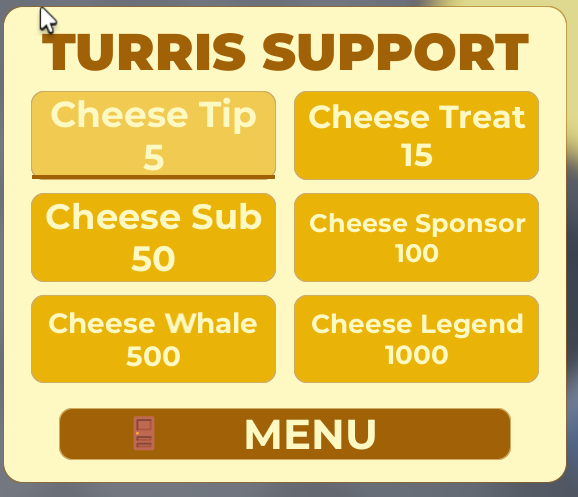
\includegraphics[width=\linewidth]{desarrollo/tu4.png}
        \caption*{\textbf{VIP Menu}}
    \end{minipage}
    \hfill
    \begin{minipage}[b]{0.47\textwidth}
        \centering
        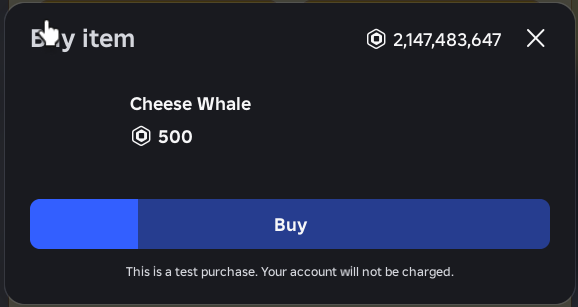
\includegraphics[width=\linewidth]{desarrollo/tu5.png}
        \caption*{\textbf{Donation Interface}}
    \end{minipage}
\end{figure}

\begin{figure}[H]
    \centering
    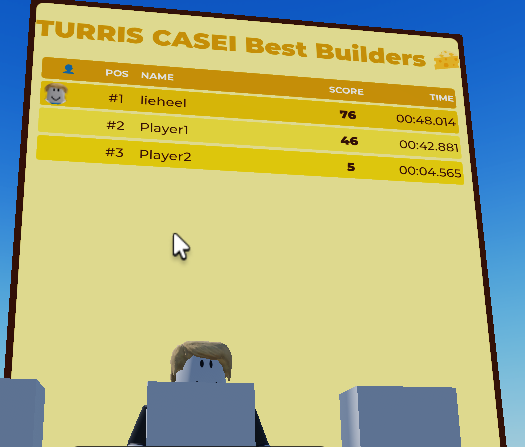
\includegraphics[width=0.6\textwidth]{desarrollo/tu6.png}
    \caption*{\textbf{Global Score Table}}
\end{figure}

\begin{figure}[H]
    \centering
    \begin{minipage}[b]{0.47\textwidth}
        \centering
        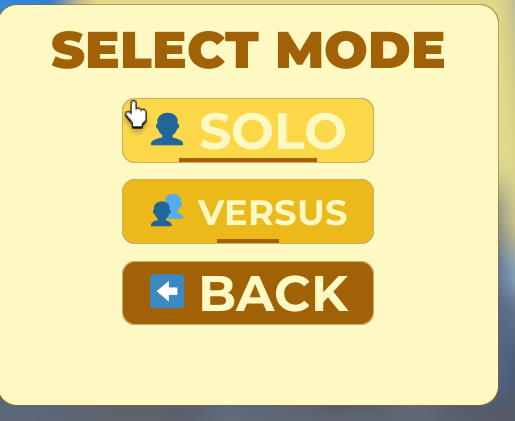
\includegraphics[width=\linewidth]{desarrollo/tu7.png}
    \end{minipage}
    \hfill
    \begin{minipage}[b]{0.47\textwidth}
        \centering
        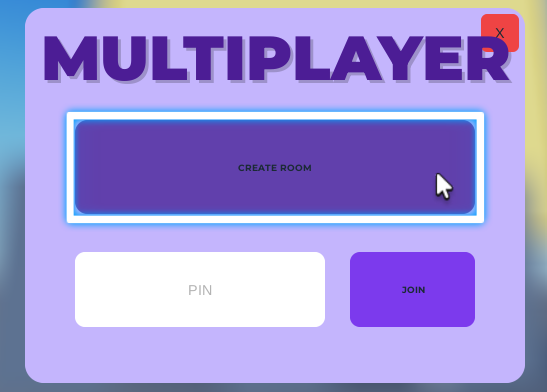
\includegraphics[width=\linewidth]{desarrollo/tu8.png}
    \end{minipage}
    \vspace{0.5cm}
    \begin{minipage}[b]{0.47\textwidth}
        \centering
        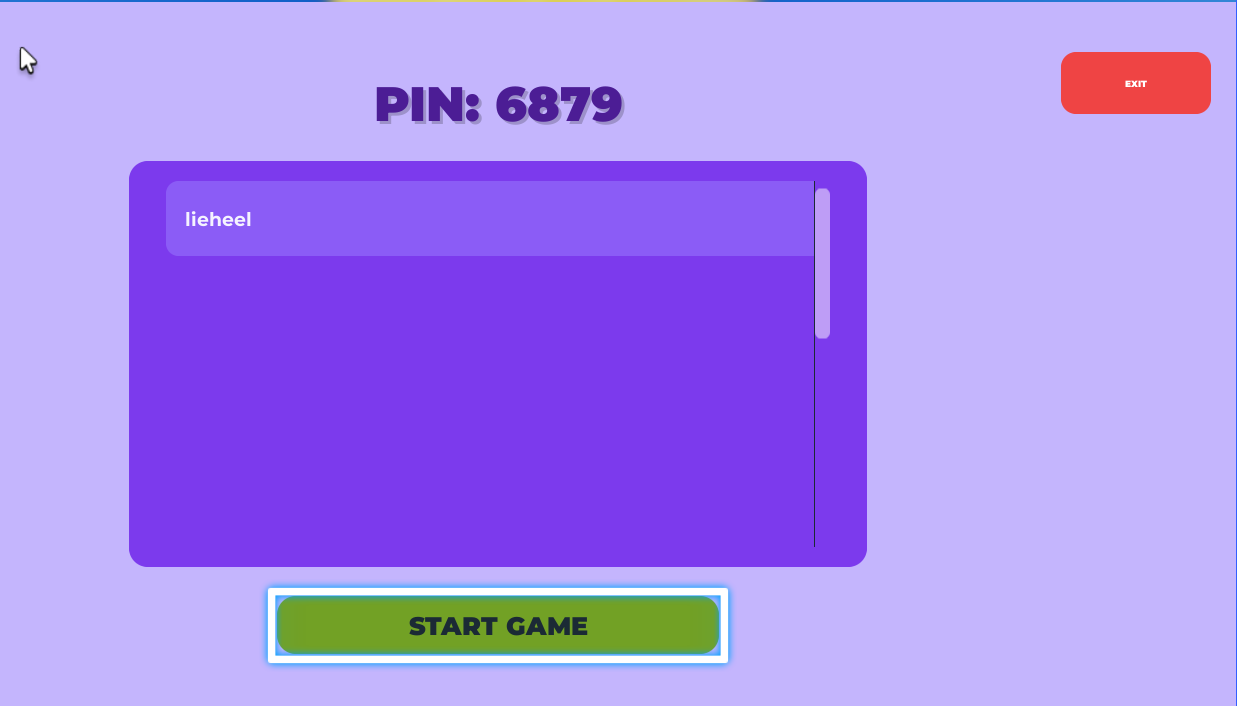
\includegraphics[width=\linewidth]{desarrollo/tu9.png}
    \end{minipage}
    \hfill
    \begin{minipage}[b]{0.47\textwidth}
        \centering
        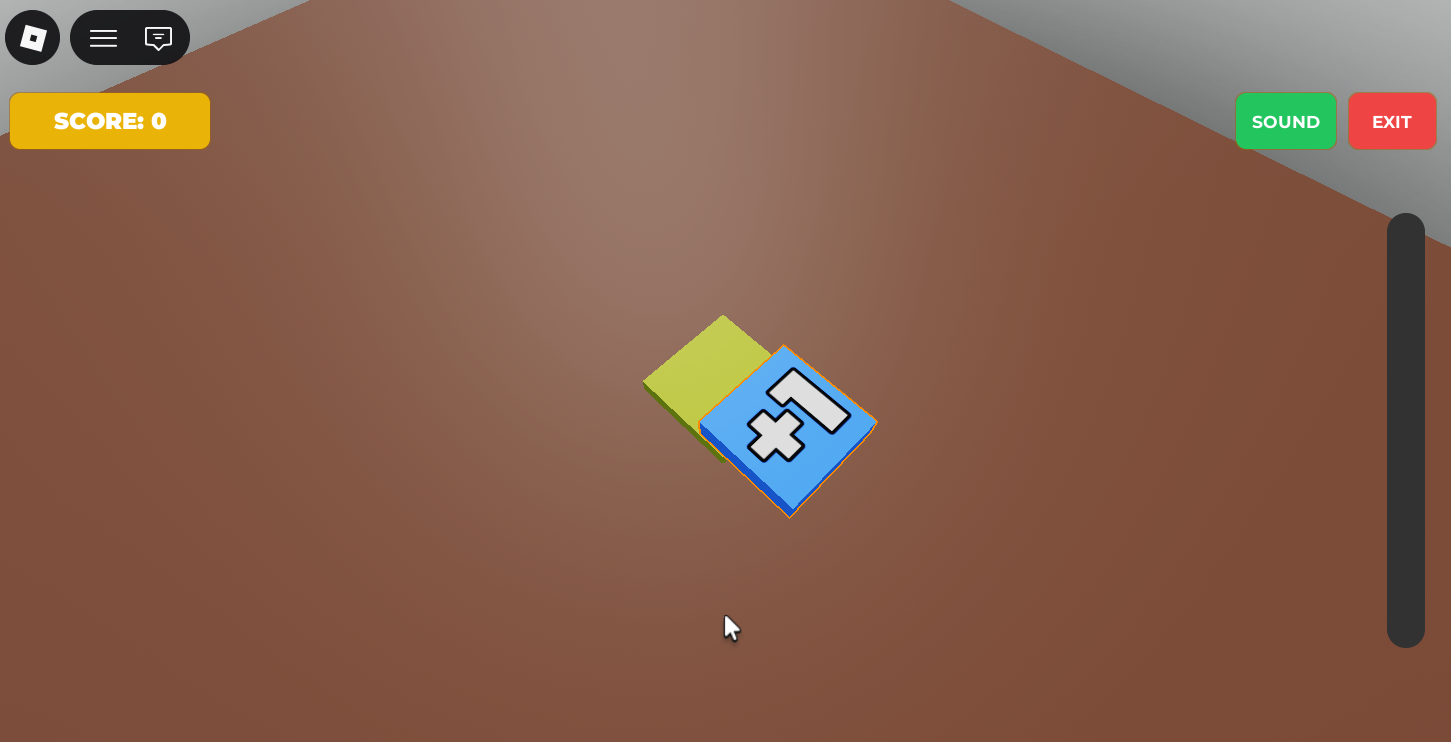
\includegraphics[width=\linewidth]{desarrollo/tu10.png}
    \end{minipage}
    \caption{Multiplayer Lobby System: PIN entry, room creation, and versus mode.}
\end{figure}

\clearpage

\subsection{Tap And Hold}

Tap And Hold is a 3D jumping game built inside Roblox Studio. The player holds a button to charge a jump and lets go to send the character flying in a curve toward the next platform. The longer the hold, the farther the jump, up to a maximum charge of about 1.1 seconds. The platforms are created on the fly in a zigzag, with at most 4 visible at a time, and the old ones are removed as the player moves forward. The multiplayer works the same way as in Turris Casei: private rooms protected by a PIN, live scores after every jump, a spectator mode for players who fall, and the option for the host to kick players.

\subsubsection{Rules of Tap And Hold}
\begin{itemize}
  \item \textbf{Main Goal:} Reach as many platforms as possible without falling.
  \item \textbf{Controls (PC):} Hold Space or click to charge the jump; release to launch. Also adapted for mobile touchscreen, Xbox, and PlayStation controllers via \texttt{UniversalController}.
  \item \textbf{Jump Physics:} Hold time is converted to power: $\text{power} = \min(\text{holdTime} \times 45,\; 50)$. Forward velocity is $\text{power} \times 2.2$ and upward velocity is $35 + \text{power} \times 0.2$. Gravity is set to 196.2 studs/s\textsuperscript{2}.
  \item \textbf{Perfect Landing:} Landing within 1.2 studs of the platform center awards a perfect bonus and triggers a visual highlight.
  \item \textbf{Platform Events (per platform, random):}
  \begin{itemize}
    \item Normal (80\%): no score modifier.
    \item Bonus (10\%): $+5$ score on landing.
    \item Penalty (10\%): $-1$ score on landing.
  \end{itemize}
  \item \textbf{Platform Generation:} Platforms are chosen from four weighted models (tapsuelo1 and tapsuelo2 at 32.5\% each, tapsuelo3 and tapsuelo4 at 17.5\% each) and placed in a zigzag pattern between 8 and 22 studs apart. At most 4 platforms exist in the world at any instant; the oldest is destroyed when a new one spawns.
  \item \textbf{Multiplayer:} PIN protected rooms (four digit), up to 50 players, 300\,s lobby timeout. The host can kick players, start the match, or spectate others. Live scores are broadcast to all room members after every jump.
  \item \textbf{End Condition:} Falling off a platform ends the player's session. In multiplayer, the last survivor wins.
\end{itemize}

\textbf{Flowchart}
\begin{figure}[H]
  \centering
  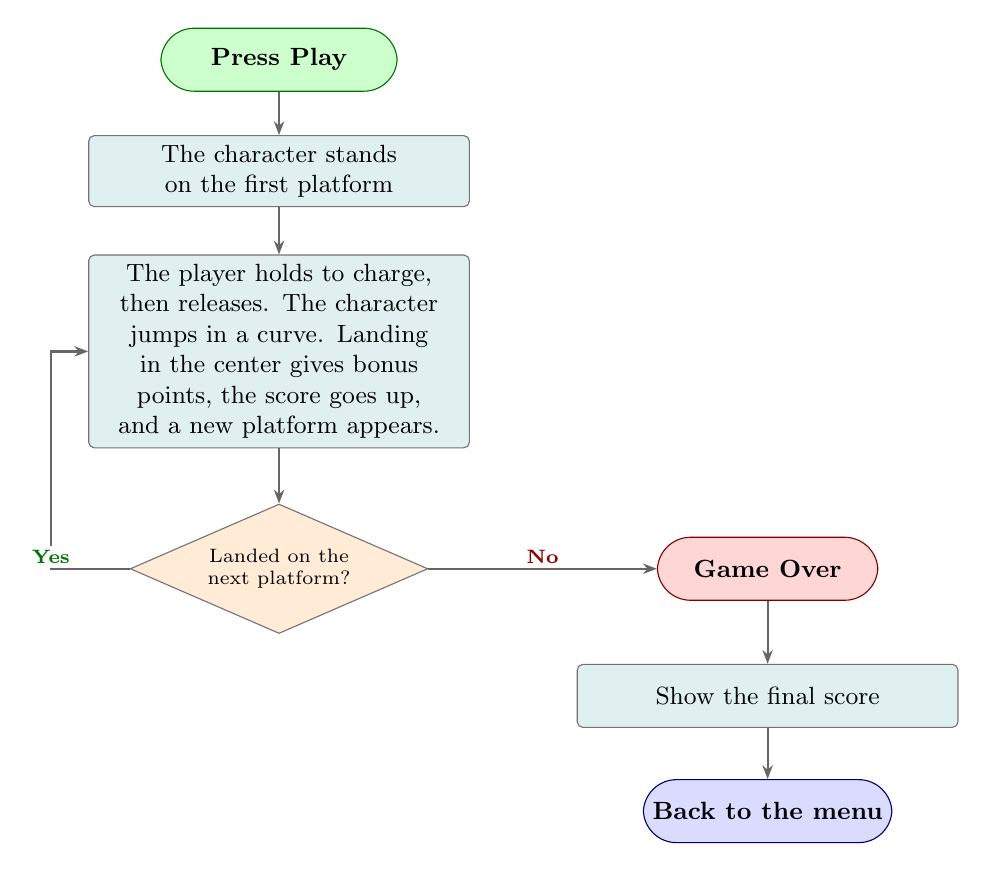
\begin{tikzpicture}[
  font=\small,
  >={Stealth[length=5pt]},
  start/.style={rectangle, rounded corners=12pt, draw=green!45!black, fill=green!20,
                minimum width=3cm, minimum height=0.8cm, align=center, font=\small\bfseries},
  menu/.style={rectangle, rounded corners=12pt, draw=blue!45!black, fill=blue!14,
               minimum width=3cm, minimum height=0.8cm, align=center, font=\small\bfseries},
  over/.style={rectangle, rounded corners=12pt, draw=red!50!black, fill=red!16,
               minimum width=2.8cm, minimum height=0.8cm, align=center, font=\small\bfseries},
  act/.style={rectangle, draw=black!55, fill=teal!12, rounded corners=2pt,
              text width=4.6cm, minimum height=0.8cm, align=center},
  dec/.style={diamond, draw=black!55, fill=orange!16, aspect=2.3,
              align=center, inner sep=1pt, text width=2.4cm, font=\scriptsize},
  link/.style={->, thick, draw=black!60},
  yeslbl/.style={font=\scriptsize\bfseries, color=green!45!black, fill=white, inner sep=1.5pt},
  nolbl/.style={font=\scriptsize\bfseries, color=red!55!black, fill=white, inner sep=1.5pt},
]

\node[start] (s) {Press Play};
\node[act, below=0.55cm of s]   (init) {The character stands on the first platform};
\node[act, below=0.6cm of init] (play) {The player holds to charge, then releases. The character jumps in a curve. Landing in the center gives bonus points, the score goes up, and a new platform appears.};
\node[dec, below=0.7cm of play] (land) {Landed on the next platform?};

\node[over, right=2.9cm of land]   (go)   {Game Over};
\node[act, below=0.8cm of go]      (score){Show the final score};
\node[menu, below=0.65cm of score] (back) {Back to the menu};

\draw[link] (s) -- (init);
\draw[link] (init) -- (play);
\draw[link] (play) -- (land);
\draw[link] (land.east) -- node[nolbl, above]{No} (go.west);
\draw[link] (land.west) -- ++(-1.0,0) node[yeslbl, above]{Yes} |- (play.west);
\draw[link] (go) -- (score);
\draw[link] (score) -- (back);

\end{tikzpicture}

  \caption{Flowchart for Tap And Hold.}
  \label{fig:tapandhold_flow}
\end{figure}

\subsubsection{Project Structure}

Tap And Hold shares the same expanded server layout as Turris Casei, with a dedicated match manager and separate leaderboard client.

\begin{lstlisting}
TapAndHold/
|-- Workspace/
|   +-- TapAndHold/ (Folder)
|       +-- ButtonTapAndHold           (Part, Tag="TapAndHoldTerminal")
|-- ReplicatedStorage/
|   |-- ArcadeRemotes/
|   |   +-- TapAndHold/ (Folder)
|   |       |-- StartTapAndHoldRequest     (RemoteEvent)
|   |       |-- SubmitJumpCharge           (RemoteEvent)
|   |       |-- MatchStatus               (RemoteEvent)
|   |       |-- ToggleAudio               (RemoteEvent)
|   |       |-- UpdateTapAndHoldLeaderboard (RemoteEvent)
|   |       |-- GetAudioState             (RemoteFunction)
|   |       +-- LobbySystem/ (Folder)
|   |           |-- CreateRoom            (RemoteFunction)
|   |           |-- JoinRoom              (RemoteFunction)
|   |           |-- StartMultiplayerMatch (RemoteEvent)
|   |           |-- RoomUpdate            (RemoteEvent)
|   |           |-- KickPlayer            (RemoteEvent)
|   |           |-- LeaveRoom             (RemoteEvent)
|   |           |-- UpdateLiveScore       (RemoteEvent)
|   |           |-- SpectateTarget        (RemoteEvent)
|   |           +-- PlayerDied            (RemoteEvent)
|   |-- TapAndHold_Assets/ (Folder)
|   |   |-- tapsuelo1, tapsuelo2          (Platform models)
|   |   |-- tapsuelo3, tapsuelo4          (Platform models)
|   |   +-- Model                         (Floor model)
|   +-- Modules/
|       +-- TapAndHoldModule           (ModuleScript)
|-- ServerScriptService/
|   |-- TapAndHoldServer               (Script)
|   +-- TapAndHoldMatchManager         (ModuleScript)
+-- StarterPlayer/
    +-- StarterPlayerScripts/
        +-- TapAndHoldClient           (LocalScript)
\end{lstlisting}

\subsubsection{Time Complexity}

Every step in the game runs in $O(1)$ time, always costing the same small amount no matter how far the player gets. Turning the hold time into a jump is two short calculations. Checking the landing is a few comparisons and one distance. Choosing the next platform goes through a fixed list of 4 platform types plus one extra roll. Creating a new platform works out one coordinate and removes the oldest one from a list that never holds more than 4. The match manager keeps some data for the room with up to 50 players, but the work done on each jump stays $O(1)$.

\subsubsection{Space Complexity}

The memory the game logic uses is $O(1)$. There are never more than 4 platforms in the world at once, and the oldest one is removed whenever a new one appears. Checking a landing only needs the character's position and the current platform's position and size. Turning the hold into a jump uses just a couple of numbers. The match manager keeps some data for each room (the player list, the score table, who is spectating) for up to 50 players, and that does not depend on how many jumps the player has made.

\subsubsection{Game Features and Implementation Status}

\begin{table}[H]
\centering
\begin{tabular}{|p{4cm}|p{8cm}|p{2.5cm}|}
\hline
\textbf{Feature} & \textbf{Description} & \textbf{Status} \\
\hline
Main Menu & Interface with Play, VIP, and Exit buttons. & Working \\
\hline
Menu Sounds & Audio feedback for navigation and selection. & Working \\
\hline
Gameplay Controls & Hold to charge jump, release to launch in a parabolic arc. & Working \\
\hline
Mute Button & In game toggle to turn all audio on or off. & Working \\
\hline
Exit Button (Game) & Allows the player to abort the run and return to the score menu. & Working \\
\hline
Score Menu & A screen after the game showing the final score and a replay option. & Working \\
\hline
Parabolic Jump Physics & Hold time converted to forward ($\times 2.2$) and upward ($35 + \times 0.2$) velocity; gravity 196.2\,studs/s\textsuperscript{2}. & Working \\
\hline
Perfect Landing & Landing within 1.2 studs of center triggers a visual effect and bonus score. & Working \\
\hline
Platform Events & Random per platform: Normal 80\%, Bonus $+5$ (10\%), Penalty $-1$ (10\%). & Working \\
\hline
Infinite Platform Generation & Procedural zigzag spawning from 4 weighted models; at most 4 visible at any time, oldest destroyed on spawn. & Working \\
\hline
Multiplayer Lobby & PIN protected rooms (four digit), up to 50 players, 300\,s timeout, host kick controls. & Working \\
\hline
Live Score Broadcast & Real time score table sent to all room members after every jump. & Working \\
\hline
Spectator Mode & Players who fall can spectate any surviving participant. & Working \\
\hline
Anti AFK & Inactivity detection to prevent stalling in multiplayer matches. & Working \\
\hline
Top 10 Score Table & Global leaderboard via Roblox DataStore. & Working \\
\hline
VIP Donation Menu & Opens a menu with various donation tiers. & Working \\
\hline
Optimization & $O(1)$ per jump; max 4 platforms in memory at any time. & Working \\
\hline
Mobile Adaptation & Touchscreen hold and release input via \texttt{UniversalController}. & Working \\
\hline
Xbox Adaptation & Gamepad button hold via \texttt{UniversalController}. & Working \\
\hline
PlayStation Adaptation & DualSense and DualShock hold input via \texttt{UniversalController}. & Working \\
\hline
\end{tabular}
\caption{Functionalities and current status of Tap And Hold.}
\end{table}

\subsubsection{Game Results}

\begin{figure}[H]
    \centering
    \begin{minipage}[b]{0.32\textwidth}
        \centering
        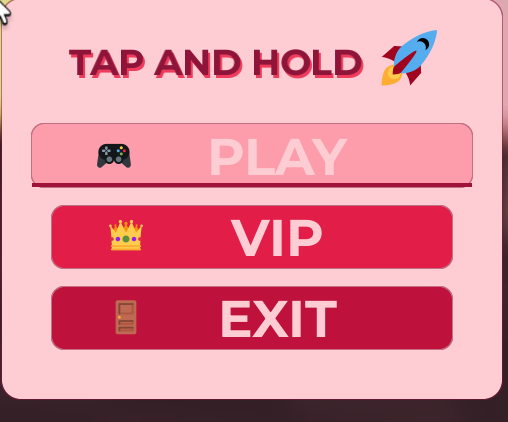
\includegraphics[width=\linewidth]{desarrollo/tap1.png}
        \caption*{\textbf{Main Menu}}
    \end{minipage}
    \hfill
    \begin{minipage}[b]{0.32\textwidth}
        \centering
        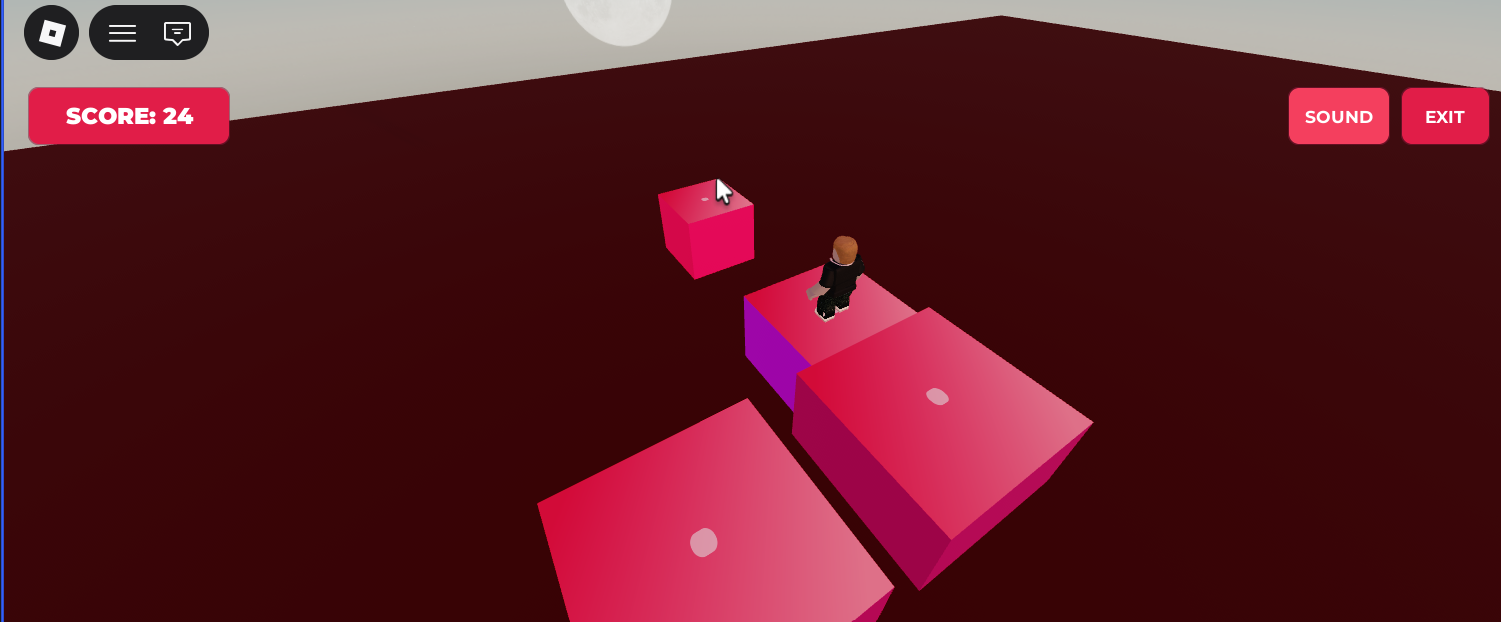
\includegraphics[width=\linewidth]{desarrollo/tap2.png}
        \caption*{\textbf{Gameplay}}
    \end{minipage}
    \hfill
    \begin{minipage}[b]{0.32\textwidth}
        \centering
        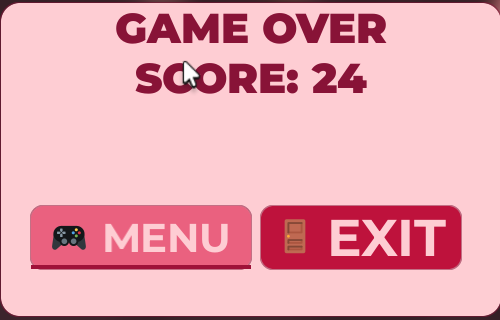
\includegraphics[width=\linewidth]{desarrollo/tap3.png}
        \caption*{\textbf{Score Menu}}
    \end{minipage}
\end{figure}

\begin{figure}[H]
    \centering
    \begin{minipage}[b]{0.47\textwidth}
        \centering
        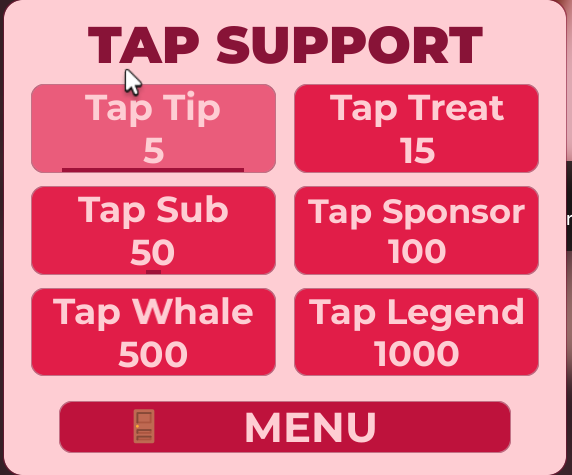
\includegraphics[width=\linewidth]{desarrollo/tap4.png}
        \caption*{\textbf{Play Mode Menu}}
    \end{minipage}
    \hfill
    \begin{minipage}[b]{0.47\textwidth}
        \centering
        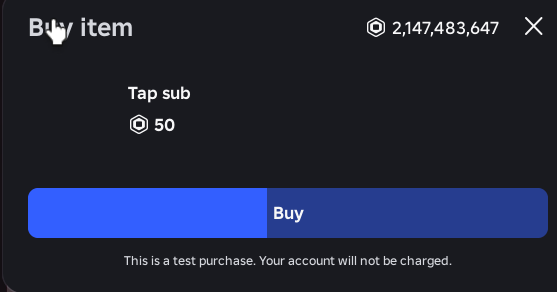
\includegraphics[width=\linewidth]{desarrollo/tap5.png}
        \caption*{\textbf{Donation Interface}}
    \end{minipage}
\end{figure}

\begin{figure}[H]
    \centering
    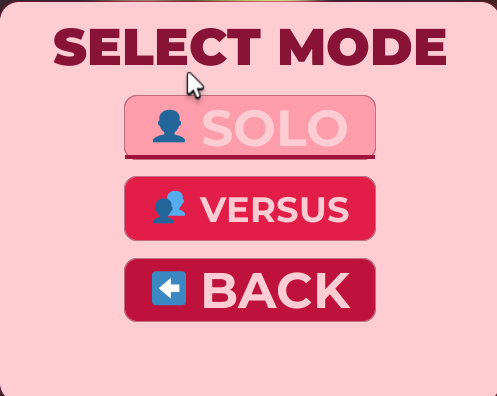
\includegraphics[width=0.6\textwidth]{desarrollo/tap6.png}
    \caption*{\textbf{Global Score Table}}
\end{figure}

\begin{figure}[H]
    \centering
    \begin{minipage}[b]{0.32\textwidth}
        \centering
        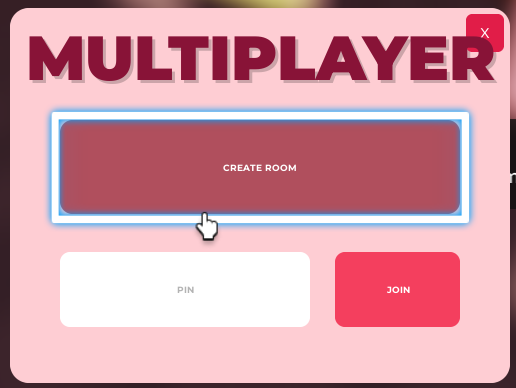
\includegraphics[width=\linewidth]{desarrollo/tap7.png}
    \end{minipage}
    \hfill
    \begin{minipage}[b]{0.32\textwidth}
        \centering
        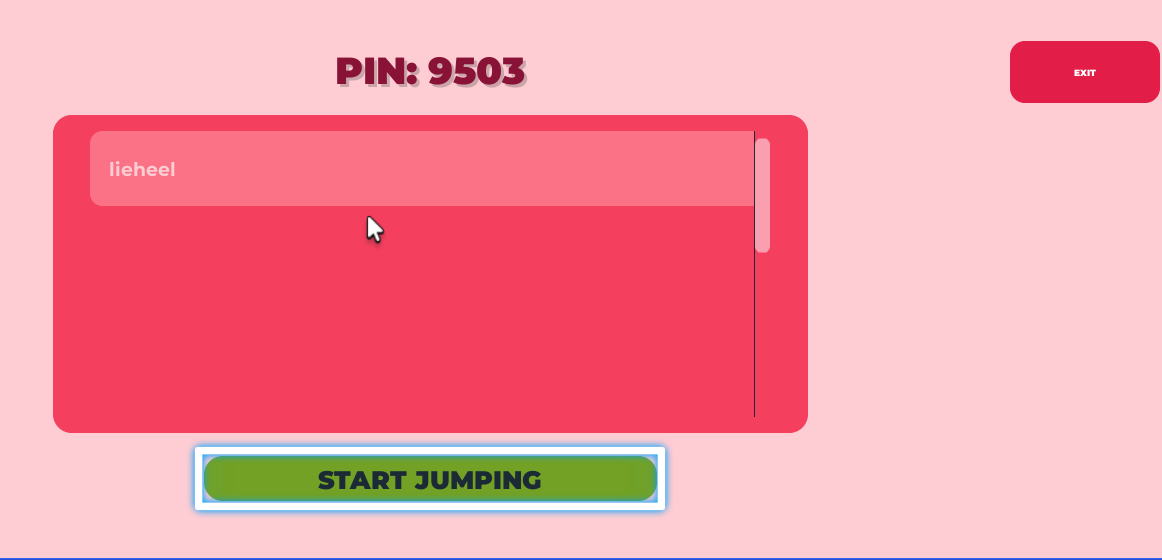
\includegraphics[width=\linewidth]{desarrollo/tap8.png}
    \end{minipage}
    \hfill
    \begin{minipage}[b]{0.32\textwidth}
        \centering
        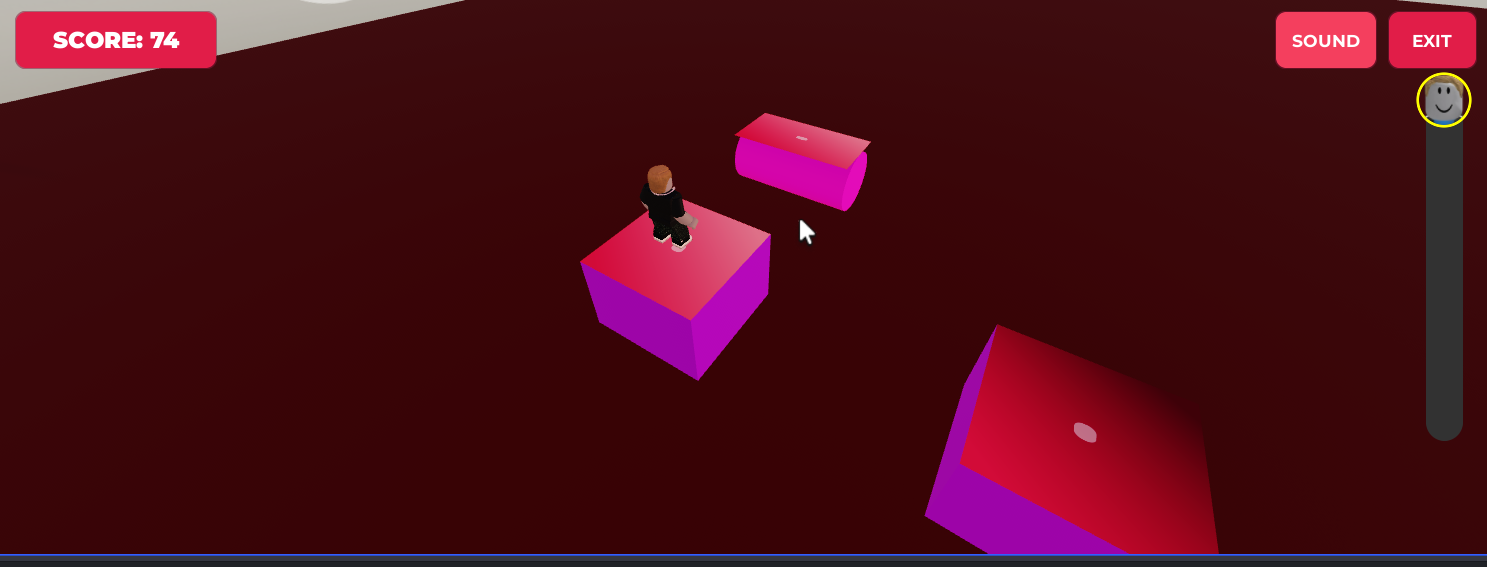
\includegraphics[width=\linewidth]{desarrollo/tap9.png}
    \end{minipage}
    \caption{Multiplayer Lobby System: PIN entry, room creation, and versus mode.}
\end{figure}

\clearpage

\subsection{ImNotASphere}

ImNotASphere is a 3D ball platformer built inside Roblox Studio. The player rolls a sphere through three levels, each one with moving platforms, elevators, coins to collect, kill zones, and a finish line. There are also four power ups that change the speed, the size, the jump height, or let the ball float for a moment, plus a multiplayer lobby. The hard part to build was the ball physics, written from scratch: the module works out the push on the ball, how much control the player has in the air, how the ball rolls, and how far the elevators travel, all without using Roblox's normal character movement.

\subsubsection{Rules of ImNotASphere}
\begin{itemize}
  \item \textbf{Main Goal:} Collect all four required Bitcoin coins on each of the three levels and reach the finish line.
  \item \textbf{Controls (PC):} WASD or arrow keys to roll the sphere, Space to jump. Also adapted for mobile touchscreen, Xbox, and PlayStation controllers via \texttt{UniversalController}.
  \item \textbf{Physics:} The sphere is driven by a custom force model. On the ground, acceleration is 80 units/s\textsuperscript{2} up to a top speed of 40 units/s, with braking deceleration of 60 units/s\textsuperscript{2}. In the air, only 50\% of the ground acceleration is available (AirControl = 0.5). Jump impulse is 50 units $\times$ mass.
  \item \textbf{Collectibles:} Standard Bitcoin coins score 5 points. Super Bitcoin coins score 15 points. Collecting all four required Bitcoins on a level unlocks the finish line.
  \item \textbf{Power ups (respawn every 5\,s):}
  \begin{itemize}
    \item Fast: 1.5\,s duration, speed $\times 3$, acceleration $\times 2.5$.
    \item Big: 6.0\,s duration, sphere size $\times 2.5$.
    \item Wings (ALAS): 3.5\,s duration, magnetic levitation up to 20 studs with spring force 30 and damping 8.
    \item Spring: 2.0\,s duration, jump impulse $\times 2$.
  \end{itemize}
  \item \textbf{Levels:} Three handmade levels, each containing geometry, moving platforms with elevator systems, collectibles, kill zones (death pit below the level), a spawn point, and a finish line.
  \item \textbf{Lives:} 8 lives total. Falling into a kill zone or off the level costs one life.
  \item \textbf{Multiplayer:} PIN protected rooms (four digit), up to 10 players, 300\,s lobby timeout, host kick controls, live score broadcasting, and spectator mode for eliminated players.
  \item \textbf{Score Validation:} The server caps accepted scores at 490 and rejects results submitted in under 1 second to prevent exploits.
  \item \textbf{End Condition:} Losing all 8 lives ends the session. Clearing all three levels is a perfect run.
\end{itemize}

\textbf{Flowchart}
\begin{figure}[H]
  \centering
  \input{diagrama/imnotasphere-flow}
  \caption{Flowchart for ImNotASphere.}
  \label{fig:imnotasphere_flow}
\end{figure}

\subsubsection{Project Structure}

ImNotASphere shares the same expanded server layout as Turris Casei and Tap And Hold, with a dedicated match manager and separate leaderboard client.

\begin{lstlisting}
ImNotASphere/
|-- Workspace/
|   +-- ImNotASphere/ (Folder)
|       +-- ButtonImNotASphere     (Part, Tag="ImNotASphereTerminal")
|-- ReplicatedStorage/
|   |-- ArcadeRemotes/
|   |   +-- ImNotASphere/ (Folder)
|   |       |-- StartImNotASphereRequest   (RemoteEvent)
|   |       |-- MatchStatus               (RemoteEvent)
|   |       |-- ToggleAudio               (RemoteEvent)
|   |       |-- UpdateImNotASphereLeaderboard (RemoteEvent)
|   |       |-- GetAudioState             (RemoteFunction)
|   |       +-- LobbySystem/ (Folder)
|   |           |-- CreateRoom            (RemoteFunction)
|   |           |-- JoinRoom              (RemoteFunction)
|   |           |-- StartMultiplayerMatch (RemoteEvent)
|   |           |-- RoomUpdate            (RemoteEvent)
|   |           |-- KickPlayer            (RemoteEvent)
|   |           |-- LeaveRoom             (RemoteEvent)
|   |           |-- UpdateLiveScore       (RemoteEvent)
|   |           |-- SpectateTarget        (RemoteEvent)
|   |           +-- PlayerDied            (RemoteEvent)
|   |-- ImNotASphere_Assets/ (Folder)
|   |   |-- PlayerSphere                  (Part, player ball)
|   |   |-- Level1, Level2, Level3        (Models)
|   |   |   |-- Geometry/                 (Folder, optional)
|   |   |   |-- MovingPlatforms/          (Folder)
|   |   |   |   +-- Elevator1             (Model: Platform + StartPart + EndPart)
|   |   |   |-- Collectibles/             (Folder)
|   |   |   |   |-- Coin                  (Bitcoin, 5 pts)
|   |   |   |   +-- ExtraPoint            (Super Bitcoin, 15 pts)
|   |   |   |-- KillZones/               (Folder)
|   |   |   |   +-- DeathPit             (Transparent part below level)
|   |   |   |-- SpawnPoint               (Transparent part)
|   |   |   +-- FinishLine               (Part, unlocked after 4 Bitcoins)
|   +-- Modules/
|       |-- ImNotASphereModule         (ModuleScript)
|       +-- ImNotASphereLeaderboard    (ModuleScript)
|-- ServerScriptService/
|   |-- ImNotASphereServer             (Script)
|   +-- ImNotASphereMatchManager       (ModuleScript)
+-- StarterPlayer/
    +-- StarterPlayerScripts/
        +-- ImNotASphereClient         (LocalScript)
\end{lstlisting}

\subsubsection{Time Complexity}

Every function in the physics module runs in $O(1)$ time, always costing the same small amount. Working out the push on the ball is a fixed set of operations that checks at most 4 active power ups. Working out how the ball rolls is a single calculation, the jump is one multiplication, and the elevator distance is one subtraction between two points. There are no loops and nothing that grows while playing. The match manager keeps some data for the room with up to 10 players, and that does not depend on how long the game has been running.

\subsubsection{Space Complexity}

The memory the module uses is $O(1)$. The physics module does not store anything of its own: it takes the inputs, returns the result, and keeps no data between calls. The list of active power ups it receives never has more than 4 entries. The real game state (the ball's position and speed, the lives, the coins) lives in the 3D world as Roblox parts, handled by the client. The match manager keeps some data for each room for up to 10 players.

\subsubsection{Game Features and Implementation Status}

\begin{table}[H]
\centering
\begin{tabular}{|p{4cm}|p{8cm}|p{2.5cm}|}
\hline
\textbf{Feature} & \textbf{Description} & \textbf{Status} \\
\hline
Main Menu & Interface with Play, VIP, and Exit buttons. & Working \\
\hline
Menu Sounds & Audio feedback for navigation and selection. & Working \\
\hline
Gameplay Controls & WASD to roll the sphere, Space to jump. & Working \\
\hline
Mute Button & In game toggle to turn all audio on or off. & Working \\
\hline
Exit Button (Game) & Allows the player to abort the run and return to the score menu. & Working \\
\hline
Score Menu & A screen after the game showing the final score and a replay option. & Working \\
\hline
Custom Physics Engine & Force based ball controller: ground acceleration 80, top speed 40, air control 0.5, jump impulse 50. & Working \\
\hline
Level System & Three handmade levels with geometry, moving platforms, elevators, collectibles, kill zones, and finish lines. & Working \\
\hline
Collectible System & Four required Bitcoin coins (5 pts each) unlock the finish line. Super Bitcoin coins score 15 pts. & Working \\
\hline
Power up System & Four power ups: Fast ($\times 3$ speed, 1.5\,s), Big ($\times 2.5$ size, 6\,s), Wings (levitation up to 20 studs, 3.5\,s), Spring ($\times 2$ jump, 2\,s). Respawn every 5\,s. & Working \\
\hline
Elevator System & Moving platforms travel between StartPart and EndPart markers; distance calculated via \texttt{CalculateElevatorLimits}. & Working \\
\hline
Multiplayer Lobby & PIN protected rooms (four digit), up to 10 players, 300\,s timeout, host kick controls. & Working \\
\hline
Live Score Broadcast & Real time score updates sent to all room members. & Working \\
\hline
Spectator Mode & Eliminated players can spectate any surviving participant. & Working \\
\hline
Anti cheat Validation & Server rejects scores above 490 or submitted in under 1 second. & Working \\
\hline
Top 10 Score Table & Global leaderboard via Roblox DataStore. & Working \\
\hline
VIP Donation Menu & Six donation tiers (5 to 1000 Robux) with purchase deduplication via DataStore. & Working \\
\hline
Optimization & $O(1)$ per physics tick; module is stateless with no dynamic allocations. & Working \\
\hline
Mobile Adaptation & Touchscreen input via \texttt{UniversalController}. & Working \\
\hline
Xbox Adaptation & Gamepad input via \texttt{UniversalController}. & Working \\
\hline
PlayStation Adaptation & DualSense and DualShock input via \texttt{UniversalController}. & Working \\
\hline
\end{tabular}
\caption{Functionalities and current status of ImNotASphere.}
\end{table}

\subsubsection{Game Results}

\begin{figure}[H]
    \centering
    \begin{minipage}[b]{0.32\textwidth}
        \centering
        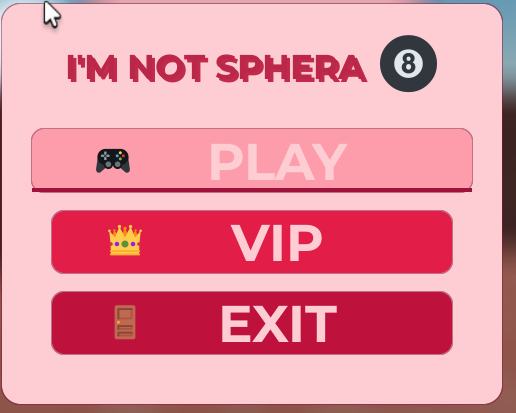
\includegraphics[width=\linewidth]{desarrollo/s1.png}
        \caption*{\textbf{Main Menu}}
    \end{minipage}
    \hfill
    \begin{minipage}[b]{0.32\textwidth}
        \centering
        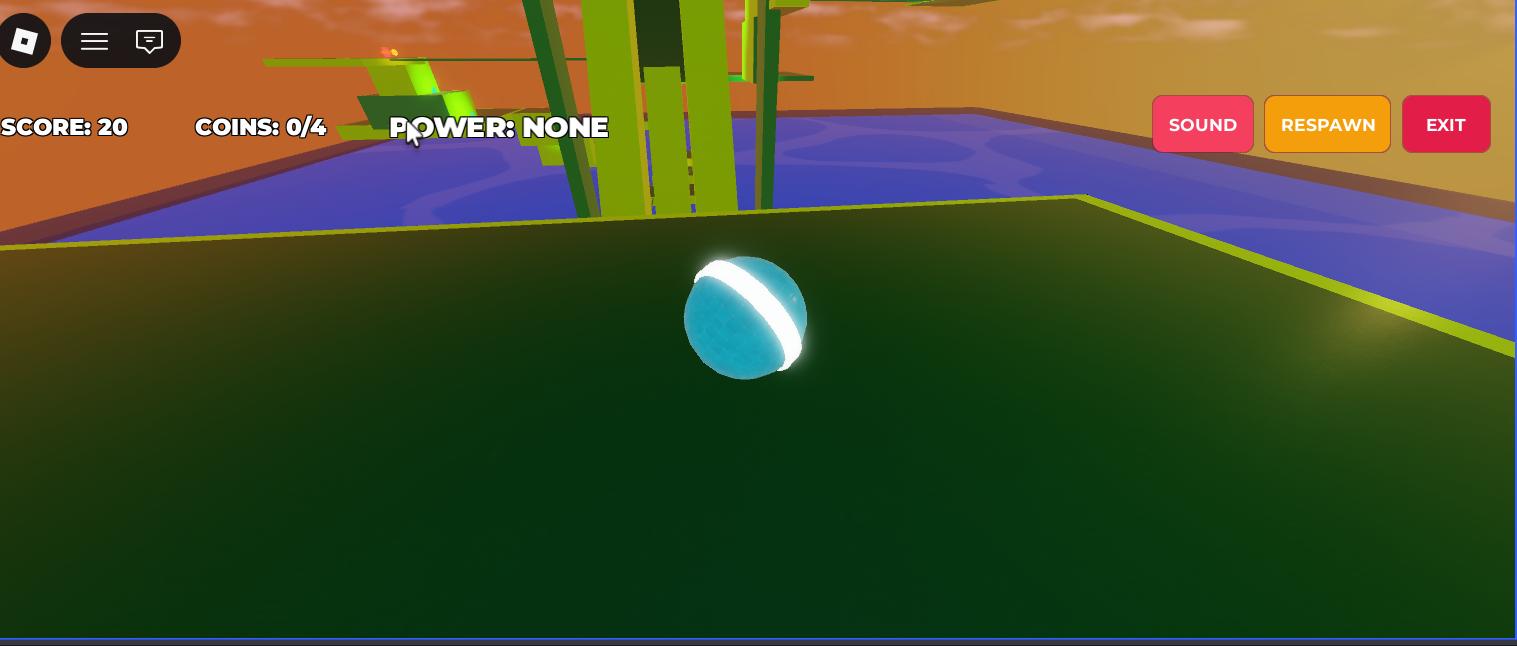
\includegraphics[width=\linewidth]{desarrollo/s2.png}
        \caption*{\textbf{Gameplay}}
    \end{minipage}
    \hfill
    \begin{minipage}[b]{0.32\textwidth}
        \centering
        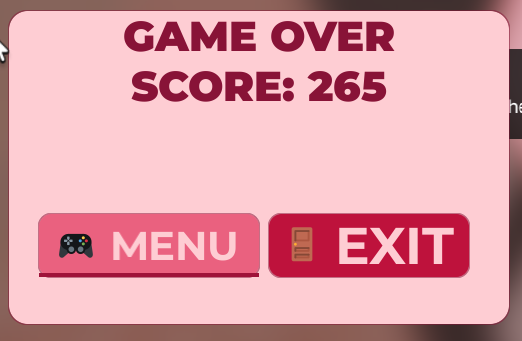
\includegraphics[width=\linewidth]{desarrollo/s3.png}
        \caption*{\textbf{Score Menu}}
    \end{minipage}
\end{figure}

\begin{figure}[H]
    \centering
    \begin{minipage}[b]{0.47\textwidth}
        \centering
        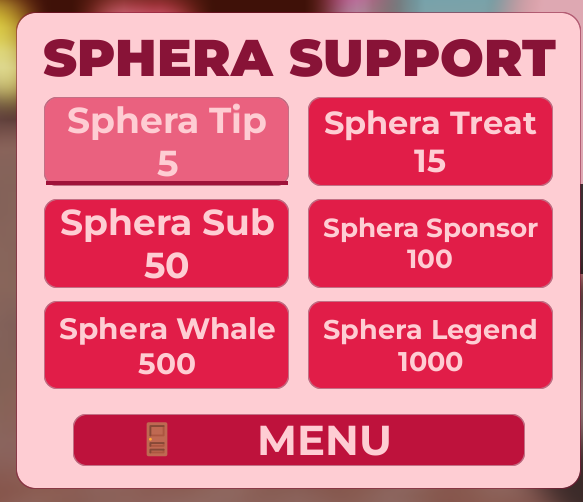
\includegraphics[width=\linewidth]{desarrollo/s4.png}
        \caption*{\textbf{VIP Menu}}
    \end{minipage}
    \hfill
    \begin{minipage}[b]{0.47\textwidth}
        \centering
        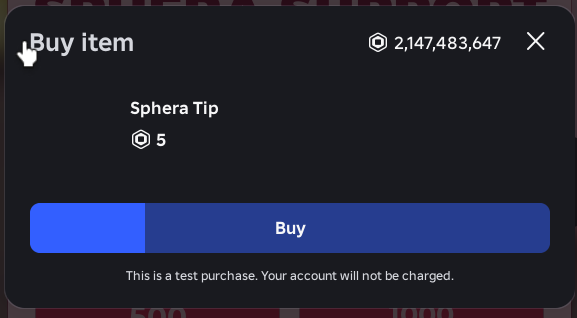
\includegraphics[width=\linewidth]{desarrollo/s5.png}
        \caption*{\textbf{Donation Interface}}
    \end{minipage}
\end{figure}

\begin{figure}[H]
    \centering
    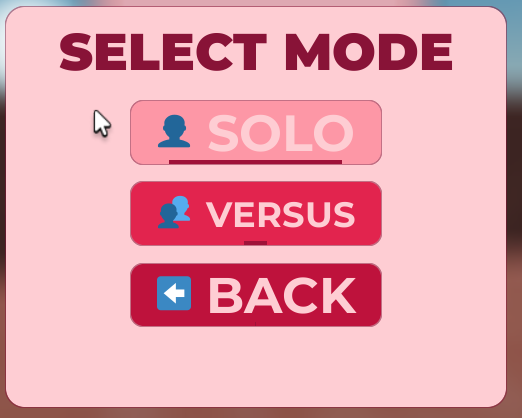
\includegraphics[width=0.6\textwidth]{desarrollo/s6.png}
    \caption*{\textbf{Global Score Table}}
\end{figure}

\begin{figure}[H]
    \centering
    \begin{minipage}[b]{0.32\textwidth}
        \centering
        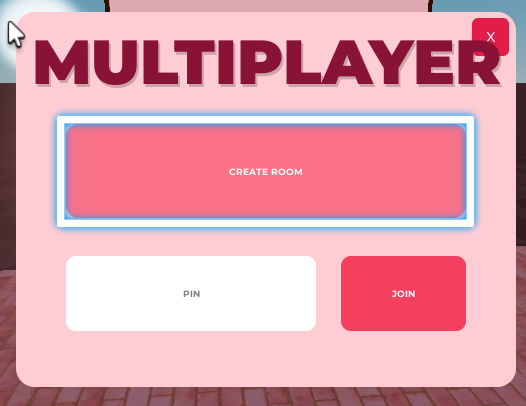
\includegraphics[width=\linewidth]{desarrollo/s7.png}
    \end{minipage}
    \hfill
    \begin{minipage}[b]{0.32\textwidth}
        \centering
        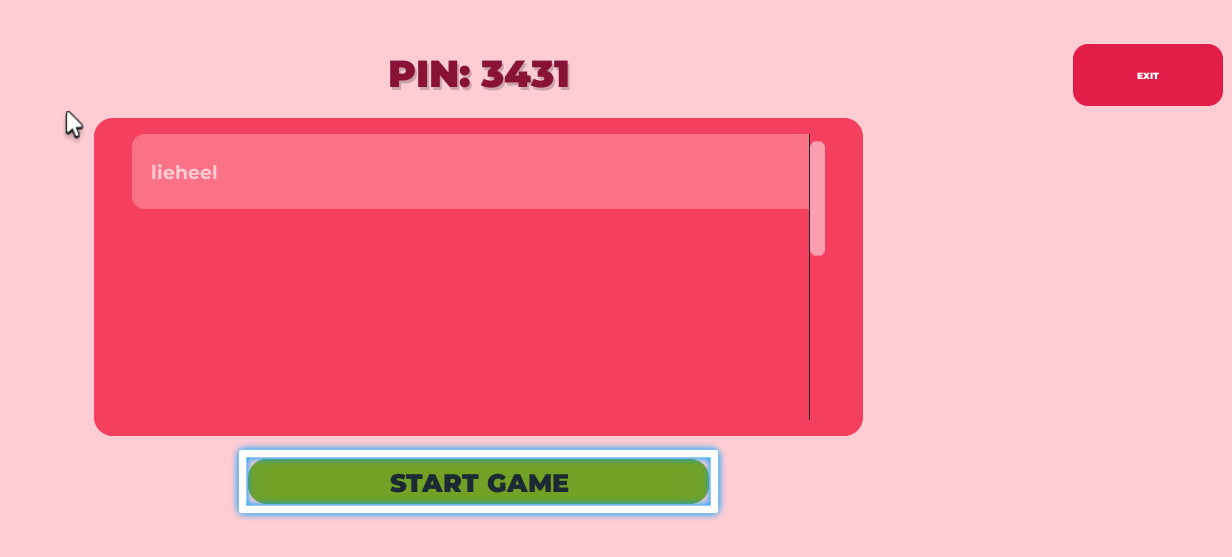
\includegraphics[width=\linewidth]{desarrollo/s8.png}
    \end{minipage}
    \hfill
    \begin{minipage}[b]{0.32\textwidth}
        \centering
        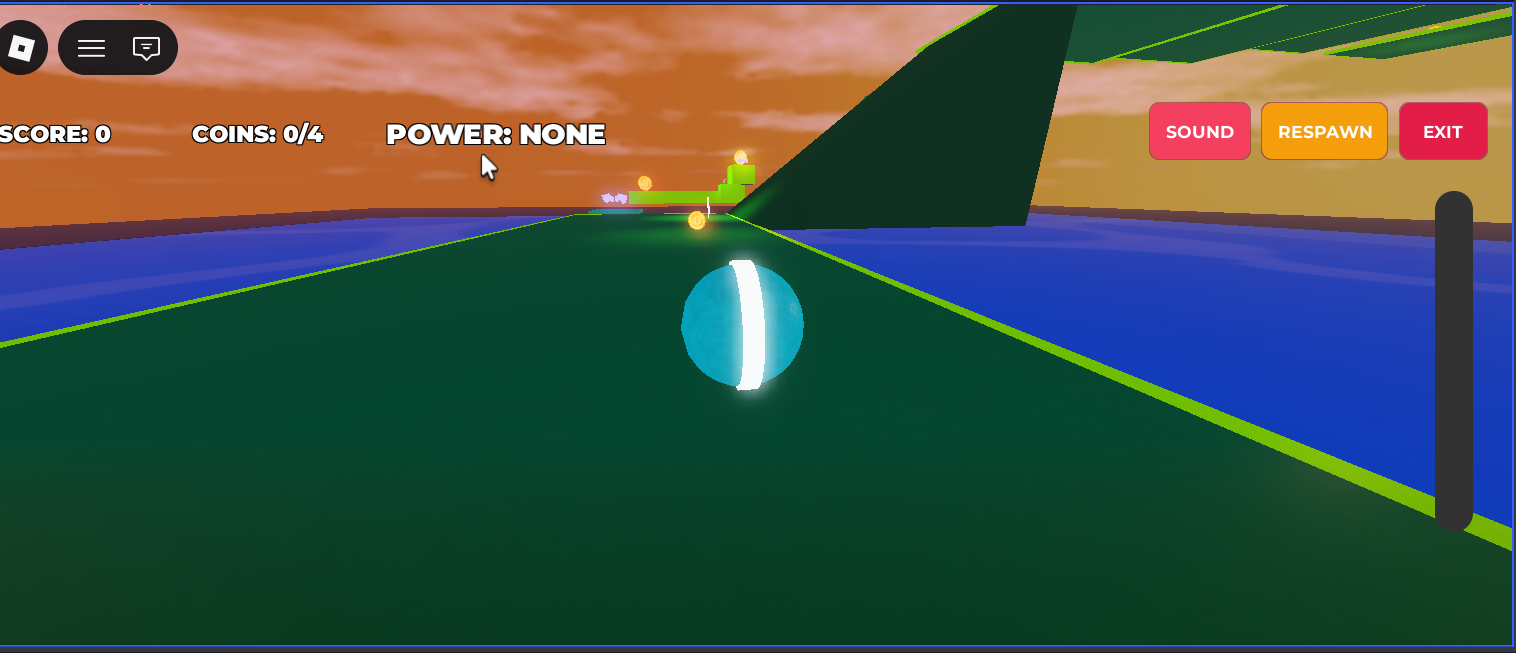
\includegraphics[width=\linewidth]{desarrollo/s9.png}
    \end{minipage}
    \caption{Multiplayer Lobby System: PIN entry, room creation, and versus mode.}
\end{figure}

\clearpage




\section{Shared Systems}

The arcade has ten games in total. Instead of writing the same interface, input, and leaderboard code again inside each one, three systems are shared across all of them: the score table system (the leaderboards), the menu system (the main menu, the VIP screen, and the game over screen), and the universal controller (the input that works on every device). This section explains how each shared system is built and which games use it.

\subsection{Score Table System}

All ten games report scores to a persistent leaderboard, so every game has an online ranking. There are two mechanisms, and which one a game uses depends on its complexity:

\begin{itemize}
  \item \textbf{Universal leaderboard} (seven games): Oxybelis, Avis Toucan, Resilio, Foxy Fruit, Firmament Defender, Firmament Siege, and Juice Cutter all report to the shared \texttt{UniversalLeaderboardModule}, which renders a single dynamic board (\texttt{UniversalLeaderboardClient}) that switches its title, icon, and color palette per game.
  \item \textbf{Dedicated score table} (three games): Turris Casei, Tap And Hold, and ImNotASphere each have their own in world board with a game specific leaderboard module and client. These three were given dedicated tables because they are the multiplayer games and need a board that lives permanently in their own arcade area.
\end{itemize}

Every board, universal or dedicated, is rendered as a physical part in the Workspace and updated in real time whenever any player finishes a session. The rest of this subsection describes the dedicated score table architecture; the universal leaderboard follows the same data flow pattern with a single shared module instead of one per game.

The state diagram below shows the idea: every board runs the very same code, and its \texttt{GameId} attribute is what decides which game it represents.

\begin{figure}[H]
  \centering
  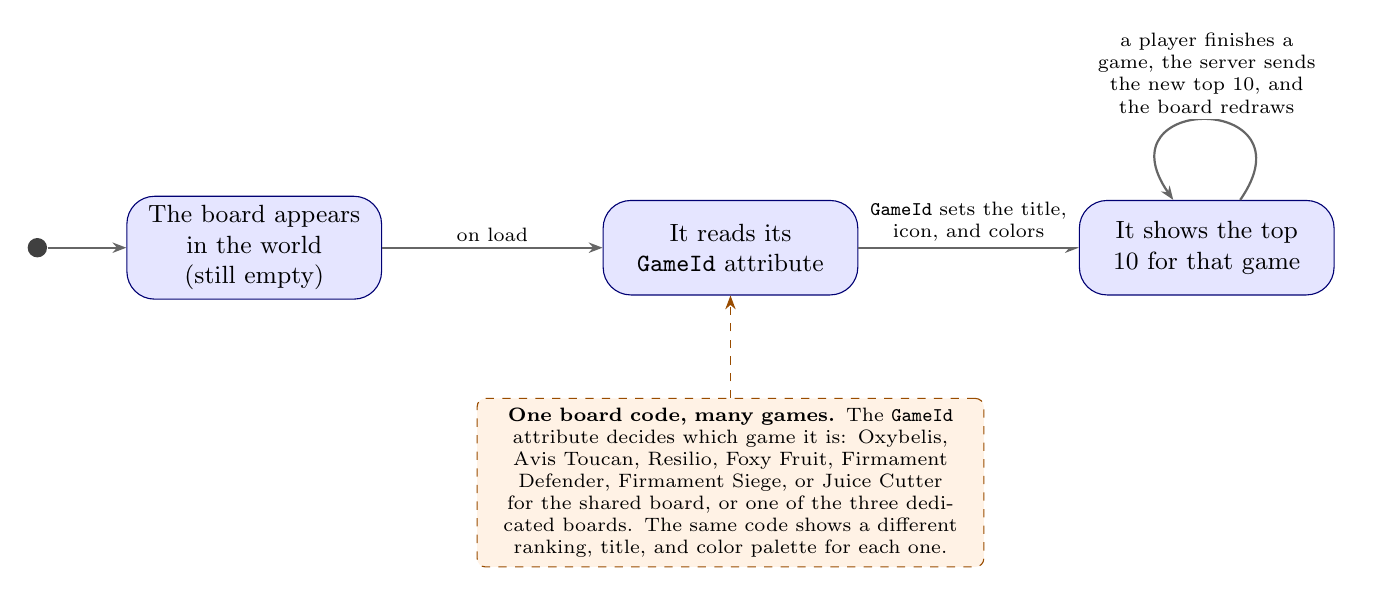
\begin{tikzpicture}[
  font=\small,
  >={Stealth[length=5pt]},
  state/.style={rectangle, rounded corners=10pt, draw=blue!45!black, fill=blue!10,
                text width=3cm, align=center, minimum height=1.2cm, font=\small},
  ini/.style={circle, fill=black!75, minimum size=7pt, inner sep=0},
  note/.style={rectangle, rounded corners=3pt, draw=orange!60!black, fill=orange!10, dashed,
               text width=6.2cm, align=center, font=\scriptsize},
  tr/.style={->, thick, draw=black!60},
  trlbl/.style={font=\scriptsize, fill=white, inner sep=2pt, align=center},
]

\node[ini] (i) {};
\node[state, right=1.0cm of i]  (s1) {The board appears in the world (still empty)};
\node[state, right=2.8cm of s1] (s2) {It reads its \texttt{GameId} attribute};
\node[state, right=2.8cm of s2] (s3) {It shows the top 10 for that game};

\draw[tr] (i) -- (s1);
\draw[tr] (s1) -- node[trlbl, above]{on load} (s2);
\draw[tr] (s2) -- node[trlbl, above, text width=2.6cm]{\texttt{GameId} sets the title, icon, and colors} (s3);
\draw[tr] (s3) to[out=55, in=125, looseness=5]
  node[trlbl, above, text width=3.4cm]{a player finishes a game, the server sends the new top 10, and the board redraws} (s3);

\node[note, below=1.3cm of s2] (n)
  {\textbf{One board code, many games.} The \texttt{GameId} attribute decides which game it is: Oxybelis, Avis Toucan, Resilio, Foxy Fruit, Firmament Defender, Firmament Siege, or Juice Cutter for the shared board, or one of the three dedicated boards. The same code shows a different ranking, title, and color palette for each one.};
\draw[dashed, draw=orange!60!black, ->] (n.north) -- (s2.south);

\end{tikzpicture}

  \caption{State diagram of a score table board. One code base behaves as any game's leaderboard depending on its \texttt{GameId} attribute.}
  \label{fig:scoretable_states}
\end{figure}

\subsubsection{Architecture}

Both mechanisms share the same three part architecture: a physical board in the Workspace, a module that handles DataStore persistence and ranking, and a client that renders the board. The only difference is whether these parts are game specific (dedicated) or shared across games (universal).

\begin{itemize}
  \item \textbf{Workspace Board} (Part): the physical leaderboard that players see in the arcade. Dedicated games use a named part (e.g.\ \texttt{TurrisCaseiLeaderboardPart}); universal games use a tagged \texttt{UniversalLeaderboardPart} carrying a \texttt{GAMEID} attribute that tells the shared client which game's scores to show.
  \item \textbf{Leaderboard Module} (ModuleScript in ReplicatedStorage/Modules): contains the DataStore read/write logic and the sorting algorithm that maintains the top ranking. It is required by the server and called after every game over event. Dedicated games have their own module; universal games all share \texttt{UniversalLeaderboardModule}.
  \item \textbf{Leaderboard Client} (LocalScript in StarterPlayerScripts): listens for the \texttt{Update...Leaderboard} RemoteEvent and rebuilds the board UI whenever new data arrives. Dedicated games have their own client; universal games all share \texttt{UniversalLeaderboardClient}.
\end{itemize}

\textbf{Dedicated architecture} (example: Turris Casei):
\begin{lstlisting}
|-- Workspace/
|   +-- TurrisCaseiLeaderboardPart     (named Score Table board)
|-- ReplicatedStorage/
|   |-- ArcadeRemotes/
|   |   +-- TurrisCasei/
|   |       +-- UpdateTurrisCaseiLeaderboard  (RemoteEvent)
|   +-- Modules/
|       +-- TurrisCaseiLeaderboard     (ModuleScript: DataStore + ranking)
+-- StarterPlayer/
    +-- StarterPlayerScripts/
        +-- TurrisCaseiLeaderboardClient (LocalScript: UI renderer)
\end{lstlisting}

\textbf{Universal architecture} (shared by the other seven games):
\begin{lstlisting}
|-- Workspace/
|   |-- UniversalLeaderboardPart (Tag="LeadboradOxybelis", GAMEID="Oxybelis")
|   |-- UniversalLeaderboardPart (Tag="LeadboradResilio",  GAMEID="Resilio")
|   +-- ... one tagged part per universal game ...
|-- ReplicatedStorage/
|   |-- ArcadeRemotes/
|   |   +-- GlobalBoard/
|   |       +-- UpdateUniversalLeaderboard  (RemoteEvent, shared)
|   +-- Modules/
|       +-- UniversalLeaderboardModule  (ModuleScript: shared DataStore + ranking)
+-- StarterPlayer/
    +-- StarterPlayerScripts/
        +-- UniversalLeaderboardClient  (LocalScript: shared renderer)
\end{lstlisting}

\subsubsection{Data Flow}

\begin{enumerate}
  \item A player finishes a session and the server calls the leaderboard module to report the score.
  \item The module reads the current top-10 from DataStore, inserts the new score if it qualifies, sorts by score descending (ties broken by time ascending), and writes the updated list back.
  \item The server fires \texttt{UpdateLeaderboard} to all clients with the new top-10 payload.
  \item Each leaderboard client receives the event and redraws the physical board in the Workspace.
\end{enumerate}

\subsubsection{Games Using This System}

All ten games are listed below with the mechanism each uses. The seven universal games share a single module and client, distinguished only by their \texttt{GAMEID}; the three dedicated games each have their own module and client.

\begin{table}[H]
\centering
\footnotesize
\begin{tabular}{|p{2.7cm}|p{2cm}|p{4.3cm}|p{4cm}|}
\hline
\textbf{Game} & \textbf{Mechanism} & \textbf{RemoteEvent} & \textbf{Leaderboard Module} \\
\hline
Oxybelis & Universal & UpdateUniversalLeaderboard & UniversalLeaderboardModule \\
\hline
Avis Toucan & Universal & UpdateUniversalLeaderboard & UniversalLeaderboardModule \\
\hline
Resilio & Universal & UpdateUniversalLeaderboard & UniversalLeaderboardModule \\
\hline
Foxy Fruit & Universal & UpdateUniversalLeaderboard & UniversalLeaderboardModule \\
\hline
Firmament Defender & Universal & UpdateUniversalLeaderboard & UniversalLeaderboardModule \\
\hline
Firmament Siege & Universal & UpdateUniversalLeaderboard & UniversalLeaderboardModule \\
\hline
Juice Cutter & Universal & UpdateUniversalLeaderboard & UniversalLeaderboardModule \\
\hline
Turris Casei & Dedicated & UpdateTurrisCaseiLeaderboard & TurrisCaseiLeaderboard \\
\hline
Tap And Hold & Dedicated & UpdateTapAndHoldLeaderboard & TapAndHoldLeaderboard \\
\hline
ImNotASphere & Dedicated & UpdateImNotASphereLeaderboard & ImNotASphereLeaderboard \\
\hline
\end{tabular}
\caption{Leaderboard mechanism for all ten games.}
\end{table}

\clearpage

\subsection{Menu System}

Every game opens the same style of menu: a main screen with PLAY, VIP, and EXIT buttons, a VIP donation screen, and a game over screen. Rather than rebuild this for each game, the menus are centralized into two shared modules in \texttt{ReplicatedStorage/Menu}. The split exists because the first seven games are single player and need only a simple menu, while the last three add a multiplayer lobby that requires a much larger menu module.

\begin{lstlisting}
ReplicatedStorage/
+-- Menu/ (Folder)
    |-- Menu1to7   (ModuleScript: single player menus, games 1-7)
    +-- Menu8to10  (ModuleScript: menus + multiplayer lobby, games 8-10)
\end{lstlisting}

The table below shows exactly which game uses which menu module:

\begin{table}[H]
\centering
\begin{tabular}{|p{3.5cm}|p{6.5cm}|p{4cm}|}
\hline
\textbf{Menu Module} & \textbf{Games} & \textbf{Type} \\
\hline
Menu1to7 & Oxybelis, Avis Toucan, Resilio, Foxy Fruit, Firmament Defender, Firmament Siege, Juice Cutter & Single player menus \\
\hline
Menu8to10 & Turris Casei, Tap And Hold, ImNotASphere & Menus + multiplayer lobby \\
\hline
\end{tabular}
\caption{Menu module assignment per game.}
\end{table}

The state diagram below shows how a player moves between the menu screens. The Lobby states only exist for the three multiplayer games that use \texttt{Menu8to10}; the other seven use \texttt{Menu1to7} and never enter the Lobby.

\begin{figure}[H]
  \centering
  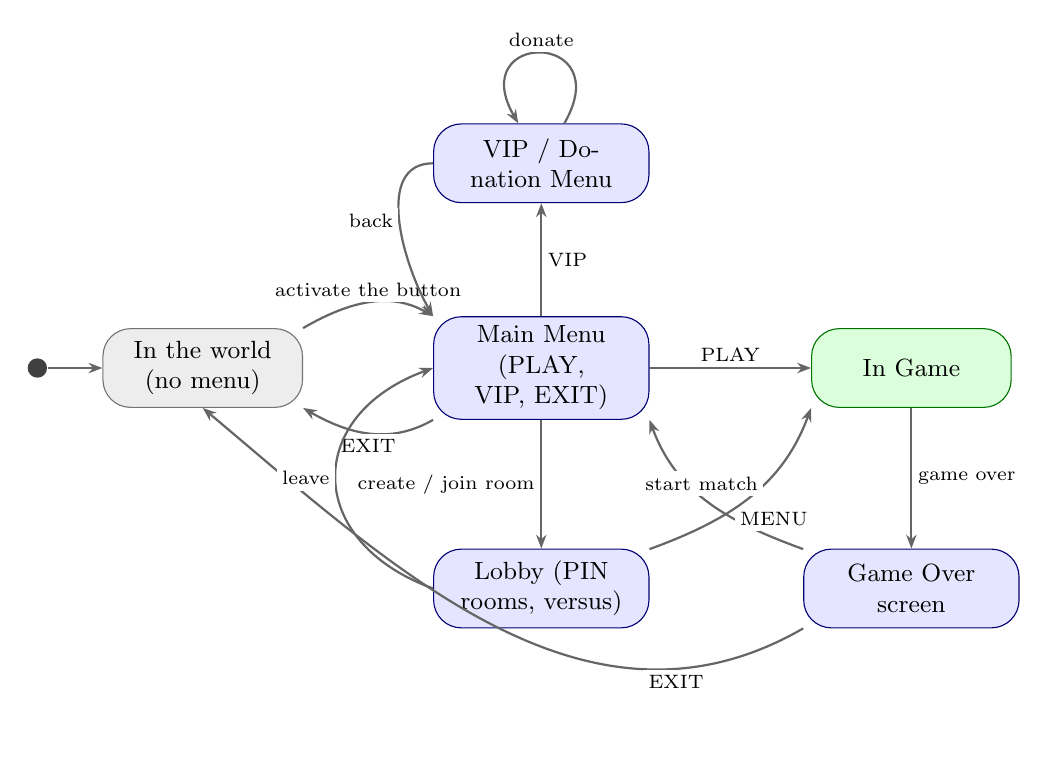
\begin{tikzpicture}[
  font=\small,
  >={Stealth[length=5pt]},
  state/.style={rectangle, rounded corners=10pt, draw=blue!45!black, fill=blue!10,
                text width=2.5cm, align=center, minimum height=1.0cm, font=\small},
  game/.style={rectangle, rounded corners=10pt, draw=green!45!black, fill=green!14,
               text width=2.3cm, align=center, minimum height=1.0cm, font=\small},
  closed/.style={rectangle, rounded corners=10pt, draw=black!55, fill=black!7,
                 text width=2.3cm, align=center, minimum height=1.0cm, font=\small},
  ini/.style={circle, fill=black!75, minimum size=7pt, inner sep=0},
  tr/.style={->, thick, draw=black!60},
  trlbl/.style={font=\scriptsize, fill=white, inner sep=2pt, align=center},
]

\node[ini]    (i)      at (-2.1,0)  {};
\node[closed] (world)  at (0,0)     {In the world (no menu)};
\node[state]  (main)   at (4.3,0)   {Main Menu (PLAY, VIP, EXIT)};
\node[state]  (vip)    at (4.3,2.6) {VIP / Donation Menu};
\node[game]   (ingame) at (9.0,0)   {In Game};
\node[state]  (over)   at (9.0,-2.8){Game Over screen};
\node[state]  (lobby)  at (4.3,-2.8){Lobby (PIN rooms, versus)};

\draw[tr] (i) -- (world);
\draw[tr] (world.north east) to[out=30,in=150] node[trlbl, above]{activate the button} (main.north west);
\draw[tr] (main.south west) to[out=210,in=330] node[trlbl, below]{EXIT} (world.south east);

\draw[tr] (main) -- node[trlbl, right]{VIP} (vip);
\draw[tr] (vip.west) to[out=180,in=120] node[trlbl, left]{back} (main.north west);
\draw[tr] (vip) to[out=60,in=120,looseness=6] node[trlbl, above]{donate} (vip);

\draw[tr] (main) -- node[trlbl, above]{PLAY} (ingame);
\draw[tr] (ingame) -- node[trlbl, right]{game over} (over);
\draw[tr] (over) to[out=160,in=290] node[trlbl, pos=0.35, right]{MENU} (main.south east);

\draw[tr] (over.south west) to[out=210,in=320] node[trlbl, pos=0.2, below]{EXIT} (world.south);

\draw[tr] (main) -- node[trlbl, left]{create / join room} (lobby);
\draw[tr] (lobby) to[out=20,in=250] node[trlbl, pos=0.6, left]{start match} (ingame.south west);
\draw[tr] (lobby.west) to[out=160,in=200,looseness=1.6] node[trlbl, left]{leave} (main.west);

\end{tikzpicture}

  \caption{State diagram of the menu system. The Lobby states belong to \texttt{Menu8to10} (the three multiplayer games); \texttt{Menu1to7} skips them.}
  \label{fig:menu_states}
\end{figure}

\subsubsection{Menu1to7 (Single Player Menu)}

\texttt{Menu1to7} drives the menus for the seven single player games: Oxybelis, Avis Toucan, Resilio, Foxy Fruit, Firmament Defender, Firmament Siege, and Juice Cutter. Each game passes a configuration table describing its title, icon, color palette, and donation products, and the module builds the UI from that data. This is why all seven games share an identical menu layout but each has its own colors and branding.

The module exposes four public functions:
\begin{itemize}
  \item \texttt{AbrirMenuPrincipal(config)} builds the main menu with the PLAY, VIP, and EXIT buttons from the config that was passed in.
  \item \texttt{AbrirMenuVIP()} builds the donation grid, with one button for each product in the config.
  \item \texttt{AbrirGameOver(score, perfect)} shows the final score with the MENU and EXIT options.
  \item \texttt{CerrarMenu()} closes all the menu screens and gives the camera and the player controls back.
\end{itemize}

Beyond layout, the module handles focus management (\texttt{EstablecerEnfoque}): it applies a blur effect, freezes the camera, disables the default character controller, and turns off proximity prompts while a menu is open. Keyboard and gamepad navigation is routed through the universal controller so the same up/down/confirm/back logic works on every platform.

\subsubsection{Menu8to10 (Menu + Multiplayer Lobby)}

\texttt{Menu8to10} drives the menus for the three multiplayer games: Turris Casei, Tap And Hold, and ImNotASphere. It includes everything \texttt{Menu1to7} does, plus a full lobby system: room creation with a PIN code, a screen to join a room by its PIN, a room player list with host kick controls, a button to start a versus match, and a spectator view. Instead of a config table passed per call, it exposes a \texttt{Config} table (title, color palettes for both menu and lobby, donation products) and a \texttt{Callbacks} table that the game's client script fills in with handlers like \texttt{OnCreateRoom}, \texttt{OnJoinRoom}, \texttt{OnStartMatch}, and \texttt{OnKickPlayer}.

The lobby uses a second color palette (\texttt{LobbyColors}) distinct from the main menu palette, so the lobby screens are visually separated from the game's branded menu.

\subsection{Universal Controller}

The universal controller (\texttt{UniversalController}, a ModuleScript in StarterPlayerScripts) is the single input layer shared by all ten games. Its job is to map one logical action set per game onto four different input methods: keyboard, mouse, gamepad, and on screen touch controls. Each game calls one bind function, and the controller wires up every platform at once. This is what makes the "adapted for mobile, Xbox, and PlayStation" claim true for every game without per platform code inside the games themselves.

The state diagram below shows how the controller switches its mode based on the last device the player used. The game actions stay the same; only the way they are read changes.

\begin{figure}[H]
  \centering
  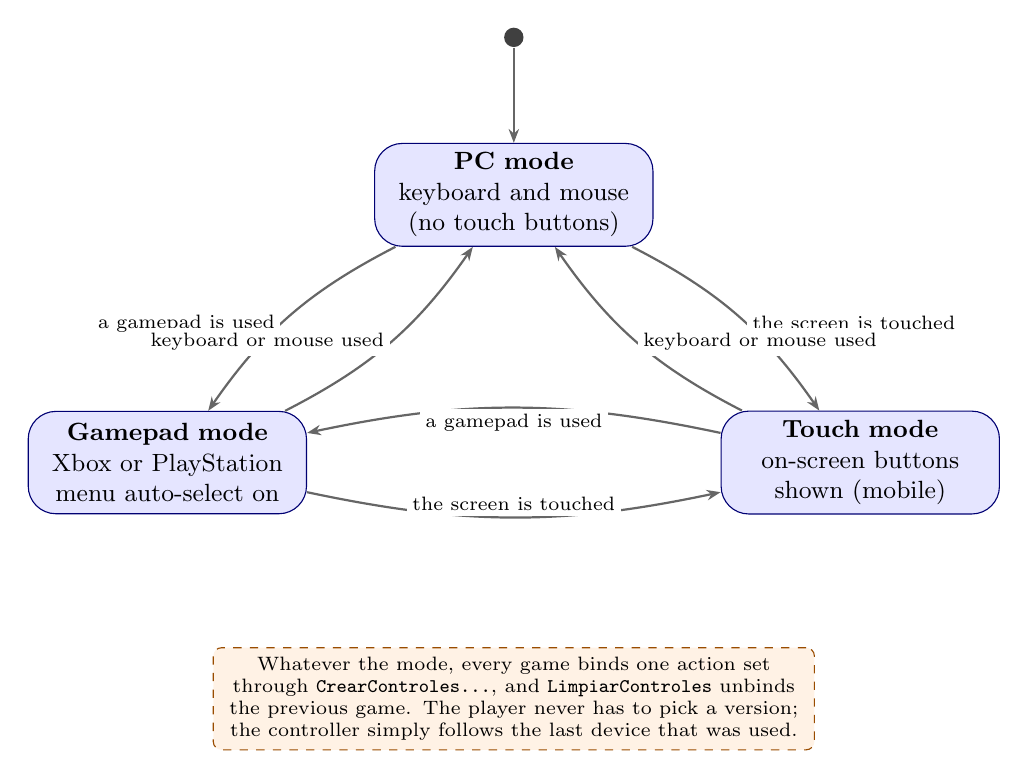
\begin{tikzpicture}[
  font=\small,
  >={Stealth[length=5pt]},
  state/.style={rectangle, rounded corners=10pt, draw=blue!45!black, fill=blue!10,
                text width=3.3cm, align=center, minimum height=1.3cm, font=\small},
  ini/.style={circle, fill=black!75, minimum size=7pt, inner sep=0},
  note/.style={rectangle, rounded corners=3pt, draw=orange!60!black, fill=orange!10, dashed,
               text width=7.4cm, align=center, font=\scriptsize},
  tr/.style={->, thick, draw=black!60},
  trlbl/.style={font=\scriptsize, fill=white, inner sep=2pt, align=center},
]

\node[state] (pc)    at (0,0)      {\textbf{PC mode}\\keyboard and mouse\\(no touch buttons)};
\node[state] (pad)   at (-4.4,-3.4){\textbf{Gamepad mode}\\Xbox or PlayStation\\menu auto-select on};
\node[state] (touch) at (4.4,-3.4) {\textbf{Touch mode}\\on-screen buttons\\shown (mobile)};
\node[ini]   (i)     at (0,2.0)    {};

\draw[tr] (i) -- (pc);

\draw[tr] (pc) to[bend right=14] node[trlbl, left, pos=0.55]{a gamepad is used} (pad);
\draw[tr] (pad) to[bend right=14] node[trlbl, left, pos=0.5]{keyboard or mouse used} (pc);

\draw[tr] (pc) to[bend left=14] node[trlbl, right, pos=0.55]{the screen is touched} (touch);
\draw[tr] (touch) to[bend left=14] node[trlbl, right, pos=0.5]{keyboard or mouse used} (pc);

\draw[tr] (pad) to[bend right=12] node[trlbl, above]{the screen is touched} (touch);
\draw[tr] (touch) to[bend right=12] node[trlbl, below]{a gamepad is used} (pad);

\node[note] (n) at (0,-6.4)
  {Whatever the mode, every game binds one action set through \texttt{CrearControles...}, and \texttt{LimpiarControles} unbinds the previous game. The player never has to pick a version; the controller simply follows the last device that was used.};

\end{tikzpicture}

  \caption{State diagram of the universal controller. It follows the last input device, switching between PC, gamepad, and touch.}
  \label{fig:controller_states}
\end{figure}

\subsubsection{Menu Navigation Helpers}

Three functions provide cross platform menu navigation, used by both menu modules:
\begin{itemize}
  \item \texttt{EsBotonSeleccion(input)} is the confirm key: Enter, Space, or the A button on a gamepad.
  \item \texttt{EsBotonAtras(input)} is the cancel key: Escape or the B button on a gamepad.
  \item \texttt{ObtenerDireccionMenu(input)} turns WASD, the arrow keys, or the direction pad into a direction.
\end{itemize}

\subsubsection{Per Game Control Bindings}

Each game has a dedicated bind function that registers its keyboard and gamepad actions via \texttt{ContextActionService} and, on touch devices, spawns the matching on screen controls. When a new game starts, \texttt{LimpiarControles} unbinds the previous game's actions and destroys its virtual controls, so only one control set is ever active.

All bind functions share the \texttt{CrearControles} prefix (e.g.\ \texttt{CrearControlesOxybelis}); the table below lists each by its game specific suffix.

\begin{table}[H]
\centering
\footnotesize
\begin{tabular}{|p{3cm}|p{6cm}|p{4.5cm}|}
\hline
\textbf{Game (bind suffix)} & \textbf{Control Scheme} & \textbf{Touch UI} \\
\hline
Oxybelis & four direction direction pad & Dual cross pad \\
\hline
Flappy (Avis Toucan) & Single flap button & Tap buttons \\
\hline
Resilio & Left/right + launch & Cross pad variant \\
\hline
FoxyFruit & four direction direction pad & Dual cross pad \\
\hline
Firmament (Defender) & four direction + fire & Cross pad + fire button \\
\hline
FirmamentSiege & Twin stick + fire & Dual joystick + fire \\
\hline
JuiceCutter & Joystick + cut & Gamepad / touch swipe \\
\hline
Turris (Casei) & Single drop button & Drop button \\
\hline
TapAndHold & Hold / release button & Hold jump button \\
\hline
ImNotASphere & Twin stick + jump + power & Dual joystick + 2 buttons \\
\hline
\end{tabular}
\caption{Per game control bindings in the Universal Controller (function = \texttt{CrearControles} + suffix).}
\end{table}

\subsubsection{Virtual Control Widgets}

For touch devices, the controller builds the on screen UI from a small set of reusable widgets, all sharing one neon visual style: a four direction cross pad, a circular action button, a draggable analog joystick (with normalized vector output), and a Resilio specific cross pad with a wide launch button. A connection to \texttt{LastInputTypeChanged} automatically hides the touch controls and enables gamepad GUI navigation when a controller is detected, and shows them again on touch input.

\subsection{Multiplayer Lobby System}

Three of the ten games support multiplayer: Turris Casei, Tap And Hold, and ImNotASphere. They all share the exact same lobby system, so it is documented once here rather than three times. On the server it is driven by a match manager, and on the client by a fixed set of RemoteEvents and RemoteFunctions (\texttt{CreateRoom}, \texttt{JoinRoom}, \texttt{StartMultiplayerMatch}, \texttt{RoomUpdate}, \texttt{UpdateLiveScore}, \texttt{PlayerDied}, \texttt{SpectateTarget}, \texttt{KickPlayer}, and \texttt{LeaveRoom}).

Rooms are private and protected by a four digit PIN. There are no public lobbies and no random matchmaking: a player can only join a room if someone shares the PIN with them outside the game, through a chat or a message. This is a deliberate safety choice for a young audience, not a technical limit, and the host can remove any player from the room at any time.

The sequence diagram below follows the whole flow over time, between the host, a guest, and the server, from creating a room to announcing the winner. The arrows that go to both players (with a dot on the guest's lifeline) are the broadcasts that the server sends to everyone in the room.

\begin{figure}[H]
  \centering
  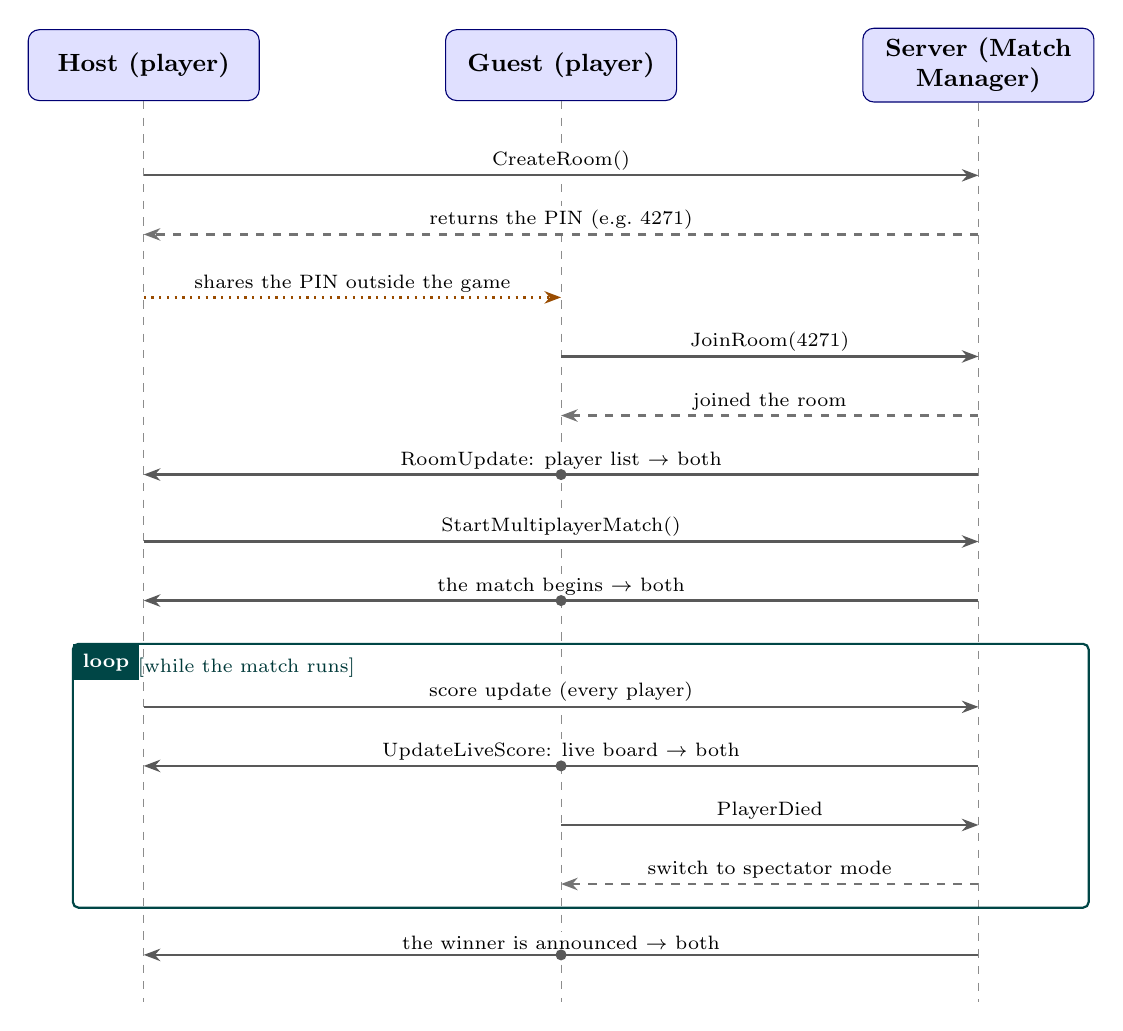
\begin{tikzpicture}[
  font=\small,
  >={Stealth[length=6pt]},
  party/.style={rectangle, rounded corners=4pt, draw=blue!45!black, fill=blue!12,
                align=center, font=\small\bfseries, minimum height=0.9cm, text width=2.7cm},
  life/.style={draw=black!45, dashed},
  msg/.style={->, thick, draw=black!65},
  ret/.style={->, thick, draw=black!55, dashed},
  ext/.style={->, thick, draw=orange!60!black, dotted},
  ml/.style={font=\scriptsize, fill=white, inner sep=1.5pt, align=center},
  dot/.style={circle, fill=black!65, minimum size=4pt, inner sep=0},
]

\def\hx{0}   \def\gx{5.3}  \def\sx{10.6}
\def\bot{-11.9}

% participants
\node[party] (host)   at (\hx,0) {Host (player)};
\node[party] (guest)  at (\gx,0) {Guest (player)};
\node[party] (server) at (\sx,0) {Server (Match Manager)};

% lifelines
\draw[life] (host.south)   -- (\hx,\bot);
\draw[life] (guest.south)  -- (\gx,\bot);
\draw[life] (server.south) -- (\sx,\bot);

% messages
\draw[msg] (\hx,-1.4) -- node[ml, above]{CreateRoom()} (\sx,-1.4);
\draw[ret] (\sx,-2.15) -- node[ml, above]{returns the PIN (e.g.\ 4271)} (\hx,-2.15);
\draw[ext] (\hx,-2.95) -- node[ml, above]{shares the PIN outside the game} (\gx,-2.95);
\draw[msg] (\gx,-3.7) -- node[ml, above]{JoinRoom(4271)} (\sx,-3.7);
\draw[ret] (\sx,-4.45) -- node[ml, above]{joined the room} (\gx,-4.45);

% broadcast: room update
\draw[msg] (\sx,-5.2) -- node[ml, above]{RoomUpdate: player list $\rightarrow$ both} (\hx,-5.2);
\node[dot] at (\gx,-5.2) {};

\draw[msg] (\hx,-6.05) -- node[ml, above]{StartMultiplayerMatch()} (\sx,-6.05);

% broadcast: match begins
\draw[msg] (\sx,-6.8) -- node[ml, above]{the match begins $\rightarrow$ both} (\hx,-6.8);
\node[dot] at (\gx,-6.8) {};

% loop frame
\draw[draw=teal!55!black, thick, rounded corners=2pt] (\hx-0.9,-7.35) rectangle (\sx+1.4,-10.7);
\node[fill=teal!55!black, text=white, font=\scriptsize\bfseries, anchor=north west]
  at (\hx-0.9,-7.35) {loop};
\node[font=\scriptsize, anchor=north west, text=teal!45!black] at (\hx-0.2,-7.4) {[while the match runs]};

\draw[msg] (\hx,-8.15) -- node[ml, above]{score update (every player)} (\sx,-8.15);
\draw[msg] (\sx,-8.9) -- node[ml, above]{UpdateLiveScore: live board $\rightarrow$ both} (\hx,-8.9);
\node[dot] at (\gx,-8.9) {};
\draw[msg] (\gx,-9.65) -- node[ml, above]{PlayerDied} (\sx,-9.65);
\draw[ret] (\sx,-10.4) -- node[ml, above]{switch to spectator mode} (\gx,-10.4);

% broadcast: winner
\draw[msg] (\sx,-11.3) -- node[ml, above]{the winner is announced $\rightarrow$ both} (\hx,-11.3);
\node[dot] at (\gx,-11.3) {};

\end{tikzpicture}

  \caption{Sequence diagram of a private multiplayer match, from creating the PIN room to the final winner.}
  \label{fig:sequence_multiplayer}
\end{figure}

\clearpage



\section{In Game Data Analytics System}

On top of the games themselves, the project includes a full data analytics system that tracks how each game is played and how much money it brings in. All of this data is shown on about fifteen physical boards inside a bank themed building in the game world, turning plain DataStore numbers into clear, live dashboards that any player can walk up to and read. The boards cover the stats for each game, overviews across all the games, the revenue, and live tickers of the most recent scores and donations.

The data flow diagram below shows the whole path: from a player finishing a game or making a donation, through the module that stores and aggregates the data, to the server that serves it, and finally to the boards the player reads.

\begin{figure}[H]
  \centering
  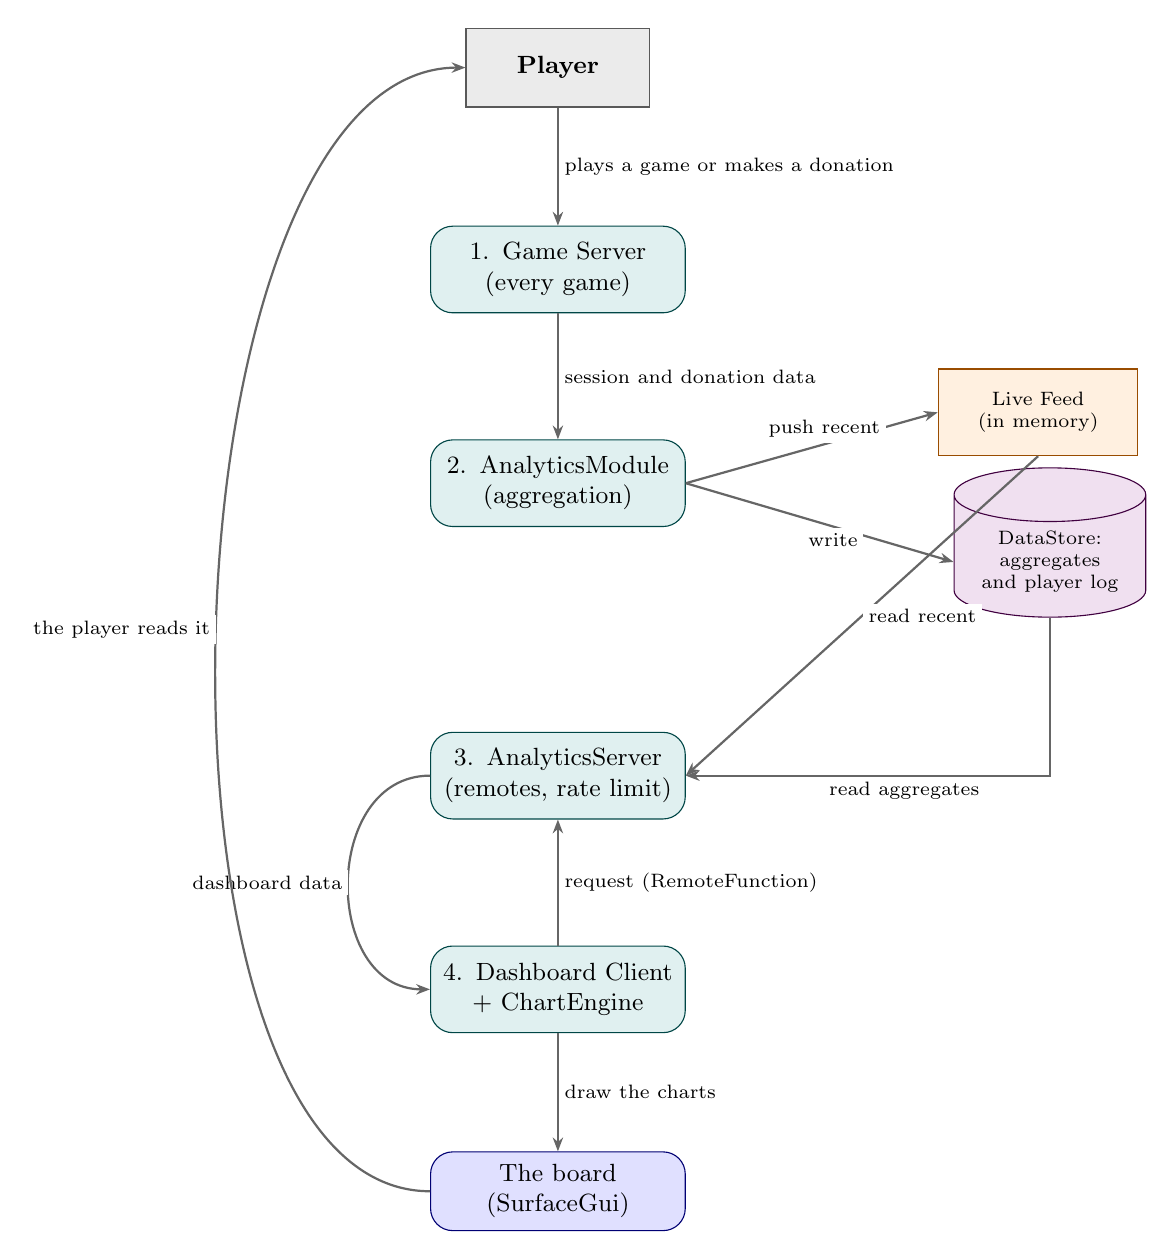
\begin{tikzpicture}[
  font=\small,
  >={Stealth[length=5pt]},
  entity/.style={rectangle, draw=black!65, fill=black!8, text width=2.1cm, align=center,
                 minimum height=1.0cm, font=\small\bfseries},
  proc/.style={rectangle, rounded corners=8pt, draw=teal!55!black, fill=teal!12,
               text width=3.0cm, align=center, minimum height=1.1cm, font=\small},
  store/.style={cylinder, shape border rotate=90, aspect=0.28, draw=violet!50!black,
                fill=violet!12, text width=2.2cm, align=center, minimum height=1.7cm,
                minimum width=1.5cm, font=\scriptsize},
  feed/.style={rectangle, draw=orange!60!black, fill=orange!12, text width=2.3cm,
               align=center, minimum height=1.1cm, font=\scriptsize},
  board/.style={rectangle, rounded corners=8pt, draw=blue!45!black, fill=blue!12,
                text width=3.0cm, align=center, minimum height=1.0cm, font=\small},
  flow/.style={->, thick, draw=black!60},
  fl/.style={font=\scriptsize, fill=white, inner sep=2pt, align=center},
]

\node[entity] (player) {Player};
\node[proc, below=1.5cm of player]   (gs)   {1. Game Server (every game)};
\node[proc, below=1.6cm of gs]       (am)   {2. AnalyticsModule (aggregation)};
\node[proc, below=2.6cm of am]       (as)   {3. AnalyticsServer (remotes, rate limit)};
\node[proc, below=1.6cm of as]       (dash) {4. Dashboard Client + ChartEngine};
\node[board, below=1.5cm of dash]    (board){The board (SurfaceGui)};

\node[feed,  right=3.2cm of am, yshift=0.9cm]  (feed) {Live Feed (in memory)};
\node[store, right=3.4cm of am, yshift=-1.0cm] (db)   {DataStore: aggregates and player log};

\draw[flow] (player) -- node[fl, right]{plays a game or makes a donation} (gs);
\draw[flow] (gs) -- node[fl, right]{session and donation data} (am);
\draw[flow] (am.east) -- node[fl, above, pos=0.55]{push recent} (feed.west);
\draw[flow] (am.east) -- node[fl, below, pos=0.55]{write} (db.west);
\draw[flow] (feed.south) -- node[fl, right]{read recent} (as.east);
\draw[flow] (db.south) |- node[fl, below, pos=0.7]{read aggregates} (as.east);
\draw[flow] (dash.north) -- node[fl, right]{request (RemoteFunction)} (as.south);
\draw[flow] (as.west) to[out=180, in=180, looseness=1.3] node[fl, left]{dashboard data} (dash.west);
\draw[flow] (dash) -- node[fl, right]{draw the charts} (board);
\draw[flow] (board.west) to[out=180, in=180, looseness=0.7] node[fl, left]{the player reads it} (player.west);

\end{tikzpicture}

  \caption{Data flow diagram of the analytics system, from gameplay to the boards on display.}
  \label{fig:analytics_dfd}
\end{figure}

\subsection{Architecture}

The analytics system is built from four components, following the same client and server separation as the games:

\begin{itemize}
  \item \textbf{AnalyticsModule} (ModuleScript in ReplicatedStorage/Modules): the data layer. It records finished sessions and donations, aggregates them into per game statistics, persists everything to DataStore, and builds the dashboard payloads consumed by the boards.
  \item \textbf{AnalyticsServer} (Script in ServerScriptService): the network layer. It exposes RemoteFunctions for each dashboard type, rate limits requests per player and per board, and broadcasts a periodic \texttt{DashboardUpdated} event so open boards refresh themselves.
  \item \textbf{ChartEngine} (ModuleScript in ReplicatedStorage/Modules): the rendering layer. It draws charts (bars, lines, histograms, donuts, and more) directly onto \texttt{EditableImage} canvases using a shared dark palette and per game brand colors.
  \item \textbf{AnalyticsDashboardClient} (LocalScript in StarterPlayerScripts): the display layer. It finds every part tagged \texttt{AnalyticsBoard} via \texttt{CollectionService}, reads its \texttt{GameId} attribute to decide which dashboard to render, and draws the board as a \texttt{SurfaceGui} on the physical part.
\end{itemize}

\begin{lstlisting}
Analytics System Structure
|-- Workspace/
|   +-- BankBuilding/ (themed building)
|       +-- ~15 Parts (Tag="AnalyticsBoard", Attribute GameId="...")
|-- ReplicatedStorage/
|   |-- AnalyticsRemotes/ (Folder)
|   |   |-- GetGameDashboard      (RemoteFunction)
|   |   |-- GetGeneralDashboard   (RemoteFunction)
|   |   |-- GetMoneyDashboard     (RemoteFunction)
|   |   |-- GetRecentDonations    (RemoteFunction)
|   |   |-- GetRecentScores       (RemoteFunction)
|   |   +-- DashboardUpdated      (RemoteEvent)
|   +-- Modules/
|       |-- AnalyticsModule       (ModuleScript: data + aggregation)
|       +-- ChartEngine           (ModuleScript: chart rendering)
|-- ServerScriptService/
|   +-- AnalyticsServer           (Script: remotes + rate limiting)
+-- StarterPlayer/
    +-- StarterPlayerScripts/
        +-- AnalyticsDashboardClient (LocalScript: board renderer)
\end{lstlisting}

\subsection{Data Collected Per Game}

Every game server already calls two one line helpers at the end of a run: \texttt{ReportSessionAsync} after each game over, and \texttt{ReportDonationAsync} inside its \texttt{ProcessReceipt} handler. These feed the analytics module, which maintains a per game aggregate in the \texttt{Analytics\_Aggregates\_v1} DataStore and a per player log in \texttt{Analytics\_PlayerLog\_v1}. From these, the system derives:

\begin{table}[H]
\centering
\footnotesize
\begin{tabular}{|p{4cm}|p{11.5cm}|}
\hline
\textbf{Category} & \textbf{Metrics} \\
\hline
Engagement & Total sessions, unique players, replay rate (sessions per player), average and total time played. \\
\hline
Scores & Average score, median score (estimated from a histogram of 20 buckets), max score seen, top 3 scores with player names. \\
\hline
Retention & Players grouped into 5 buckets by session count (1, 2 to 4, 5 to 9, 10 to 19, 20 or more). \\
\hline
Activity & Sessions by hour of day (24 buckets) and by weekday (7 buckets). \\
\hline
Revenue & Total donations (Robux), top 3 donors, revenue per hour and per weekday, revenue per player and per hour played. \\
\hline
Levels & Per level average completion time and max level reached (for games with levels). \\
\hline
Time Leaders & Top 3 players by cumulative time played. \\
\hline
Live Feeds & In memory ring buffers of the 40 most recent scores and donations across all games, newest first. \\
\hline
\end{tabular}
\caption{Data collected and derived per game by the analytics module.}
\end{table}

To keep DataStore reads low while many boards are open, aggregates are cached for 30 seconds, and writes use \texttt{UpdateAsync} so concurrent sessions never overwrite each other.

\subsection{Chart Engine}

The chart engine renders every visual directly onto an \texttt{EditableImage}, so the boards display real pixel drawn charts rather than stacked UI frames. It provides a reusable set of chart types, all themed with a dark palette and the same per game brand colors used elsewhere in the project:

\begin{table}[H]
\centering
\footnotesize
\begin{tabular}{|p{5cm}|p{10.5cm}|}
\hline
\textbf{Chart Type} & \textbf{Typical Use} \\
\hline
Vertical bar chart & Sessions or revenue compared across games. \\
\hline
Horizontal bar chart & Ranked comparisons (top scores, top donors). \\
\hline
Line chart & Activity or revenue trends across hours / weekdays. \\
\hline
Area chart & Filled trend lines for cumulative metrics. \\
\hline
Histogram & Score distribution across the 20 score buckets. \\
\hline
Scatter plot & Two variable comparisons (e.g.\ time vs.\ score). \\
\hline
Donut chart & Proportional breakdowns (retention buckets, revenue share). \\
\hline
Sparkline & Compact inline trend with no axes, used in summary tiles. \\
\hline
\end{tabular}
\caption{Chart types provided by the Chart Engine.}
\end{table}

\subsection{Board Types}

Each board is a tagged part whose \texttt{GameId} attribute selects which dashboard the client renders on it. There are three families of board: one dedicated dashboard per game, several cross game summary boards, and two live tickers.

\begin{table}[H]
\centering
\footnotesize
\begin{tabular}{|p{3.5cm}|p{12cm}|}
\hline
\textbf{Board (GameId)} & \textbf{Content} \\
\hline
Per game ($\times 10$) & One board per game (Oxybelis, Avis Toucan, Resilio, Foxy Fruit, Firmament Defender, Firmament Siege, Juice Cutter, Turris Casei, Tap And Hold, ImNotASphere) showing that game's full dashboard: engagement, scores, histogram, activity, and revenue. \\
\hline
General & Cross game overview: every game's headline numbers plus combined activity and retention. \\
\hline
Money & Revenue dashboard: donations per game, revenue per hour and per player. \\
\hline
MoneyG & Revenue focused chart variant of the money dashboard. \\
\hline
RealMoney & Live ticker of the most recent donations across all games (newest first). \\
\hline
RealPlayer & Live ticker of the most recent scores across all games (newest first). \\
\hline
LastMessage & Auxiliary board for the latest broadcast message. \\
\hline
\end{tabular}
\caption{The board types that make up the bank building (around fifteen boards in total).}
\end{table}

\subsection{Data Flow}

\begin{enumerate}
  \item A player finishes a game or makes a donation. The game server calls \texttt{ReportSessionAsync} or \texttt{ReportDonationAsync}.
  \item \texttt{AnalyticsModule} updates the per game aggregate and per player log in DataStore via \texttt{UpdateAsync}, and pushes the event onto the live feed ring buffers.
  \item A board exists in the world tagged \texttt{AnalyticsBoard}. On spawn, the client reads its \texttt{GameId}, renders an empty board immediately, then requests real data through the matching RemoteFunction.
  \item \texttt{AnalyticsServer} returns the dashboard payload (rate limited per player and per board).
  \item The client passes the payload to \texttt{ChartEngine}, which draws the charts onto an \texttt{EditableImage} shown on the board's \texttt{SurfaceGui}.
  \item Every 30 seconds the server fires \texttt{DashboardUpdated}; open boards refresh. The two live ticker boards poll every few seconds for a near real time feed.
\end{enumerate}

\section{Fireworks System}

Besides the ten arcade games, the island has a fireworks stand. A player walks up to it, opens a menu of nineteen fireworks and launches one into the sunset sky. Every other player in the server sees the same show at the same time, and the launcher additionally gets a short cinematic camera that chases the shell up and pulls back on the burst.

The system is deliberately split so that the server owns the rules and the client owns the spectacle: the server decides \emph{whether} a launch is allowed and broadcasts \emph{which} firework went off, while each client renders the whole thing locally. Nothing about the visual effect is replicated, which is what keeps a busy sky cheap, and it also means every player can independently choose not to see other people's fireworks.

\begin{figure}[H]
  \centering
  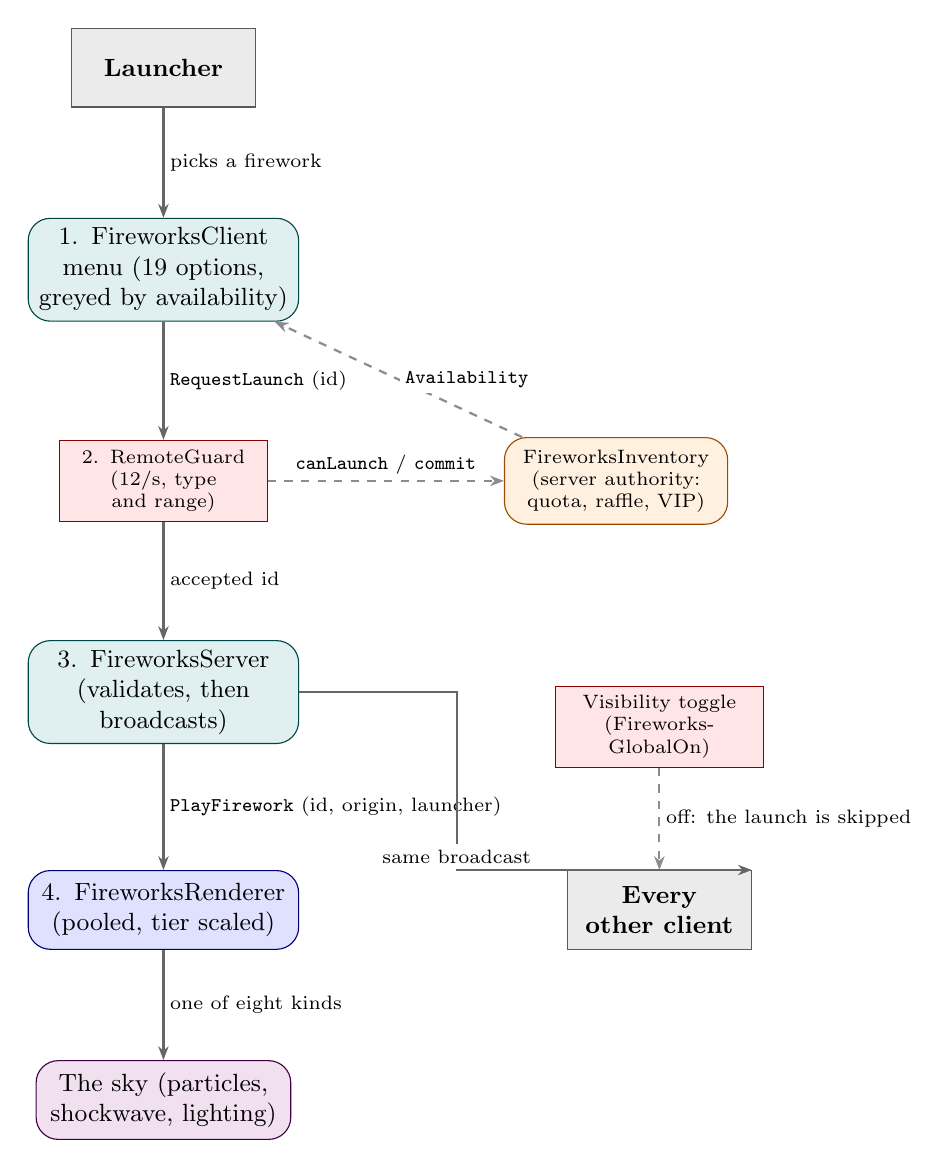
\begin{tikzpicture}[
  font=\small,
  >={Stealth[length=5pt]},
  entity/.style={rectangle, draw=black!65, fill=black!8, text width=2.1cm, align=center,
                 minimum height=1.0cm, font=\small\bfseries},
  proc/.style={rectangle, rounded corners=8pt, draw=teal!55!black, fill=teal!12,
               text width=3.2cm, align=center, minimum height=1.1cm, font=\small},
  econ/.style={rectangle, rounded corners=8pt, draw=orange!60!black, fill=orange!12,
               text width=2.6cm, align=center, minimum height=1.1cm, font=\scriptsize},
  guard/.style={rectangle, draw=red!55!black, fill=red!10, text width=2.4cm,
                align=center, minimum height=1.0cm, font=\scriptsize},
  render/.style={rectangle, rounded corners=8pt, draw=blue!45!black, fill=blue!12,
                 text width=3.2cm, align=center, minimum height=1.0cm, font=\small},
  sky/.style={rectangle, rounded corners=8pt, draw=violet!50!black, fill=violet!12,
              text width=3.0cm, align=center, minimum height=1.0cm, font=\small},
  flow/.style={->, thick, draw=black!60},
  side/.style={->, thick, draw=black!45, dashed},
  fl/.style={font=\scriptsize, fill=white, inner sep=2pt, align=center},
]

\node[entity] (player) {Launcher};
\node[proc,   below=1.4cm of player] (menu)  {1. FireworksClient menu (19 options, greyed by availability)};
\node[guard,  below=1.5cm of menu]   (rg)    {2. RemoteGuard (12/s, type and range)};
\node[econ,   right=3.0cm of rg]     (inv)   {FireworksInventory (server authority: quota, raffle, VIP)};
\node[proc,   below=1.5cm of rg]     (srv)   {3. FireworksServer (validates, then broadcasts)};
\node[render, below=1.6cm of srv]    (rend)  {4. FireworksRenderer (pooled, tier scaled)};
\node[sky,    below=1.4cm of rend]   (sky)   {The sky (particles, shockwave, lighting)};

\node[entity, right=3.4cm of rend]   (others) {Every other client};
\node[guard,  above=1.3cm of others] (toggle) {Visibility toggle (FireworksGlobalOn)};

\draw[flow] (player) -- node[fl, right]{picks a firework} (menu);
\draw[flow] (menu)   -- node[fl, right]{\texttt{RequestLaunch} (id)} (rg);
\draw[flow] (rg)     -- node[fl, right]{accepted id} (srv);
\draw[side] (rg)     -- node[fl, above]{\texttt{canLaunch} / \texttt{commit}} (inv);
\draw[side] (inv)    -- node[fl, right]{\texttt{Availability}} (menu);
\draw[flow] (srv)    -- node[fl, right]{\texttt{PlayFirework} (id, origin, launcher)} (rend);
\draw[flow] (rend)   -- node[fl, right]{one of eight kinds} (sky);

\draw[flow] (srv.east) -- ++(2.0,0) |- node[fl, above]{same broadcast} (others.north east);
\draw[side] (toggle)   -- node[fl, right]{off: the launch is skipped} (others);

\end{tikzpicture}

  \caption{Data flow of the fireworks system, from the launch request to the sky.}
  \label{fig:fireworks_dfd}
\end{figure}

\subsection{Architecture}

The system is made of five scripts plus a shared UI module, following the same client and server separation as the games:

\begin{itemize}
  \item \textbf{FireworksModule} (ModuleScript in ReplicatedStorage/Modules): the data layer. It holds the remote names, the VIP Game Pass id, the two timing constants, and the \texttt{Types} table: nineteen definitions that describe every firework purely as data (colours, apex height, particle speed, spread, lifetime, drag, gravity and a \texttt{kind} field).
  \item \textbf{FireworksInventory} (ModuleScript in ServerScriptService): the economy layer. It is the single authority on who may launch what. It tracks per player quotas, the free gift, the raffle, the time milestones and the VIP pass, and pushes a per type availability table back to each client so the menu can grey out what is not currently launchable.
  \item \textbf{FireworksServer} (Script in ServerScriptService): the network layer. It creates the remotes, wires the physical stand button, validates every request through \texttt{RemoteGuard} and, once a launch is accepted, broadcasts \texttt{PlayFirework} to all clients with the firework id, the world origin and the player who launched it.
  \item \textbf{FireworksClient} (LocalScript in StarterPlayerScripts): the interface layer. It builds the selection menu, handles keyboard and gamepad navigation, shows the toast notifications, drives the cinematic camera for the launcher, and decides whether an incoming broadcast should be rendered at all.
  \item \textbf{FireworksRenderer} (ModuleScript in StarterPlayerScripts): the rendering layer. It turns a firework id into particles. It pools every part it creates, scales particle counts by device tier, and caps how many shows may run at once.
  \item \textbf{ToggleButton} (ModuleScript in StarterPlayerScripts): the shared pill toggle used by the visibility button in the top right corner.
\end{itemize}

\begin{lstlisting}
Fireworks System Structure
|-- Workspace/
|   |-- FireworksButton        (Part: the stand the player activates)
|   +-- FireworkEffects/       (Folder: every pooled part lives here)
|-- ReplicatedStorage/
|   |-- FireworksRemotes/ (Folder)
|   |   |-- RequestLaunch      (RemoteEvent: client -> server, firework id)
|   |   |-- OpenMenu           (RemoteEvent: server -> client, open the menu)
|   |   |-- PlayFirework       (RemoteEvent: server -> all, id + origin + launcher)
|   |   |-- Notify             (RemoteEvent: server -> client, economy messages)
|   |   +-- Availability       (RemoteEvent: server -> client, per type greying)
|   +-- Modules/
|       +-- FireworksModule    (ModuleScript: the 19 definitions + constants)
|-- ServerScriptService/
|   |-- FireworksServer        (Script: remotes, validation, broadcast)
|   |-- FireworksInventory     (ModuleScript: quotas, raffle, VIP)
|   +-- RemoteGuard            (ModuleScript: rate limit + argument checks)
+-- StarterPlayer/
    +-- StarterPlayerScripts/
        |-- FireworksClient    (LocalScript: menu, toasts, cinematic camera)
        |-- FireworksRenderer  (ModuleScript: particle rendering)
        |-- FireworksToggle    (LocalScript: visibility button)
        +-- ToggleButton       (ModuleScript: shared pill toggle UI)
\end{lstlisting}

\subsection{The Launch Economy}

Launching is not free, and the decision is never taken on the client. Every request passes through \texttt{FireworksInventory.canLaunch} and, if accepted, \texttt{commit}. The rules separate the sixteen normal fireworks (ids 1 to 16) from the three big shows (ids 17 to 19):

\begin{table}[H]
\centering
\footnotesize
\begin{tabular}{|p{4cm}|p{11.5cm}|}
\hline
\textbf{Rule} & \textbf{Effect} \\
\hline
Normal allowance & Three launches of any firework from 1 to 16 per minute, for everybody. \\
\hline
Free gift & One extra firework per minute is added to a personal inventory, which caps at eight so it cannot be hoarded forever. \\
\hline
Raffle & Once per minute the player gets a one in one hundred chance of winning three uses of a big show. \\
\hline
Eight minute milestone & At eight minutes of play the player is granted two big launches. This is the reward that ties into the eight minute retention goal of the project. \\
\hline
Fifteen minute milestone & At fifteen minutes the player unlocks all access: six launches of anything, which expires fifteen minutes later. \\
\hline
VIP Game Pass & Owners get three free launches of any firework every three minutes, on top of everything above. Normal players spend their free quota first so VIP credit is saved for the big shows. \\
\hline
Rate limit & \texttt{RemoteGuard} allows at most twelve requests per second per player and validates the argument type and range before the handler ever runs. \\
\hline
Big cooldown & A global \texttt{BigCooldown} of 1.5 seconds between big shows, plus a \texttt{MinInterval} of 0.1 seconds between any two launches. \\
\hline
\end{tabular}
\caption{Server side rules that govern who may launch which firework.}
\end{table}

Whenever any of these values change, the server fires \texttt{Availability} with a table of booleans keyed by firework id. The client stores it and greys out the unavailable entries in the menu, so the player sees the economy without the client ever being trusted to enforce it.

\subsection{Rendering Pipeline}

The renderer never creates and destroys parts during a show. Two pools, one for burst emitters and one for rising shells, hand out parts and take them back, so a sky full of fireworks does not thrash the garbage collector. A third small pool serves the shockwave spheres and a fourth the ring segments.

Everything is scaled by device tier, detected once at startup:

\begin{table}[H]
\centering
\footnotesize
\begin{tabular}{|p{3.2cm}|p{2.2cm}|p{2.2cm}|p{2.2cm}|p{4.4cm}|}
\hline
\textbf{Setting} & \textbf{PC} & \textbf{Console} & \textbf{Mobile} & \textbf{What it controls} \\
\hline
Particle quality & 1.00 & 0.72 & 0.45 & Multiplier on every particle count. \\
\hline
Concurrent normal shows & 18 & 18 & 8 & Extra launches are silently dropped past this. \\
\hline
Concurrent big shows & 2 & 2 & 1 & Extra ones degrade to a single large burst. \\
\hline
Dynamic lights & yes & yes & no & Per burst \texttt{PointLight}. Neon already self glows, so phones skip it. \\
\hline
Ember layer & yes & yes & no & The lingering twinkle layer described below. \\
\hline
\end{tabular}
\caption{Device tiers. The renderer reads the tier once and every later decision follows from it.}
\end{table}

Three global constants tune the look of all nineteen fireworks at once: \texttt{APEX\_SCALE} (how high they climb), \texttt{WIDTH\_SCALE} (how wide the bursts open) and \texttt{SIZE\_SCALE} (how thick the sparks are).

\subsubsection{The Three Layer Burst}

A single \texttt{Emit} call produces flat coloured confetti, so every burst is built from three emitters that split the same particle budget rather than adding to it:

\begin{enumerate}
  \item \textbf{Ignition flash} (15 percent of the budget): a dense, almost white core with a very short lifetime and heavy drag. It reads as the moment of detonation.
  \item \textbf{Coloured petals} (70 percent): the layer that gives each firework its recognisable shape, driven by the definition's speed, spread, drag, gravity and squash.
  \item \textbf{Embers} (15 percent, skipped on mobile): slow, small, strobing sparks that live almost twice as long as the petals and hang in the air after the shape has gone.
\end{enumerate}

Two further details do most of the work for free. Each particle's colour follows a curve that starts near white and cools into the firework's palette, mimicking how a real star burns white at ignition and only shows its colour as it cools. And each burst also spawns a single expanding Neon sphere as a shockwave, which costs one part and reads as the concussion of the blast. Fireworks with a \texttt{pistil} get a fourth emitter for the bright inner flower, on its own emitter on purpose: Roblox reads emitter properties live for particles already in flight, so reusing the core emitter would repaint the ignition flash mid burn.

The rising shell is a Neon ball with a \texttt{Trail} plus a small crackle emitter that sheds sparks during the climb. Definitions can set \texttt{silent = true} in their \texttt{ascent} table to suppress those sparks, which is what gives the slow, quiet fireworks their character.

\subsection{Firework Kinds}

The nineteen fireworks are data, not code. All of them route through a single dispatcher that reads the \texttt{kind} field and picks one of eight behaviours. This is where the actual logic of each firework lives.

\begin{table}[H]
\centering
\footnotesize
\begin{tabular}{|p{2.2cm}|p{13.3cm}|}
\hline
\textbf{Kind} & \textbf{Behaviour} \\
\hline
\texttt{burst} & The default. A shell rises to its apex, then a single three layer burst opens. Eleven of the nineteen use it, and they differ only in their numbers. \\
\hline
\texttt{crossette} & The shell opens into a handful of large stars, and 0.32 seconds later each of those detonates again in a small secondary burst scattered around the first. That delay is what produces the cross grid. \\
\hline
\texttt{ring} & A normal burst plus a ring of segments tweened outward from the centre along a tilted plane, so the sphere ends up wrapped by a halo. \\
\hline
\texttt{mine} & No shell at all. The emitter fires from the ground upward in a narrow cone, producing a volcano fountain instead of an aerial shape. \\
\hline
\texttt{salute} & A shell rises and detonates with almost no fall: very short lifetime, heavy drag and a blue screen flash. It is a bang and a flash, not a shape. \\
\hline
\texttt{comet} & A single huge Neon head crosses the sky diagonally over 4.2 seconds, trailing a wide glowing tail and shedding stardust. The sky darkens for the crossing, and where it lands it triggers a shower of twenty two ordinary bursts. \\
\hline
\texttt{mega} & A very high shell, then a titanic central detonation followed by a dome of thirty sub fireworks scattered over a wide radius and staggered over 2.6 seconds. \\
\hline
\texttt{explosion} & A sixteen second show in three phases: a charge up orb that pulls energy inward for 2.2 seconds, a colossal blast with three expanding shock rings, then a sustained cascade of random bursts across a wide area. \\
\hline
\end{tabular}
\caption{The eight rendering behaviours. A firework's \texttt{kind} field selects one of them.}
\end{table}

The three big kinds (\texttt{comet}, \texttt{mega} and \texttt{explosion}) also darken the sky while they run. They do it by lowering \texttt{Brightness}, pushing \texttt{ClockTime} to night and dimming the ambient colours, never by touching exposure, because exposure would dim the Neon particles too. Neon self illuminates, so the fireworks stay bright against a dark sky. While the override is active the renderer sets a \texttt{FireworkOverride} attribute on \texttt{Lighting}; the island lighting script watches for it and stops forcing the sunset until it clears, which makes the handoff seamless in both directions.

\subsection{The Nineteen Fireworks}

The table below is the complete \texttt{Types} table. Reading it alongside the kind descriptions above explains every firework: the shape comes from the interaction of spread, drag and gravity, the texture comes from squash, and the density comes from count.

\begin{table}[H]
\centering
\scriptsize
\begin{tabular}{|r|p{2.5cm}|p{1.6cm}|r|r|r|r|r|r|r|r|}
\hline
\textbf{Id} & \textbf{Name} & \textbf{Kind} & \textbf{Apex} & \textbf{Spd} & \textbf{Spr} & \textbf{Life} & \textbf{Size} & \textbf{Grav} & \textbf{Drag} & \textbf{Cnt} \\
\hline
1  & Peony             & burst     & 145 & 62 & 175 & 1.9 & 1.8 & -24 & 2.5 & 160 \\
\hline
2  & Chrysanthemum     & burst     & 155 & 55 & 170 & 3.0 & 1.5 & -45 & 2.0 & 160 \\
\hline
3  & Willow            & burst     & 170 & 44 & 160 & 3.8 & 1.4 & -78 & 4.5 & 150 \\
\hline
4  & Palm              & burst     & 155 & 74 & 150 & 2.8 & 3.0 & -34 & 1.3 & 80  \\
\hline
5  & Brocade           & burst     & 165 & 52 & 175 & 3.8 & 1.8 & -55 & 3.5 & 190 \\
\hline
6  & Crossette         & crossette & 140 & 50 & 150 & 1.3 & 2.0 & -20 & 1.0 & 9   \\
\hline
7  & Fish / Bees       & burst     & 135 & 36 & 180 & 2.2 & 1.2 & -10 & 1.5 & 160 \\
\hline
8  & Kamuro            & burst     & 180 & 40 & 165 & 4.2 & 1.3 & -85 & 5.0 & 160 \\
\hline
9  & Dahlia            & burst     & 145 & 82 & 150 & 2.3 & 3.4 & -40 & 0.8 & 50  \\
\hline
10 & Horsetail         & burst     & 165 & 18 & 70  & 3.2 & 1.4 & -95 & 2.0 & 130 \\
\hline
11 & Strobe            & burst     & 145 & 30 & 180 & 3.0 & 1.0 & -14 & 2.5 & 180 \\
\hline
12 & Spider            & burst     & 135 & 95 & 160 & 1.1 & 1.3 & -8  & 0.2 & 80  \\
\hline
13 & Saturn            & ring      & 150 & 48 & 175 & 1.9 & 1.6 & -22 & 2.0 & 130 \\
\hline
14 & Titanium Salute   & salute    & 140 & \multicolumn{7}{c|}{fixed in the renderer: flash, no fall} \\
\hline
15 & Mine              & mine      & --  & 88 & 45  & 1.6 & 1.6 & -60 & 1.0 & 240 \\
\hline
16 & Ghost Shell       & burst     & 150 & 52 & 175 & 2.6 & 1.6 & -26 & 2.0 & 160 \\
\hline
17 & Tony              & comet     & \multicolumn{8}{c|}{choreographed: 4.2 s crossing, then 22 bursts} \\
\hline
18 & Steamboat Springs & mega      & 240 & \multicolumn{7}{c|}{choreographed: central blast, then a 30 shell dome} \\
\hline
19 & EXPLOSION         & explosion & 150 & \multicolumn{7}{c|}{choreographed: 16 s, charge orb then cascade} \\
\hline
\end{tabular}
\caption{The complete definition table. Speed, spread, lifetime, size, gravity, drag and count are the particle parameters; the global scale constants are applied on top.}
\end{table}

\subsubsection{Why Each One Looks Different}

\begin{itemize}
  \item \textbf{Peony} is the reference shape: the widest spread, no squash and moderate gravity give a clean symmetric sphere. Every other burst is a deviation from it.
  \item \textbf{Chrysanthemum} keeps the sphere but adds squash 4, which stretches each spark into a streak, and heavier gravity so the petals curve downward as they fall.
  \item \textbf{Willow} trades speed for weight: the slowest of the wide bursts, the highest drag of the group and strong gravity, so the threads barely spread and then droop. Its ascent is silent, which suits the slow mood.
  \item \textbf{Palm} halves the particle count and nearly doubles the spark size, with low drag so the few fronds fly far. It is the only firework with a \texttt{pistil}, the bright inner flower on its own emitter.
  \item \textbf{Brocade} has the highest count of all (190) and a long lifetime, producing a dense glittering crown that lingers.
  \item \textbf{Crossette} emits only nine stars, which is the whole point: they have to be individually visible, because each one detonates again 0.32 seconds later.
  \item \textbf{Fish / Bees} has almost no gravity (-10) and the \texttt{erratic} flag, which gives every spark a random rotation speed. The result swims instead of falling.
  \item \textbf{Kamuro} is the extreme of the Willow idea: the highest apex, the highest drag, the longest lifetime and the strongest squash, for an ultra long falling curtain.
  \item \textbf{Dahlia} is the opposite extreme: the fewest particles, the largest sparks and the lowest drag, so a handful of huge stars shoot out in straight diagonals.
  \item \textbf{Horsetail} narrows the spread from 175 to 70 and uses the heaviest gravity in the set, so instead of a sphere it pours straight down as a waterfall.
  \item \textbf{Strobe} uses the \texttt{strobe} flag, which swaps the normal fade curve for an alternating visible and invisible sequence. With low gravity the sparks hang and blink like fireflies.
  \item \textbf{Spider} is the fastest (95) with almost no drag (0.2) and the shortest lifetime, so the legs shoot out dead straight and stop. Nothing has time to curve.
  \item \textbf{Saturn} is a Peony wrapped in a ring tilted 28 degrees, drawn in a contrasting violet so the halo reads against the blue sphere.
  \item \textbf{Titanium Salute} has no shape at all by design. The renderer overrides the particle values with a very short lifetime and heavy drag, and adds a blue screen flash instead of a white one.
  \item \textbf{Mine} skips the shell entirely and fires from the ground, with the second highest count (240) through a narrow 45 degree cone.
  \item \textbf{Ghost Shell} is a Peony with the \texttt{colorShift} flag: 0.25 seconds after the first burst a second wave opens in the last colour of the palette, so the shape appears to morph from green to violet.
  \item \textbf{Tony} is the comet. It is the only firework that crosses the sky rather than rising and falling, and the only one whose payload is other fireworks.
  \item \textbf{Steamboat Springs} is the finale: the highest apex in the project and a dome of thirty sub fireworks drawn from the more delicate burst types.
  \item \textbf{EXPLOSION} is the longest at sixteen seconds and the only one with a charge up phase, which exists purely to build anticipation before the blast.
\end{itemize}

\subsection{Cinematic Camera}

Only the player who launched a firework gets a camera move; everyone else keeps normal control. The camera follows the rising shell, then tweens back to frame the burst, and always returns to the player within a fixed budget derived from the firework kind, so it can never strand the player looking at the sky. Sky wide kinds (comet, mega, explosion) use a low ground camera that pans to follow the show, while ordinary bursts chase the shell from a close offset and pull back on detonation. Other players instead get a small toast in the corner naming who launched what.

\subsection{Visibility Toggle}

A busy server can fill the sky, and the big shows deliberately darken it, so each player can opt out of other people's fireworks. A pill button in the top right corner toggles a \texttt{FireworksGlobalOn} attribute on the player. The button is built from the shared \texttt{ToggleButton} module: it turns grey when off, is reachable by mouse, touch, the F key and the right stick click on a gamepad, and scales its own size so the touch target stays usable on phones.

When the toggle is off, the client returns early from the \texttt{PlayFirework} handler for any launch that is not its own. That single early return happens before the renderer is called, so it suppresses the particles, the toast and the sky darkening all at once, at zero cost. The player's own fireworks always play, cinematic camera included, because the point is to mute other people rather than to lose the feature.

\end{document}